% ----------------------------------------------------
% ----------------------------------------------------
% Design
% ----------------------------------------------------
\documentclass[class=report,11pt,crop=false]{standalone}
% Page geometry
\usepackage[a4paper,margin=20mm,top=25mm,bottom=25mm]{geometry}

% Font choice
\usepackage{lmodern}

\usepackage{lipsum}

% Use IEEE bibliography style
\bibliographystyle{IEEEtran}

% Line spacing
\usepackage{setspace}
\setstretch{1.2}

% Ensure UTF8 encoding
\usepackage[utf8]{inputenc}

% Language standard (not too important)
\usepackage[english]{babel}

% Skip a line in between paragraphs
\usepackage{parskip}

% For the creation of dummy text
\usepackage{blindtext}

% Math
\usepackage{amsmath}

% Header & Footer stuff
\usepackage{fancyhdr}
\pagestyle{fancy}
\fancyhead{}
\fancyhead[R]{\nouppercase{\rightmark}}
\fancyfoot{}
\fancyfoot[C]{\thepage}
\renewcommand{\headrulewidth}{0.0pt}
\renewcommand{\footrulewidth}{0.0pt}
\setlength{\headheight}{13.6pt}

% Epigraphs
\usepackage{epigraph}
\setlength\epigraphrule{0pt}
\setlength{\epigraphwidth}{0.65\textwidth}

% Colour
\usepackage{color}
\usepackage[usenames,dvipsnames]{xcolor}

% Hyperlinks & References
\usepackage{hyperref}
\definecolor{linkColour}{RGB}{77,71,179}
\definecolor{urlColour}{RGB}{255, 179, 102}

\hypersetup{
    colorlinks=true,
    linkcolor=linkColour,
    filecolor=linkColour,
    urlcolor=urlColour,
    citecolor=linkColour,
}
\urlstyle{same}

% Automatically correct front-side quotes
\usepackage[autostyle=false, style=ukenglish]{csquotes}
\MakeOuterQuote{"}

% Graphics
\usepackage{graphicx}
\graphicspath{{Figures/}{../Figures/}}
\usepackage{makecell}
\usepackage{transparent}
\usepackage{pgfplots}
\pgfplotsset{compat=newest}
%% the following commands are needed for some matlab2tikz features
\usetikzlibrary{plotmarks}
\usetikzlibrary{arrows.meta}
\usepgfplotslibrary{patchplots}
\usepackage{float}

% Tables
\usepackage{multirow} 
\usepackage{colortbl}

% SI units
\usepackage{siunitx}

% Microtype goodness
\usepackage{microtype}

% Listings
\usepackage[T1]{fontenc}
\usepackage{listings}
\usepackage[scaled=0.8]{DejaVuSansMono}

% Custom colours for listings
\definecolor{backgroundColour}{RGB}{250,250,250}
\definecolor{commentColour}{RGB}{73, 175, 102}
\definecolor{identifierColour}{RGB}{196, 19, 66}
\definecolor{stringColour}{RGB}{252, 156, 30}
\definecolor{keywordColour}{RGB}{50, 38, 224}
\definecolor{lineNumbersColour}{RGB}{127,127,127}
\lstset{
  language=Matlab,
  captionpos=b,
  aboveskip=15pt,belowskip=10pt,
  backgroundcolor=\color{backgroundColour},
  basicstyle=\ttfamily,%\footnotesize,        % the size of the fonts that are used for the code
  breakatwhitespace=false,         % sets if automatic breaks should only happen at whitespace
  breaklines=true,                 % sets automatic line breaking
  postbreak=\mbox{\textcolor{red}{$\hookrightarrow$}\space},
  commentstyle=\color{commentColour},    % comment style
  identifierstyle=\color{identifierColour},
  stringstyle=\color{stringColour},
   keywordstyle=\color{keywordColour},       % keyword style
  %escapeinside={\%*}{*)},          % if you want to add LaTeX within your code
  extendedchars=true,              % lets you use non-ASCII characters; for 8-bits encodings only, does not work with UTF-8
  frame=single,	                   % adds a frame around the code
  keepspaces=true,                 % keeps spaces in text, useful for keeping indentation of code (possibly needs columns=flexible)
  morekeywords={*,...},            % if you want to add more keywords to the set
  numbers=left,                    % where to put the line-numbers; possible values are (none, left, right)
  numbersep=5pt,                   % how far the line-numbers are from the code
  numberstyle=\tiny\color{lineNumbersColour}, % the style that is used for the line-numbers
  rulecolor=\color{black},         % if not set, the frame-color may be changed on line-breaks within not-black text (e.g. comments (green here))
  showspaces=false,                % show spaces everywhere adding particular underscores; it overrides 'showstringspaces'
  showstringspaces=false,          % underline spaces within strings only
  showtabs=false,                  % show tabs within strings adding particular underscores
  stepnumber=1,                    % the step between two line-numbers. If it's 1, each line will be numbered
  tabsize=2,	                   % sets default tabsize to 2 spaces
  %title=\lstname                   % show the filename of files included with \lstinputlisting; also try caption instead of title
}

% Caption stuff
\usepackage[hypcap=true, justification=centering]{caption}
\usepackage{subcaption}

% Glossary package
% \usepackage[acronym]{glossaries}
\usepackage{glossaries-extra}
\setabbreviationstyle[acronym]{long-short}

% For Proofs & Theorems
\usepackage{amsthm}

% Maths symbols
\usepackage{amssymb}
\usepackage{mathrsfs}
\usepackage{mathtools}

% For algorithms
\usepackage[]{algorithm2e}

% Spacing stuff
\setlength{\abovecaptionskip}{5pt plus 3pt minus 2pt}
\setlength{\belowcaptionskip}{5pt plus 3pt minus 2pt}
\setlength{\textfloatsep}{10pt plus 3pt minus 2pt}
\setlength{\intextsep}{15pt plus 3pt minus 2pt}

% For aligning footnotes at bottom of page, instead of hugging text
\usepackage[bottom]{footmisc}

% Add LoF, Bib, etc. to ToC
\usepackage[nottoc]{tocbibind}

% SI
\usepackage{siunitx}

% For removing some whitespace in Chapter headings etc
\usepackage{etoolbox}
\makeatletter
\patchcmd{\@makechapterhead}{\vspace*{50\p@}}{\vspace*{-10pt}}{}{}%
\patchcmd{\@makeschapterhead}{\vspace*{50\p@}}{\vspace*{-10pt}}{}{}%
\makeatother

% Wrap figure
\usepackage{wrapfig}
\makenoidxglossaries

\newacronym{af}{AF}{Autofocus}
\newacronym{cli}{CLI}{Command-line Interface}
\newacronym{cpi}{CPI}{Coherent Processing Interval}
\newacronym{cptwl}{CPTWL}{Coherent Processing Time Window Length}
\newacronym{cw}{CW}{Continuous Waveform}
\newacronym{ds}{DS}{Dominant Scatterer}
\newacronym{dsa}{DSA}{Dominant Scatterer Algorithm}
\newacronym{sdsaf}{SDSAF}{Single Dominant Scatterer Autofocus}
\newacronym{fft}{FFT}{Fast Fourier Transform}
\newacronym{fmcw}{FMCW}{Frequency Modulated Continuous Waveform} % Not sure
\newacronym{hrr}{HRR}{High Resolution Range}
\newacronym{hrrp}{HRRP}{High Resolution Range Profile}
\newacronym{ic}{IC}{Image Contrast}
\newacronym{isar}{ISAR}{Inverse Synthetic Aperture Radar}
\newacronym{jtf}{JTF}{Joint Time-Frequency}
\newacronym{pri}{PRI}{Pulse Repetition Interval}
\newacronym{prf}{PRF}{Pulse Repetition Frequency}
\newacronym{qlp}{QLP}{Quick-look Processor}
\newacronym{ra}{RA}{Range Alignment}
\newacronym{rlos}{RLOS}{Radar Line of Sight}
\newacronym{rmc}{RMC}{Rotational Motion Compensation}
\newacronym{sfw}{SFW}{Stepped Frequency Waveform}
\newacronym{sf}{SF}{Scaling Factor for Haywood Autofocus}
\newacronym{sar}{SAR}{Synthetic Aperture Radar}
\newacronym{snr}{SNR}{Signal-to-Noise Ratio}
\newacronym{sir}{SIR}{Signal-to-Interference Ratio}
\newacronym{tmc}{TMC}{Translational Motion Compensation}


\begin{document}
\ifstandalone
\tableofcontents
\fi
% ----------------------------------------------------
\chapter{Algorithm Verification and Validation \label{ch:algorithmV&V}}
% ----------------------------------------------------
The \gls{tmc} algorithms implemented in this section were chosen because of their low computation requirements which made them desirable for use in a \gls{qlp}. Despite their simplistic nature, they have been shown to produce well focused \gls{isar} images in their respective literature \cite{ISARtextbook_Martorella,haywood_RA_AF,yuan_AF}. Simulated data was used to verify that the implementation of each algorithm in \textsc{MATLAB} was accurate. Thereafter, measured data was used to validate the implemented algorithms for use in the \gls{qlp} designed in \autoref{ch:QLPdesign}.
%%%%%%%%%%%%%%%%%%%%%%%%%%%%%%%%%%%%%%%%%%%%%%%%%%%%%%%%%%%%%%%%%%%%%%%%%%%%%%%%%%%%%%%%%%%%%%%%
\section{ISAR Simulator}
Simulated data was valuable for verifying that the algorithms investigated and implemented in this report function as expected. Since the ideal outcome of simulated data was known, it was used to reveal errors and limitations in the algorithm implementation. 

The simulator considered for use in this report was a \textsc{MATLAB} script developed by Ahmed Vanker \cite{4022}. It used a \gls{sfw} signal and user-defined x-y coordinates for scatterers to produce \gls{hrr} profiles. The \gls{hrrp}s were generated based on the configured rotation motion (in degrees per second) and translation motion (in meters per second).

    %***************************************************************************************%
    \subsection{Simulator Changes}
     Vanker's simulator \cite{4022} was adapted to better align with the data requirements for verifying the algorithms implemented in this report. \gls{af} algorithms use dominant scatterers to correct object motion errors in the \gls{hrr} profiles. These scatterers are selected based on power, amongst other criteria, which necessitated configurable scatterer amplitudes. This allowed for some scatterers to be configured with higher power levels than others, which proved valuable in the verification of \gls{ds} selection within the \gls{af} algorithms. Moreover, the scatterer amplitudes were configured using a Gaussian-like distribution. A simple \gls{cli} was implemented to aid user-friendliness. The final simulator is available on \href{}{GitHub}.

    %***************************************************************************************%
    \subsection{Description of Simulator Setup} \label{subsec:suimulation_setup}
    The simulator was set-up as described in this subsection. The \gls{sfw} parameters are described in \autoref{tab:simulation_setup_sfw}.
    
    \begin{table}[H]
        \centering
        \begin{tabular}{|l|c|}
            \hline
            \textbf{Parameter} & \textbf{Value}\\
            \hline
            Center Frequency ($f_0$) & 9.5 GHz\\
            \hline
            Frequency step ($\delta f$)& 4 MHz \\
            \hline
            Number of pulses (N) &  256 \\
            \hline
            Pulse Repetition Frequency (PRF) & 2kHz \\
            \hline
            Number of Bursts (M) & 32 \\
            \hline
        \end{tabular}
        \caption{\gls{sfw} parameters for simulation.}\label{tab:simulation_setup_sfw}
    \end{table}

    Additionally, the scatterers were setup as illustrated in \autoref{fig:sim_scatterers}. The simulated object was a representation of the boat in \autoref{fig:sim_boat} and included the boat's main features: 2 masts and a hull. 
    
    \begin{figure}[H]
        \centering
        \begin{subfigure}{0.4\linewidth}
            \centering
            \resizebox{\linewidth}{!}{% This file was created by matlab2tikz.
%
%The latest updates can be retrieved from
%  http://www.mathworks.com/matlabcentral/fileexchange/22022-matlab2tikz-matlab2tikz
%where you can also make suggestions and rate matlab2tikz.
%
\definecolor{mycolor1}{rgb}{0.00000,0.44700,0.74100}%
%
\begin{tikzpicture}

\begin{axis}[%
width=6.028in,
height=4.754in,
at={(1.011in,0.642in)},
scale only axis,
xmin=-10,
xmax=10,
xlabel style={font=\fontsize{20}{20}\selectfont\color{black}, yshift = -10},
xlabel={Length (m)},
ymin=0,
ymax=3,
ylabel style={font=\fontsize{20}{20}\selectfont\color{black}},
ylabel={Height (m)},
axis background/.style={fill=white},
tick label style={font=\fontsize{15}{11}\selectfont\color{black}},
ytick distance = 0.5,
axis x line*=bottom,
axis y line*=left
]
\addplot[only marks, mark=o, mark options={}, mark size=1.5000pt, draw=mycolor1, forget plot] table[row sep=crcr]
            \caption{Scatterers configured in the\\ simulator.}\label{fig:sim_scatterers}
        \end{subfigure}
        \hspace{1cm}
        \begin{subfigure}{0.4\linewidth}
            \centering
            \resizebox{\linewidth}{!}{\begin{tikzpicture}
\begin{axis}[%
width=6.028in,
height=4.754in,
at={(1.011in,0.642in)},
scale only axis,
xmin=-18,
xmax=18,
xlabel style={font=\fontsize{20}{20}\selectfont\color{black}, yshift = -10},
xlabel={Length (m)},
ymin=-0.5,
ymax=4,
ylabel style={font=\fontsize{20}{20}\selectfont\color{black}},
ylabel={Height (m)},
axis background/.style={fill=white},
tick label style={font=\fontsize{15}{11}\selectfont\color{black}},
xtick distance = 5,
ytick distance = 0.5,
axis x line*=bottom,
axis y line*=left
]
% Add the background image
\addplot [forget plot] graphics [xmin=-52, xmax=49, ymin=-1, ymax=4.5] {Figures/04AlgoV&V/Simulation/boat.jpg};

% Plot your data points with larger red markers
\addplot[color=green, only marks, mark size=3.0pt, mark=*, mark options={solid, fill=green, green}] table{
x    y
-10  0 \\
-9   0 \\
-8   0 \\
-7   0 \\
-6   0 \\
-5   0 \\
-4   0 \\
-3   0 \\
-3   1 \\
-3   2 \\
-3   3 \\
-2   0 \\
-1   0 \\
0    0 \\
1    0 \\
2    0 \\
3    0 \\
3    1 \\
3    2 \\
3    3 \\
4    0 \\
5    0 \\
6    0 \\
7    0 \\
8    0 \\
9    0 \\
10   0 \\
};
% Labels
\draw[<-, white, line width=1.5pt] (11, 0) -- (13, 0);
\node[right] at (13, 0) {\tikz[baseline] \node[fill=white,inner sep=2pt] {Hull};};

\draw[<-, white, line width=1.5pt] (4, 1) -- (8, 1);
\draw[<-, white, line width=1.5pt] (-3, 2) -- (8, 1);
\node[right] at (8, 1) {\tikz[baseline] \node[fill=white,inner sep=2pt] {Masts};};


\end{axis}
\end{tikzpicture}}
            \caption{Boat structure with scattererers. Adapted from \cite{boat}. }\label{fig:sim_boat}
        \end{subfigure}
        \caption{Scattererer structure used for simulation based on boat features. }
    \end{figure}

    Two sets of simulated data were used in this report. First, the object was simulated with a \textbf{ translation motion of 0m/s} and \textbf{rotation motion of 6 deg/s} to generate the ideal \gls{hrr} profiles and \gls{isar} image shown in \autoref{fig:sim_setup_0mps}. These served as a reference for what the profiles and \gls{isar} image should look like after \gls{ra} and \gls{af}. The boat features in \autoref{fig:sim_boat} are labelled in \autoref{fig:sim_setup_0mps_ISAR} to show how the scatterers reflect in the \gls{isar} image.

    \begin{figure}[H]
        \centering
        \begin{subfigure}{0.4\linewidth}
            \centering
            \resizebox{\linewidth}{!}{% This file was created by matlab2tikz.
%
%The latest updates can be retrieved from
%  http://www.mathworks.com/matlabcentral/fileexchange/22022-matlab2tikz-matlab2tikz
%where you can also make suggestions and rate matlab2tikz.
%
\begin{tikzpicture}
\begin{axis}[%
width=5.554in,
height=4.754in,
at={(0.932in,0.642in)},
scale only axis,
point meta min=-35,
point meta max=0,
axis on top,
xmin=0,
xmax=256,
xlabel style={font=\fontsize{25}{14}\selectfont\color{black}, yshift=-10pt},
xlabel={Range (m)},
y dir=reverse,
ymin=0.5,
ymax=32.5,
ylabel style={font=\fontsize{25}{14}\selectfont\color{black}, yshift=10pt},
ylabel={Profile Number},
axis background/.style={fill=white},
tick label style={font=\fontsize{20}{11}\selectfont\color{black}},
xtick distance= 50,             % Set the spacing between x-axis ticks
colormap/jet,
colorbar
]
\addplot [forget plot] graphics [xmin=0, xmax=256, ymin=0.5, ymax=32.5] {Figures/04AlgoV&V/Simulation/00NoMotion/Sim_HRRP_0mps_6deg.png};
\end{axis}
\end{tikzpicture}%}
            \caption{Reference aligned profiles.}\label{fig:sim_setup_0mps_HRRP}
        \end{subfigure}
        \hspace{1cm}
        \begin{subfigure}{0.4\linewidth}
            \centering
            \resizebox{\linewidth}{!}{% This file was created by matlab2tikz.
%
%The latest updates can be retrieved from
%  http://www.mathworks.com/matlabcentral/fileexchange/22022-matlab2tikz-matlab2tikz
%where you can also make suggestions and rate matlab2tikz.
%
\begin{tikzpicture}

    \begin{axis}[%
    width=5.554in,
    height=4.754in,
    at={(0.932in,0.642in)},
    scale only axis,
    point meta min=-40,
    point meta max=0,
    axis on top,
    xmin=-0.0732421875,
    xmax=37.4267578125,
    xlabel style={font=\color{white!15!black}},
    xlabel={Range (m)},
    ymin=-32.2265625,
    ymax=30.2734375,
    ylabel style={font=\color{white!15!black}},
    ylabel={Doppler frquency (Hz)},
    axis background/.style={fill=white},
    colormap/jet,
    colorbar
    ]
    \addplot [forget plot] graphics [xmin=-0.0732421875, xmax=37.4267578125, ymin=-32.2265625, ymax=30.2734375] {Sim_ISAR_0mps_6deg.png};
    \end{axis}
    
    \begin{axis}[%
    width=7.778in,
    height=5.833in,
    at={(0in,0in)},
    scale only axis,
    point meta min=0,
    point meta max=1,
    xmin=0,
    xmax=1,
    ymin=0,
    ymax=1,
    axis line style={draw=none},
    ticks=none,
    axis x line*=bottom,
    axis y line*=left
    ]
    \end{axis}
    \end{tikzpicture}%}
            \caption{Reference focused image.}\label{fig:sim_setup_0mps_ISAR}
        \end{subfigure}
        \caption{Simulator output for the object with no translation motion and 6 degrees per second rotation motion. }\label{fig:sim_setup_0mps}
    \end{figure}
            
    Additionally, the object was simulated to have a translation motion of \textbf{1 m/s} and rotation motion of \textbf{6 deg/s}, which produced the unaligned \gls{hrr} profiles and defocused \gls{isar} image in \autoref{fig:sim_setup_1mps}. In \autoref{fig:sim_setup_1mps_ISAR}, the scatterers were spread over the Doppler and range axes which was not seen in \autoref{fig:sim_setup_0mps_ISAR}. The scatterer smearing in \autoref{fig:sim_setup_1mps_ISAR} was caused by the object's translation motion.

    \begin{figure}[H]
        \centering
        \begin{subfigure}{0.4\linewidth}
            \centering
            \resizebox{\linewidth}{!}{% This file was created by matlab2tikz.
%
%The latest updates can be retrieved from
%  http://www.mathworks.com/matlabcentral/fileexchange/22022-matlab2tikz-matlab2tikz
%where you can also make suggestions and rate matlab2tikz.
%
\begin{tikzpicture}
\begin{axis}[%
width=5.554in,
height=4.754in,
at={(0.932in,0.642in)},
scale only axis,
point meta min=-35,
point meta max=0,
axis on top,
xmin=0,
xmax=256,
xlabel style={font=\fontsize{25}{14}\selectfont\color{black}, yshift=-10pt},
xlabel={Range (m)},
y dir=reverse,
ymin=0.5,
ymax=32.5,
ylabel style={font=\fontsize{25}{14}\selectfont\color{black}, yshift=10pt},
ylabel={Profile Number},
axis background/.style={fill=white},
tick label style={font=\fontsize{20}{11}\selectfont\color{black}},
xtick distance= 50,             % Set the spacing between x-axis ticks
colormap/jet,
colorbar
]
\addplot [forget plot] graphics [xmin=0, xmax=256, ymin=0.5, ymax=32.5] {Figures/04AlgoV&V/Simulation/01WithMotion/Sim_HRRP_1mps_6deg.png};

\end{axis}
\end{tikzpicture}%
}
            \caption{Unaligned profiles.}\label{fig:sim_setup_1mps_HRRP}
        \end{subfigure}
        \hspace{1cm}
        \begin{subfigure}{0.4\linewidth}
            \centering
            \resizebox{\linewidth}{!}{% This file was created by matlab2tikz.
%
%The latest updates can be retrieved from
%  http://www.mathworks.com/matlabcentral/fileexchange/22022-matlab2tikz-matlab2tikz
%where you can also make suggestions and rate matlab2tikz.
%
\begin{tikzpicture}
\begin{axis}[%
width=5.554in,
height=4.754in,
at={(0.932in,0.642in)},
scale only axis,
point meta min=-40,
point meta max=0,
axis on top,
xmin=-0.0732421875,
xmax=37.4267578125,
xlabel style={font=\fontsize{25}{14}\selectfont\color{black}, yshift=-10pt},
xlabel={Range (m)},
ymin=-32.2265625,
ymax=30.2734375,
ylabel style={font=\fontsize{25}{14}\selectfont\color{black}},
ylabel={Doppler frquency (Hz)},
axis background/.style={fill=white},
tick label style={font=\fontsize{20}{11}\selectfont\color{black}},
xtick distance= 4,             % Set the spacing between x-axis ticks
ytick distance = 10,
colormap/jet,
colorbar
]
\addplot [forget plot] graphics [xmin=-0.0732421875, xmax=37.4267578125, ymin=-32.2265625, ymax=30.2734375] {Figures/04AlgoV&V/01WithMotion/Sim_ISAR_1mps_6deg.png};
\end{axis}

\end{tikzpicture}%
}
            \caption{Unfocused image.}\label{fig:sim_setup_1mps_ISAR}
        \end{subfigure}
        \caption{Simulator output for the object with 1 meters per second translational motion and 6 degrees per second rotational motion  \label{fig:sim_setup_1mps}}
    \end{figure}
    
    The \href{https://github.com/tristynferreiro/QP4ISAR/tree/main/src/Simulator/Testing%20Setup}{testing code and configuration} was collated into a single folder to facilitate repetition of the results achieved throughout this chapter. Furthermore, the \gls{ra} and \gls{af} algorithms were added to the simulator to simplify the testing process.

%%%%%%%%%%%%%%%%%%%%%%%%%%%%%%%%%%%%%%%%%%%%%%%%%%%%%%%%%%%%%%%%%%%%%%%%%%%%%%%%%%%%%%%%%%%%%%%%%%%%
\section{Description of Measured Data Setup} \label{subsec:measuredData_setup}
Measured \gls{hrr} profiles were used to validate the algorithms implemented in this report. The profiles were generated using a \gls{sfw} fired at a Zay-Yaan KB6 fishing boat moving toward the radar using, further described in \cite{zayyaan_data}. \autoref{fig:zayyaan} shows the boat that was used.

\begin{figure}[H]
    \centering
    \resizebox{0.45\linewidth}{!}{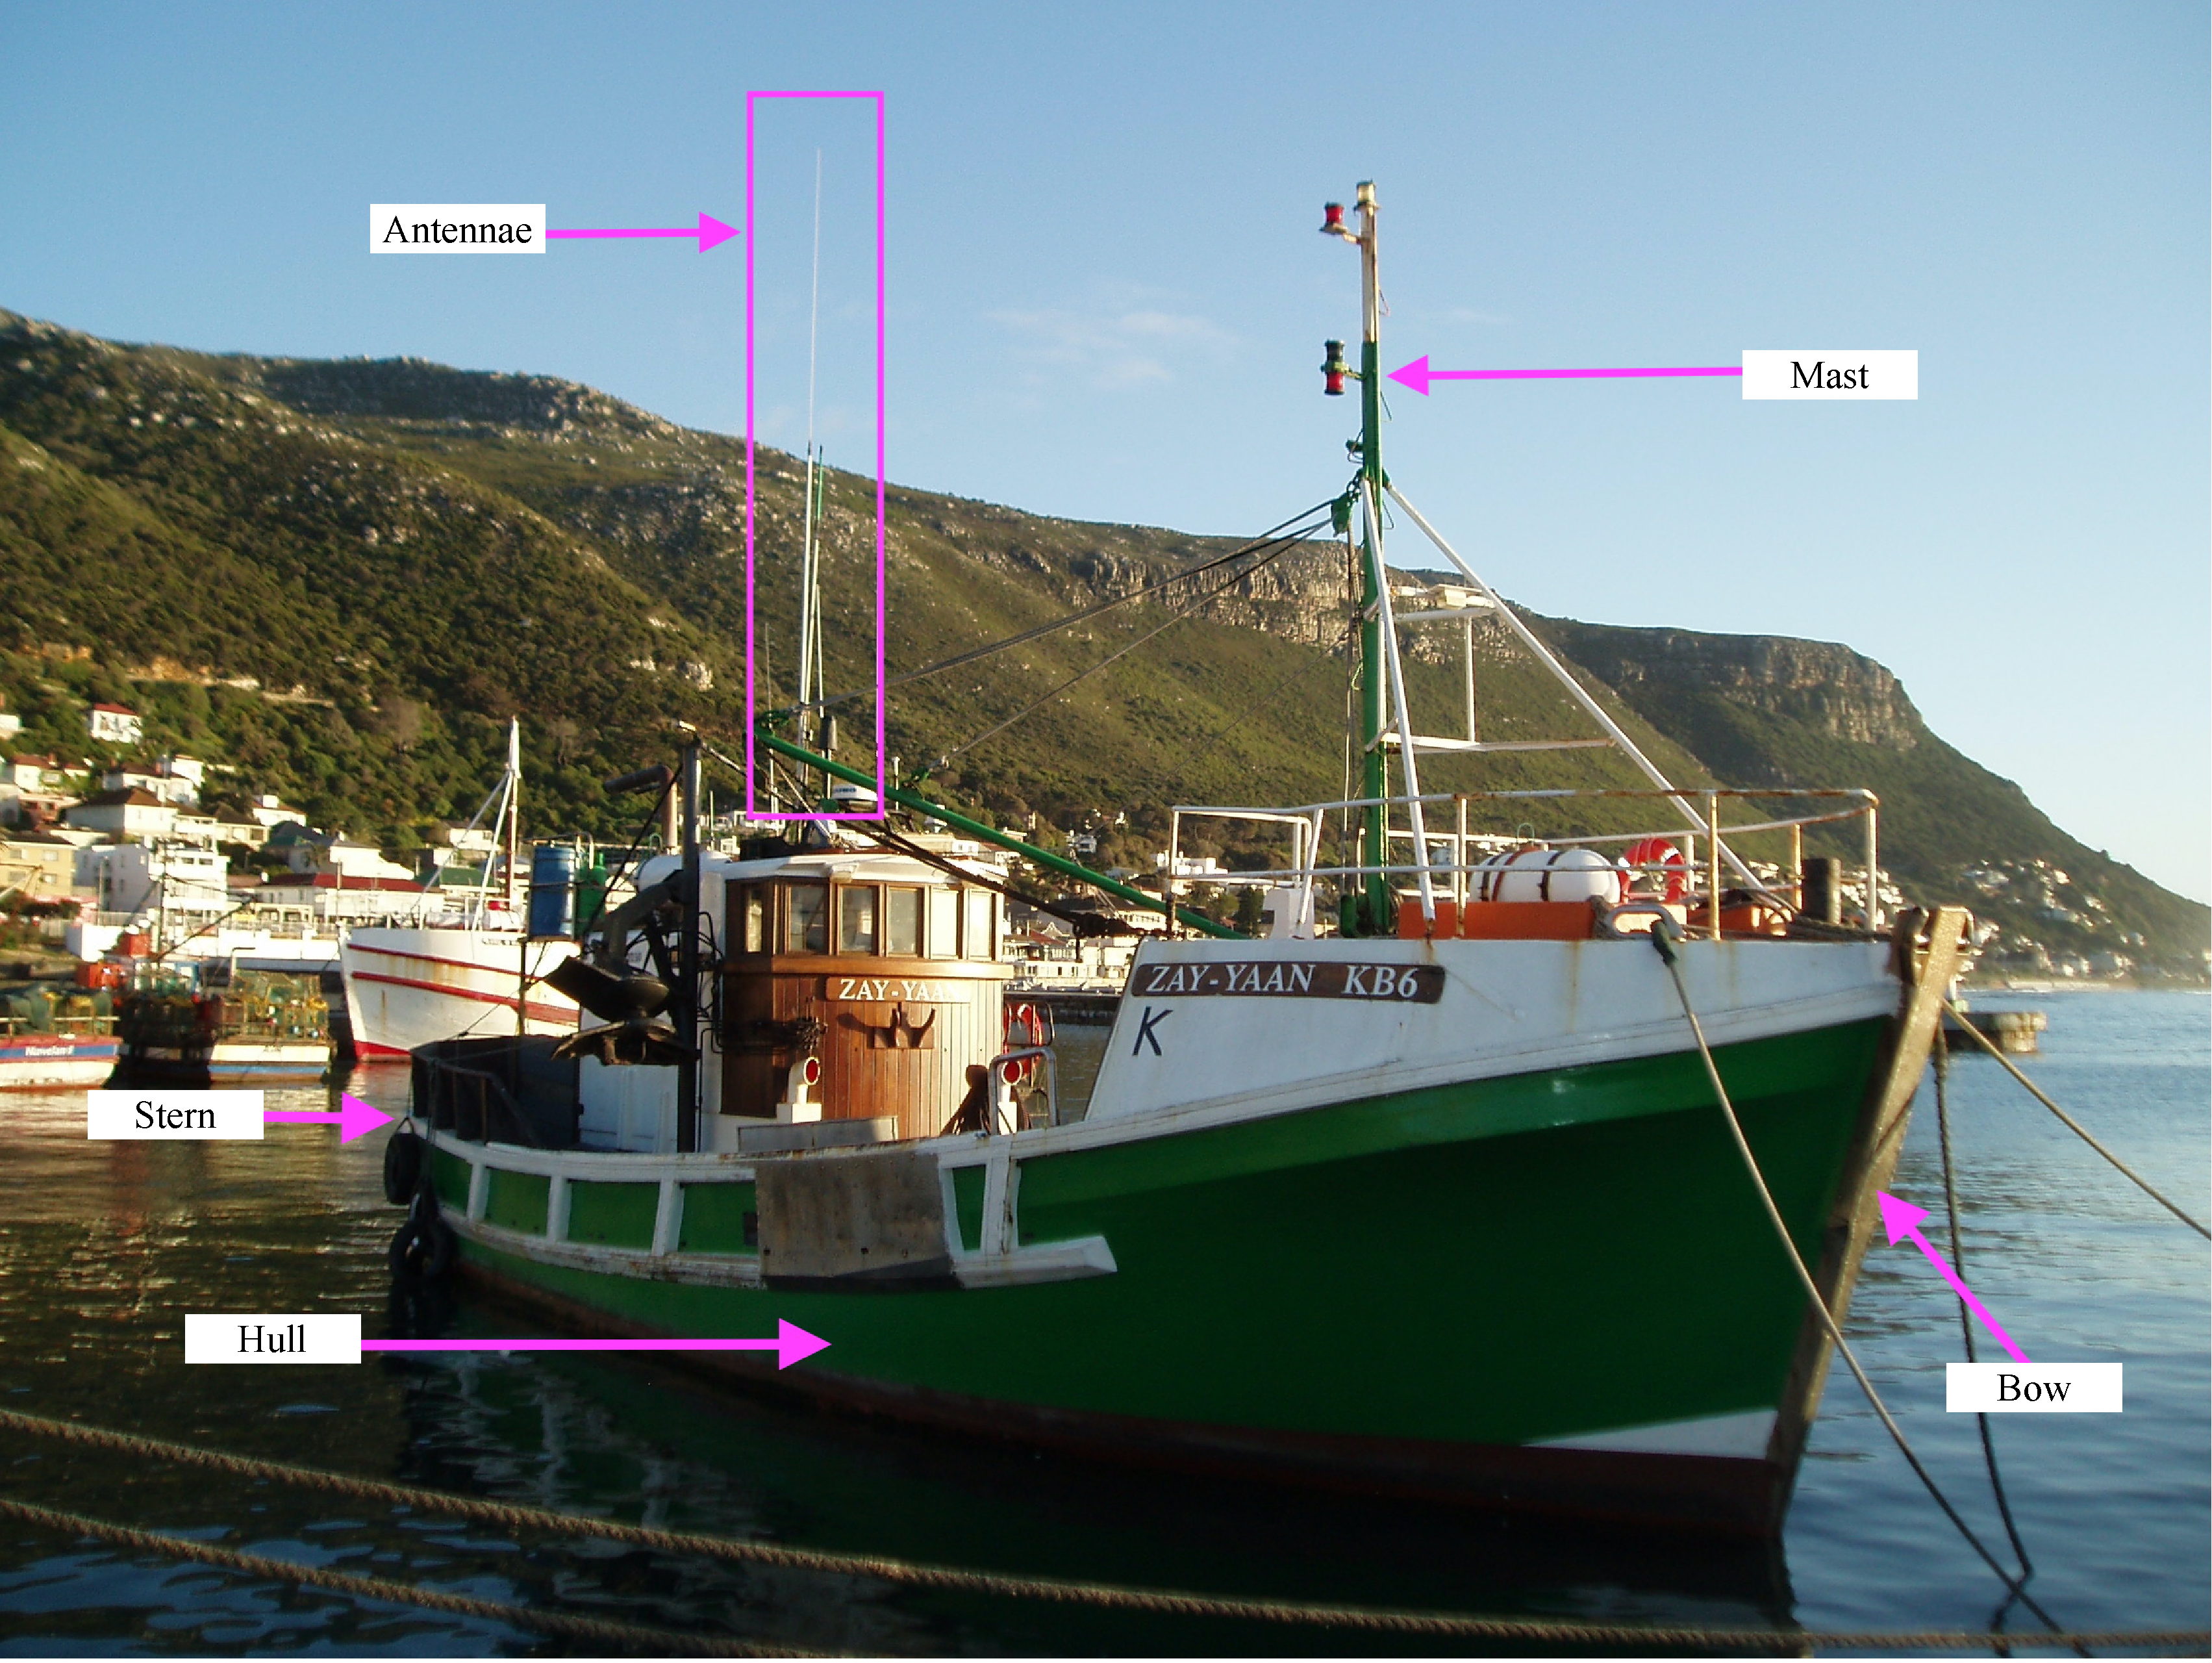
\includegraphics{Figures/04AlgoV&V/Measured/zayyaan.pdf}}
    \caption{Zay-Yaan KB6 boat structure. Adapted from \cite{zayyaan_data}.}
    \label{fig:zayyaan}
\end{figure}

Several frames\footnote{A frame is a single \gls{isar} image developed using a preselcted number of \gls{hrr} profiles. In this report it was 128 profiles.} were considered for use in validation. The \gls{isar} image frames and \gls{hrr} profiles in \autoref{fig:measured_data_frames} were constructed from a single measured data set. As discussed in \autoref{sec:theory_cptwl}, the size of the \gls{cptwl} affects the quality of the image. In this report, the \gls{cptwl} was fixed at 128, and it served as the constant value for all the frames. The frames considered in this section were chosen from the larger subset as they all produce \gls{isar} images that resemble the side-view of the boat. 

    \begin{figure}[H]
        \begin{minipage}{0.9\linewidth}
            \begin{figure}
                \begin{tabular}{@{}cccc@{}}
                    \begin{subfigure}{0.25\linewidth}
                        \centering
                        \resizebox{\linewidth}{!}{% This file was created by matlab2tikz.
%
%The latest updates can be retrieved from
%  http://www.mathworks.com/matlabcentral/fileexchange/22022-matlab2tikz-matlab2tikz
%where you can also make suggestions and rate matlab2tikz.
%
\begin{tikzpicture}

\begin{axis}[%
width=5.554in,
height=4.754in,
at={(0.932in,0.642in)},
scale only axis,
    point meta min=-3.40262853181023,
point meta max=70.6498190084972,
axis on top,
xmin=-0.15609375,
xmax=29.81390625,
xlabel style={font=\color{white!15!black}},
xlabel={Range (m)},
y dir=reverse,
ymin=0.5,
ymax=128.5,
ylabel style={font=\color{white!15!black}},
ylabel={Profile Number},
axis background/.style={fill=white},
colormap/jet,
colorbar
]
\addplot [forget plot] graphics [xmin=-0.15609375, xmax=29.81390625, ymin=0.5, ymax=128.5] {Figures/09Appendix/MeasuredDataFrames/Measured_HRRP_2464.png};
\end{axis}
\end{tikzpicture}%}
                        \caption{Frame 1: unaligned HRR profiles. \label{subfig:measured_data_frames_HRRP_frame1}}
                    \end{subfigure}
                    &
                    \begin{subfigure}{0.25\linewidth}
                        \centering
                        \resizebox{\linewidth}{!}{% This file was created by matlab2tikz.
%
%The latest updates can be retrieved from
%  http://www.mathworks.com/matlabcentral/fileexchange/22022-matlab2tikz-matlab2tikz
%where you can also make suggestions and rate matlab2tikz.
%
\begin{tikzpicture}

\begin{axis}[%
width=5.554in,
height=4.754in,
at={(0.932in,0.642in)},
scale only axis,
    point meta min=-3.40262853181023,
point meta max=70.6498190084972,
axis on top,
xmin=-0.15609375,
xmax=29.81390625,
xlabel style={font=\color{white!15!black}},
xlabel={Range (m)},
y dir=reverse,
ymin=0.5,
ymax=128.5,
ylabel style={font=\color{white!15!black}},
ylabel={Profile Number},
axis background/.style={fill=white},
colormap/jet,
colorbar
]
\addplot [forget plot] graphics [xmin=-0.15609375, xmax=29.81390625, ymin=0.5, ymax=128.5] {Figures/09Appendix/MeasuredDataFrames/Measured_HRRP_2970.png};
\end{axis}
\end{tikzpicture}%}
                        \caption{Frame 2: unaligned HRR profiles.\label{subfig:measured_data_frames_HRRP_frame2}}
                    \end{subfigure}
                    &
                    \begin{subfigure}{0.25\linewidth}
                        \centering
                        \resizebox{\linewidth}{!}{% This file was created by matlab2tikz.
%
%The latest updates can be retrieved from
%  http://www.mathworks.com/matlabcentral/fileexchange/22022-matlab2tikz-matlab2tikz
%where you can also make suggestions and rate matlab2tikz.
%
\begin{tikzpicture}

\begin{axis}[%
width=5.554in,
height=4.754in,
at={(0.932in,0.642in)},
scale only axis,
    point meta min=-3.40262853181023,
point meta max=70.6498190084972,
axis on top,
xmin=0,
xmax=128,
xlabel style={font=\color{white!15!black}},
xlabel={Range (m)},
y dir=reverse,
ymin=0,
ymax=96,
ylabel style={font=\color{white!15!black}},
ylabel={Profile Number},
axis background/.style={fill=white},
colormap/jet,
colorbar
]
\addplot [forget plot] graphics [xmin=0, xmax=128, ymin=0, ymax=96] {Figures/09Appendix/MeasuredDataFrames/Measured_HRRP_3827.png};
\end{axis}
\end{tikzpicture}%
}
                        \caption{Frame 3: unaligned HRR profiles.\label{subfig:measured_data_frames_HRRP_frame3}}
                    \end{subfigure}
                    &
                    \begin{subfigure}{0.25\linewidth}
                        \centering
                        \resizebox{\linewidth}{!}{
% This file was created by matlab2tikz.
%
%The latest updates can be retrieved from
%  http://www.mathworks.com/matlabcentral/fileexchange/22022-matlab2tikz-matlab2tikz
%where you can also make suggestions and rate matlab2tikz.
%
\begin{tikzpicture}

\begin{axis}[%
width=5.554in,
height=4.754in,
at={(0.932in,0.642in)},
scale only axis,
    point meta min=-3.40262853181023,
point meta max=70.6498190084972,
axis on top,
xmin=0,
xmax=128,
xlabel style={font=\color{white!15!black}},
xlabel={Range (m)},
y dir=reverse,
ymin=0,
ymax=96,
ylabel style={font=\color{white!15!black}},
ylabel={Profile Number},
axis background/.style={fill=white},
colormap/jet,
colorbar
]
\addplot [forget plot] graphics [xmin=0, xmax=128, ymin=0, ymax=96] {Figures/09Appendix/MeasuredDataFrames/Measured_HRRP_4189.png};
\end{axis}
\end{tikzpicture}%
}
                        \caption{Frame 4: unaligned HRR profiles. \label{subfig:measured_data_frames_HRRP_frame4}}
                    \end{subfigure}
                    \\
                    \begin{subfigure}{0.25\linewidth}
                        \centering
                        \resizebox{\linewidth}{!}{% This file was created by matlab2tikz.
%
%The latest updates can be retrieved from
%  http://www.mathworks.com/matlabcentral/fileexchange/22022-matlab2tikz-matlab2tikz
%where you can also make suggestions and rate matlab2tikz.
%
\begin{tikzpicture}
\begin{axis}[%
width=5.554in,
height=4.754in,
at={(0.932in,0.642in)},
scale only axis,
point meta min=-35,
point meta max=0,
axis on top,
xmin=-0.15609375,
xmax=29.81390625,
xlabel style={font=\color{white!15!black}},
xlabel={Range (m)},
ymin=-88.690863104058,
ymax=87.3049831146128,
ylabel style={font=\color{white!15!black}},
ylabel={Doppler frequency (Hz)},
axis background/.style={fill=white},
colormap/jet,
colorbar
]
\addplot [forget plot] graphics [xmin=-0.15609375, xmax=29.81390625, ymin=-88.690863104058, ymax=87.3049831146128] {Figures/09Appendix/MeasuredDataFrames/Measured_ISAR_2464.png};
\end{axis}

\end{tikzpicture}%}
                        \caption{Frame 1: unfocused ISAR image.\label{subfig:measured_data_frames_ISAR_frame1}}
                    \end{subfigure}
                    &
                    \begin{subfigure}{0.25\linewidth}
                        \centering
                        \resizebox{\linewidth}{!}{% This file was created by matlab2tikz.
%
%The latest updates can be retrieved from
%  http://www.mathworks.com/matlabcentral/fileexchange/22022-matlab2tikz-matlab2tikz
%where you can also make suggestions and rate matlab2tikz.
%
\begin{tikzpicture}
\begin{axis}[%
width=5.554in,
height=4.754in,
at={(0.932in,0.642in)},
scale only axis,
point meta min=-35,
point meta max=0,
axis on top,
xmin=-0.15609375,
xmax=29.81390625,
xlabel style={font=\color{white!15!black}},
xlabel={Range (m)},
ymin=-88.690863104058,
ymax=87.3049831146128,
ylabel style={font=\color{white!15!black}},
ylabel={Doppler frequency (Hz)},
axis background/.style={fill=white},
colormap/jet,
colorbar
]
\addplot [forget plot] graphics [xmin=-0.15609375, xmax=29.81390625, ymin=-88.690863104058, ymax=87.3049831146128] {Figures/09Appendix/MeasuredDataFrames/Measured_ISAR_2970.png};
\end{axis}

\end{tikzpicture}%}
                        \caption{Frame 2: unfocused ISAR image.\label{subfig:measured_data_frames_ISAR_frame2}}
                    \end{subfigure}
                    &
                    \begin{subfigure}{0.25\linewidth}
                        \centering
                        \resizebox{\linewidth}{!}{% This file was created by matlab2tikz.
%
%The latest updates can be retrieved from
%  http://www.mathworks.com/matlabcentral/fileexchange/22022-matlab2tikz-matlab2tikz
%where you can also make suggestions and rate matlab2tikz.
%
\begin{tikzpicture}
\begin{axis}[%
width=5.554in,
height=4.754in,
at={(0.932in,0.642in)},
scale only axis,
point meta min=-35,
point meta max=0,
axis on top,
xmin=-0.15609375,
xmax=29.81390625,
xlabel style={font=\color{white!15!black}},
xlabel={Range (m)},
ymin=-88.690863104058,
ymax=87.3049831146128,
ylabel style={font=\color{white!15!black}},
ylabel={Doppler frequency (Hz)},
axis background/.style={fill=white},
colormap/jet,
colorbar
]
\addplot [forget plot] graphics [xmin=-0.15609375, xmax=29.81390625, ymin=-88.690863104058, ymax=87.3049831146128] {Figures/09Appendix/MeasuredDataFrames/Measured_ISAR_3827.png};
\end{axis}

\end{tikzpicture}%}
                         \caption{Frame 3: unfocused ISAR image.\label{subfig:measured_data_frames_ISAR_frame3}}
                    \end{subfigure}
                    &
                    \begin{subfigure}{0.25\linewidth}
                        \centering
                        \resizebox{\linewidth}{!}{% This file was created by matlab2tikz.
%
%The latest updates can be retrieved from
%  http://www.mathworks.com/matlabcentral/fileexchange/22022-matlab2tikz-matlab2tikz
%where you can also make suggestions and rate matlab2tikz.
%
\begin{tikzpicture}
\begin{axis}[%
width=5.554in,
height=4.754in,
at={(0.932in,0.642in)},
scale only axis,
point meta min=-35,
point meta max=0,
axis on top,
xmin=-0.15609375,
xmax=29.81390625,
xlabel style={font=\color{white!15!black}},
xlabel={Range (m)},
ymin=-88.690863104058,
ymax=87.3049831146128,
ylabel style={font=\color{white!15!black}},
ylabel={Doppler frequency (Hz)},
axis background/.style={fill=white},
colormap/jet,
colorbar
]
\addplot [forget plot] graphics [xmin=-0.15609375, xmax=29.81390625, ymin=-88.690863104058, ymax=87.3049831146128] {Figures/09Appendix/MeasuredDataFrames/Measured_ISAR_4189.png};
\end{axis}

\end{tikzpicture}%}
                         \caption{Frame 4: unfocused ISAR image.\label{subfig:measured_data_frames_ISAR_frame4}}
                    \end{subfigure}
                \end{tabular}
                \caption{Different \gls{isar} image frames produced from a single measured data set. \label{fig:measured_data_frames}}
            \end{figure}
        \end{minipage}
    \end{figure}

    Multiple frames were unsuitable for validating the \gls{ra} and \gls{af} algorithms discussed in this report due to specific characteristics. \autoref{subfig:measured_data_frames_ISAR_frame2} was not suitable because not all of the profiles appeared within the frame, which could have led to erroneous \gls{ra}. Using this frame would have created uncertainty regarding whether any unexpected results were due to poor-quality data or the implemented algorithm, making it an unsuitable choice. Additionally, \autoref{subfig:measured_data_frames_HRRP_frame3} was significantly affected by noise and had fewer prominent scatterers compared to Frames 1 and 2. This made it an unsuitable choice compared to the other frames.

    Furthermore, the profiles in \autoref{subfig:measured_data_frames_HRRP_frame1} and \autoref{subfig:measured_data_frames_HRRP_frame4} exhibited more than one clear \gls{ds} and were fully within the frame, making them suitable choices for verifying \gls{ra} algorithms. \autoref{fig:measured_data_frames_RA} shows the \gls{hrr} profiles of these two frames after applying the Correlation \gls{ra} algorithm.
    
    \begin{figure}[H]
        \centering
        \begin{subfigure}{0.4\textwidth}
            \centering
            \resizebox{\linewidth}{!}{% This file was created by matlab2tikz.
%
%The latest updates can be retrieved from
%  http://www.mathworks.com/matlabcentral/fileexchange/22022-matlab2tikz-matlab2tikz
%where you can also make suggestions and rate matlab2tikz.
%
\begin{tikzpicture}

\begin{axis}[%
width=5.554in,
height=4.754in,
at={(0.932in,0.642in)},
scale only axis,
    point meta min=-3.40262853181023,
point meta max=70.6498190084972,
axis on top,
xmin=0,
xmax=128,
xlabel style={font=\color{white!15!black}},
xlabel={Range (m)},
y dir=reverse,
ymin=0,
ymax=96,
ylabel style={font=\color{white!15!black}},
ylabel={Profile Number},
axis background/.style={fill=white},
colormap/jet,
colorbar
]
\addplot [forget plot] graphics [xmin=0, xmax=128, ymin=0, ymax=96] {Figures/09Appendix/MeasuredDataFrames/Measured_SCRA_HRRP_2464.png};

% Labels
\draw[->, black, line width=1.5pt] (35, 50) -- (57.75, 10);
\draw[->, black, line width=1.5pt] (35, 50) -- (56.5, 50);
\draw[->, black, line width=1.5pt] (35, 50) -- (57.75, 88);
\node[left] at (36, 50) {\tikz[baseline] \node[fill=white,inner sep=2pt] {Scatterer A};};

% Labels
\node[left] at (36, 50) {\tikz[baseline] \node[fill=white,inner sep=2pt] {Scatterer A};};
\draw[black, line width=1.5pt] (58 - 1, 96) rectangle (58 + 1, 0);

\end{axis}
\end{tikzpicture}%}
        \end{subfigure}
        \begin{subfigure}{0.4\textwidth}
            \centering
            \resizebox{\linewidth}{!}{% This file was created by matlab2tikz.
%
%The latest updates can be retrieved from
%  http://www.mathworks.com/matlabcentral/fileexchange/22022-matlab2tikz-matlab2tikz
%where you can also make suggestions and rate matlab2tikz.
%
\begin{tikzpicture}

\begin{axis}[%
width=5.554in,
height=4.754in,
at={(0.932in,0.642in)},
scale only axis,
    point meta min=-3.40262853181023,
point meta max=70.6498190084972,
axis on top,
xmin=0,
xmax=128,
xlabel style={font=\color{white!15!black}},
xlabel={Range (m)},
y dir=reverse,
ymin=0,
ymax=96,
ylabel style={font=\color{white!15!black}},
ylabel={Profile Number},
axis background/.style={fill=white},
colormap/jet,
colorbar
]
\addplot [forget plot] graphics [xmin=0, xmax=128, ymin=0, ymax=96] {Figures/09Appendix/MeasuredDataFrames/Measured_SCRA_HRRP_4189.png};

% Labels
\draw[->, black, line width=1.5pt] (35, 50) -- (60, 50);
\node[left] at (36, 50) {\tikz[baseline] \node[fill=white,inner sep=2pt] {Scatterer A};};
\draw[black, line width=1.5pt] (61.5 - 1, 96) rectangle (61.5 + 1, 0);

\end{axis}
\end{tikzpicture}%} 
        \end{subfigure}
        \caption{Frame 1 (left) and 4 (right): range-aligned \gls{hrr} profiles.} \label{fig:measured_data_frames_RA}
    \end{figure}

    As discussed in \autoref{subsec:theory_isar}, not all frames of \gls{isar} data can be focused due to factors such as the object's motion and the \gls{cptwl}. Consequently, it was expected that some measured data frames would not be perfectly range-aligned or autofocused. For the purpose of validation testing, it was essential to select ideal data that gave the \gls{tmc} algorithms the best chance at success, since the aim was to demonstrate the performance of the algorithms on measured data.

    When comparing the profile frames in \autoref{fig:measured_data_frames_RA}, it was clear that the profiles in Frame 1 were better aligned than those in Frame 4. Moreover, Frame 1 featured a prominent Scatterer A that was consistently visible at range bin 57 across all range profiles, making it an ideal choice for \gls{af} validation. In contrast, Scatterer A in Frame 4 did not exhibit the same level of consistent visibility in all profiles. Using Frame 4 for validation testing would have introduced uncertainty surrounding whether any unexpected results in \gls{af} were caused by poor-quality data or the implemented algorithm. For these reasons, \textbf{Frame 1 in \autoref{fig:measured_data_frames_RA}  was selected} for validation testing in this chapter.

    A \textsc{MATLAB} script was used to facilitate the validation testing process. Permission was obtained from the \gls{csir} to use their measured data but is not freely available for replicating the measured data results in this report. 
%%%%%%%%%%%%%%%%%%%%%%%%%%%%%%%%%%%%%%%%%%%%%%%%%%%%%%%%%%%%%%%%%%%%%%%%%%%%%%%%%%%%%%%%%%%%%%%%%%%%
\section{Correlation Range Alignment Algorithm}\label{subsec:corrRA}
This is a simplistic \gls{ra} algorithm that uses cross-correlation to determine the number of integer range bins by which a profile is misaligned with respect to a reference profile. The calculated number of bins is used to shift the misaligned range profile into alignment with the reference profile. An outline of the correlation \gls{ra} algorithm as described in Chapter 4.1.1. \cite{ISARtextbook_Martorella} is given in \autoref{alg:corr_RA}.
    %***************************************************************************************%
    \subsection{Pseudo Code and Implementation}
    % Corr RA Pseudo code
    \begin{figure}[H]
      \vspace{0.5cm}
      \centering
      \captionsetup{type=figure}
      \begin{minipage}{.7\linewidth}
        \begin{algorithm}[H]
            \caption{Correlation \gls{ra} Algorithm.\label{alg:corr_RA}}
            
            \LinesNumbered % NUMBER THE LINES
            \DontPrintSemicolon
            \SetAlgoLined
            \SetKwInOut{Input}{input}\SetKwInOut{Output}{output}\SetKwInOut{Parameter}{parameter}
    
            \Input{All \gls{hrrp}s, matrix $hrrp_{all}$}
            \Output{Range-aligned \gls{hrrp}s, matrix $hrrp_{RA}$}
            \Parameter{Reference \gls{hrrp} number, $refIndex$}
            
            \BlankLine
            \Begin{
                $hrrp_{ref}\leftarrow hrrp_{all}[refIndex] $\;
                $correlation  \leftarrow $ auto-cross-correlate $hrrp_{ref}$\;
                $peakIndex_{ref} \leftarrow$ index of $max(correlation)$\;
                \For(){k in 1 to rows($hrrp_{all}$)}{
                    $correlation  \leftarrow $ cross-correlate $hrrp_{all}[k]$ and $hrrp_{ref}$ \;
                    $peakIndex \leftarrow$ index of $max(correlation)$\;
                    $shift \leftarrow peakIndex_{ref} - peakIndex $\;
                    $hrrp_{RA}[k] \leftarrow circularshift$ $hrrp_{all}[k]$ by $shift$\; 
                }
            }
          \vspace{0.5cm}
        \end{algorithm}
      \end{minipage}
    \end{figure}

    The Correlation Algorithm, \autoref{alg:corr_RA}, was implemented as a stand-alone function in \textsc{MATLAB}. The function, \href{}{corrRA.m}, was validated and verified in this section.
    
    %***************************************************************************************%
    \subsection{Algorithm Verification}
    In this subsection simulated \gls{hrr} profiles were used to verify that \autoref{alg:corr_RA} was implemented correctly in \textsc{MATLAB}. 
    
    % Grid of the HRRP 
    \begin{figure}[H]
        \begin{minipage}{0.60\linewidth}
            \begin{figure}
                \begin{tabular}{@{}cc@{}}
                    \begin{subfigure}{0.5\linewidth}
                        \centering
                        \resizebox{\linewidth}{!}{% This file was created by matlab2tikz.
%
%The latest updates can be retrieved from
%  http://www.mathworks.com/matlabcentral/fileexchange/22022-matlab2tikz-matlab2tikz
%where you can also make suggestions and rate matlab2tikz.
%
\begin{tikzpicture}
\begin{axis}[%
width=5.554in,
height=4.754in,
at={(0.932in,0.642in)},
scale only axis,
point meta min=-35,
point meta max=0,
axis on top,
xmin=0,
xmax=256,
xlabel style={font=\fontsize{25}{14}\selectfont\color{black}, yshift=-10pt},
xlabel={Range (m)},
y dir=reverse,
ymin=0.5,
ymax=32.5,
ylabel style={font=\fontsize{25}{14}\selectfont\color{black}, yshift=10pt},
ylabel={Profile Number},
axis background/.style={fill=white},
tick label style={font=\fontsize{20}{11}\selectfont\color{black}},
xtick distance= 50,             % Set the spacing between x-axis ticks
colormap/jet,
colorbar
]
\addplot [forget plot] graphics [xmin=0, xmax=256, ymin=0.5, ymax=32.5] {Figures/04AlgoV&V/Simulation/01WithMotion/Sim_HRRP_1mps_6deg.png};

% Add a vertical black line at x = 50
\addplot [black, line width=2pt] coordinates {(56, 0.5) (56, 32.5)};

% Add a black arrow pointing at (60, 30)
\draw[->, black, line width=1.5pt] (45, 31) -- (61, 31);
\draw[->, black, line width=1.5pt] (45, 20) -- (60, 20);
\draw[->, black, line width=1.5pt] (45, 11) -- (59, 11);
% Add a label to the left of the arrow with a white box
\node[left] at (50, 31) {\tikz[baseline] \node[fill=white,inner sep=2pt] {Scatterer A};};
\node[left] at (51, 20) {\tikz[baseline] \node[fill=white,inner sep=2pt] {Scatterer A};};
\node[left] at (52, 11) {\tikz[baseline] \node[fill=white,inner sep=2pt] {Scatterer A};};


\end{axis}
\end{tikzpicture}%
}
                        \caption{Unaligned profiles.}\label{subfig:corrRA_sim_hrrp_1mps}
                    \end{subfigure}
                    &
                    \begin{subfigure}{0.5\linewidth}
                        \centering
                        \resizebox{\linewidth}{!}{% This file was created by matlab2tikz.
%
%The latest updates can be retrieved from
%  http://www.mathworks.com/matlabcentral/fileexchange/22022-matlab2tikz-matlab2tikz
%where you can also make suggestions and rate matlab2tikz.
%
\begin{tikzpicture}
\begin{axis}[%
width=5.554in,
height=4.754in,
at={(0.932in,0.642in)},
scale only axis,
point meta min=-35,
point meta max=0,
axis on top,
xmin=-0.0732421875,
xmax=37.4267578125,
xlabel style={font=\fontsize{25}{14}\selectfont\color{black}, yshift=-10pt},
xlabel={Range (m)},
y dir=reverse,
ymin=0.5,
ymax=32.5,
ylabel style={font=\fontsize{25}{14}\selectfont\color{black}, yshift=10pt},
ylabel={Profile Number},
axis background/.style={fill=white},
tick label style={font=\fontsize{20}{11}\selectfont\color{black}},
xtick distance= 4,             % Set the spacing between x-axis ticks
colormap/jet,
colorbar
]
\addplot [forget plot] graphics [xmin=-0.0732421875, xmax=37.4267578125, ymin=0.5, ymax=32.5] {Figures/04AlgoV&V/02CorrRA/SCRA_Sim_HRRP_1mps_6deg.png};
\end{axis}
\end{tikzpicture}%}
                        \caption{Range-aligned profiles.}\label{subfig:corrRA_sim_hrrp}
                    \end{subfigure}
                \end{tabular}
                \caption{Simulated \gls{hrr} profiles before and after Correlation \gls{ra}. \label{fig:corrRA_sim}}
            \end{figure}
        \end{minipage}
        \hfill
        \begin{minipage}{0.30\linewidth}
            \begin{figure}
                \begin{tabular}{@{}c@{}}
                    \begin{subfigure}{\linewidth}
                        \centering
                        \resizebox{\linewidth}{!}{% This file was created by matlab2tikz.
%
%The latest updates can be retrieved from
%  http://www.mathworks.com/matlabcentral/fileexchange/22022-matlab2tikz-matlab2tikz
%where you can also make suggestions and rate matlab2tikz.
%
\begin{tikzpicture}
\begin{axis}[%
width=5.554in,
height=4.754in,
at={(0.932in,0.642in)},
scale only axis,
point meta min=-35,
point meta max=0,
axis on top,
xmin=0,
xmax=256,
xlabel style={font=\fontsize{25}{14}\selectfont\color{black}, yshift=-10pt},
xlabel={Range (m)},
y dir=reverse,
ymin=0.5,
ymax=32.5,
ylabel style={font=\fontsize{25}{14}\selectfont\color{black}, yshift=10pt},
ylabel={Profile Number},
axis background/.style={fill=white},
tick label style={font=\fontsize{20}{11}\selectfont\color{black}},
xtick distance= 50,             % Set the spacing between x-axis ticks
colormap/jet,
colorbar
]
\addplot [forget plot] graphics [xmin=0, xmax=256, ymin=0.5, ymax=32.5] {Figures/04AlgoV&V/Simulation/00NoMotion/Sim_HRRP_0mps_6deg.png};
\end{axis}
\end{tikzpicture}%}
                        \caption{Focused profiles.\label{subfig:corrRA_sim_hrrp_0mps}}
                    \end{subfigure}
                \end{tabular}
                \caption{Simulated object with no translation motion.} \label{fig:sim_0mps}
            \end{figure}
        \end{minipage}
    \end{figure}
    
    Recall from \autoref{theory:RA} that an object's motion causes range migration of the object between range profiles. \autoref{subfig:corrRA_sim_hrrp_1mps} shows that Scatterer A migrated between profiles as expected, the vertical line further illustrates that the profiles were not aligned. Correlation \gls{ra} was applied to the unaligned profiles in an attempt to achieve straight line scatterers similar to profiles of the object without translation motion shown in \autoref{subfig:corrRA_sim_hrrp_0mps}.

    Using line 7 of \autoref{alg:corr_RA}, the peak location (index) of each profile's cross-correlation with respect to profile 1 was calculated. This value was then used to calculate the number of bins each profile was shifted from profile 1 as in line 8 of \autoref{alg:corr_RA}. \autoref{fig:corrRA_sim_shifts} shows the calculated bin shifts for each profile in \autoref{fig:corrRA_sim_shifts}.

    \begin{figure}[H]
        \centering
        \resizebox{0.4\linewidth}{!}{% This file was created by matlab2tikz.
%
%The latest updates can be retrieved from
%  http://www.mathworks.com/matlabcentral/fileexchange/22022-matlab2tikz-matlab2tikz
%where you can also make suggestions and rate matlab2tikz.
%
\definecolor{mycolor1}{rgb}{0.00000,0.44700,0.74100}%
%
\begin{tikzpicture}

\begin{axis}[%
width=6.028in,
height=4.754in,
at={(1.011in,0.642in)},
scale only axis,
xmin=0,
xmax=35,
xlabel style={font=\fontsize{20}{20}\selectfont\color{black}, yshift = -10},
xlabel={Profile Number},
ymin=-4,
ymax=0,
ylabel style={font=\fontsize{20}{20}\selectfont\color{black}},
ylabel={Number of bin shifts},
axis background/.style={fill=white},
tick label style={font=\fontsize{15}{11}\selectfont\color{black}},
xtick distance= 4            % Set the spacing between x-axis ticks
]
\addplot [color=mycolor1, forget plot]
  table[row sep=crcr]
        \caption{Staircase curve of range bin shifts per \gls{hrrp} for Correlation \gls{ra} on simulated profiles.\label{fig:corrRA_sim_shifts}}
    \end{figure}

    \autoref{subfig:corrRA_sim_hrrp_1mps} shows that Scatterer A migrated by a fraction of a range bin between successive profiles. However, the 'steps' in \autoref{fig:corrRA_sim_shifts} show that each profile was always shifted by an integer number of bins. As explained before, the bin shifts were calculated as the difference between array indices which was an integer value. Therefore, profiles with fractional bin shifts were rather treated as a full bin shift as shown by the flat horizontal steps in \autoref{fig:corrRA_sim_shifts}. In terms of the algorithm, which expects all bin shifts to be integer numbers, \autoref{fig:corrRA_sim_shifts} was correct.

    Applying the implemented \autoref{alg:corr_RA} to the unaligned profiles in \autoref{subfig:corrRA_sim_hrrp_1mps} did not produce range-aligned profiles in \autoref{subfig:corrRA_sim_hrrp} that look like the profiles in \autoref{subfig:corrRA_sim_hrrp_0mps}. However, the range-aligned profiles do follow the staircase pattern of \autoref{fig:corrRA_sim_shifts}. Although, the profiles were not perfectly aligned as expected, they were correctly aligned in terms of the bin shift values in \autoref{alg:corr_RA}. Therefore, because the correct bin shifts were calculated and applied, \autoref{alg:corr_RA} was implemented correctly.

    %***************************************************************************************%
    \subsection{Algorithm Validation}
    In this subsection, measured \gls{hrr} data was used to validate that the implemented Correlation \gls{ra} did range-align the \gls{hrr} profiles.
    
    % Grid of the HRRP 
    \begin{figure}[H]
        \centering
        \begin{subfigure}{0.4\linewidth}
                \centering
                \resizebox{\linewidth}{!}{% This file was created by matlab2tikz.
%
%The latest updates can be retrieved from
%  http://www.mathworks.com/matlabcentral/fileexchange/22022-matlab2tikz-matlab2tikz
%where you can also make suggestions and rate matlab2tikz.
%
\begin{tikzpicture}
\begin{axis}[%
width=5.554in,
height=4.754in,
at={(0.932in,0.642in)},
scale only axis,
point meta min=-35,
point meta max=0,
axis on top,
xmin=0,
xmax=128,
xlabel style={font=\fontsize{25}{14}\selectfont\color{black}, yshift=-10pt},
xlabel={Range Bin Number},
y dir=reverse,
ymin=0,
ymax=96,
ylabel style={font=\fontsize{25}{14}\selectfont\color{black}, yshift=10pt},
ylabel={Profile Number},
axis background/.style={fill=white},
tick label style={font=\fontsize{20}{11}\selectfont\color{black}},
xtick distance= 20,             % Set the spacing between x-axis ticks
colormap/jet,
colorbar
]
\addplot [forget plot] graphics [xmin=0, xmax=128, ymin=0, ymax=96] {Figures/04AlgoV&V/Measured/01Original/Measured_HRRP_frame2464.png};

% Add a vertical black line at x = 50
\addplot [black, line width=2pt] coordinates {(59, 0) (59, 96)};

% Add a black arrow pointing at (60, 30)
\draw[->, black, line width=1.5pt] (35, 8) -- (57.5, 8);
\draw[->, black, line width=1.5pt] (35, 18) -- (56, 18);
\draw[->, black, line width=1.5pt] (30, 76) -- (50.5, 76);
% Add a label to the left of the arrow with a white box
\node[left] at (36, 8) {\tikz[baseline] \node[fill=white,inner sep=2pt] {Scatterer A};};
\node[left] at (36, 18) {\tikz[baseline] \node[fill=white,inner sep=2pt] {Scatterer A};};
\node[left] at (30, 76) {\tikz[baseline] \node[fill=white,inner sep=2pt] {Scatterer A};};

\end{axis}
\end{tikzpicture}%}
                \caption{Unaligned profiles.\label{subfig:corrRA_measured_hrrp_unaligned}}
        \end{subfigure}
        \hspace{1cm}
        \begin{subfigure}{0.4\linewidth}
                \centering
                \resizebox{\linewidth}{!}{% This file was created by matlab2tikz.
%
%The latest updates can be retrieved from
%  http://www.mathworks.com/matlabcentral/fileexchange/22022-matlab2tikz-matlab2tikz
%where you can also make suggestions and rate matlab2tikz.
%
\begin{tikzpicture}
\begin{axis}[%
width=5.554in,
height=4.754in,
at={(0.932in,0.642in)},
scale only axis,
point meta min=-35,
point meta max=0,
axis on top,
xmin=0,
xmax=128,
xlabel style={font=\fontsize{25}{14}\selectfont\color{black}, yshift=-10pt},
xlabel={Range Bin Number},
y dir=reverse,
ymin=0,
ymax=96,
ylabel style={font=\fontsize{25}{14}\selectfont\color{black}, yshift=10pt},
ylabel={Profile Number},
axis background/.style={fill=white},
tick label style={font=\fontsize{20}{11}\selectfont\color{black}},
xtick distance= 20,             % Set the spacing between x-axis ticks
colormap/jet,
colorbar
]
\addplot [forget plot] graphics [xmin=0, xmax=128, ymin=0, ymax=96] {Figures/04AlgoV&V/Measured/02CorrRA/SCRA_Measured_HRRP_frame2464.png};

% Add a vertical black line at x = 50
\addplot [black, line width=2pt] coordinates {(59, 0) (59, 96)};

% Add pink arrows pointing at (60, 30)
\draw[->, black, line width=1.5pt] (35, 8) -- (57.5, 8);
\draw[->,black, line width=1.5pt] (35, 18) -- (57.5, 18);
\draw[->,black, line width=1.5pt] (35, 76) -- (57.5, 76);
% Add a label to the left of the arrow with a white box
\node[left] at (36, 8) {\tikz[baseline] \node[fill=white,inner sep=2pt] {Scatterer A};};
\node[left] at (36, 18) {\tikz[baseline] \node[fill=white,inner sep=2pt] {Scatterer A};};
\node[left] at (36, 76) {\tikz[baseline] \node[fill=white,inner sep=2pt] {Scatterer A};};

\end{axis}
\end{tikzpicture}%}
                \caption{Range-aligned profiles.\label{subfig:corrRA_measureed_hrrp}}
        \end{subfigure}
        \caption{\gls{hrr} profiles of measured data frame before and after Correlation \gls{ra}. \label{fig:corrRA_measured}}
    \end{figure}

    \autoref{subfig:corrRA_measured_hrrp_unaligned} shows that Scatterer A migrated between profiles. Comparing the position of Scatterer A, in all profiles, to the vertical black line in \autoref{subfig:corrRA_measured_hrrp_unaligned} illustrates that before \gls{ra}, the profiles were not aligned to profile 1.
    
    \begin{figure}[H]
        \centering
        \resizebox{0.4\linewidth}{!}{% This file was created by matlab2tikz.
%
%The latest updates can be retrieved from
%  http://www.mathworks.com/matlabcentral/fileexchange/22022-matlab2tikz-matlab2tikz
%where you can also make suggestions and rate matlab2tikz.
%
\definecolor{mycolor1}{rgb}{0.00000,0.44700,0.74100}%
%
\begin{tikzpicture}

\begin{axis}[%
width=6.028in,
height=4.754in,
at={(1.011in,0.642in)},
scale only axis,
xmin=0,
xmax=128,
xlabel style={font=\fontsize{20}{20}\selectfont\color{black}, yshift=-10pt},
xlabel={Profile Number},
ymin=0,
ymax=7,
ylabel style={font=\fontsize{20}{20}\selectfont\color{black}, yshift=10pt},
ylabel={Number of bin shifts},
axis background/.style={fill=white},
xtick distance = 20,
tick label style={font=\fontsize{15}{11}\selectfont\color{black}},
ytick={0,1,2,3,4,5,6,7}, % Set the y-axis ticks explicitly
grid = both
]
\addplot [color=mycolor1,forget plot]
  table[row sep=crcr]{%
1	0\\
2	0\\
3	0\\
4	0\\
5	0\\
6	0\\
7	0\\
8	0\\
9	0\\
10	0\\
11	0\\
12	0\\
13	1\\
14	0\\
15	1\\
16	1\\
17	1\\
18	1\\
19	1\\
20	1\\
21	1\\
22	1\\
23	1\\
24	1\\
25	1\\
26	1\\
27	1\\
28	1\\
29	1\\
30	1\\
31	1\\
32	1\\
33	1\\
34	1\\
35	1\\
36	2\\
37	2\\
38	2\\
39	2\\
40	2\\
41	2\\
42	2\\
43	2\\
44	2\\
45	2\\
46	2\\
47	2\\
48	2\\
49	2\\
50	2\\
51	2\\
52	2\\
53	2\\
54	3\\
55	3\\
56	3\\
57	2\\
58	3\\
59	3\\
60	3\\
61	3\\
62	3\\
63	3\\
64	3\\
65	3\\
66	3\\
67	3\\
68	3\\
69	3\\
70	3\\
71	3\\
72	3\\
73	3\\
74	3\\
75	3\\
76	3\\
77	4\\
78	4\\
79	4\\
80	4\\
81	4\\
82	4\\
83	4\\
84	4\\
85	4\\
86	4\\
87	5\\
88	4\\
89	4\\
90	5\\
91	5\\
92	5\\
93	5\\
94	5\\
95	5\\
96	5\\
97	5\\
98	5\\
99	5\\
100	5\\
101	5\\
102	5\\
103	5\\
104	5\\
105	5\\
106	5\\
107	5\\
108	5\\
109	5\\
110	5\\
111	5\\
112	5\\
113	5\\
114	5\\
115	6\\
116	6\\
117	6\\
118	6\\
119	6\\
120	6\\
121	6\\
122	6\\
123	6\\
124	6\\
125	6\\
126	6\\
127	6\\
128	6\\
};
\end{axis}
\end{tikzpicture}%}
        \caption{Staircase curve of range bin shifts per \gls{hrrp} for Correlation \gls{ra} on measured profiles.}\label{fig:corrRA_Measured_shifts}
    \end{figure}
    
    \autoref{fig:corrRA_Measured_shifts} shows the bin shifts for all profiles, calculated with respect to profile 1, in \autoref{subfig:corrRA_measured_hrrp_unaligned}. These shifts were applied to the unaligned profiles and resulted in the range-aligned profiles in \autoref{subfig:corrRA_measured_hrrp}. \autoref{subfig:corrRA_measured_hrrp} shows that after range-alignment, Scatterer A remained in the same range bin throughout all profiles. Additionally, all scatterers were aligned with the vertical black line. Therefore, performing Correlation \gls{ra} range-aligned the profiles and was validated for use in this report.
    
%%%%%%%%%%%%%%%%%%%%%%%%%%%%%%%%%%%%%%%%%%%%%%%%%%%%%%%%%%%%%%%%%%%%%%%%%%%%%%%%%%%%%%%%%%%%%%%%%%%%%%%%%%%%%%%%%%%%%%%%%%%%%%%%%%%%%%%%%%%%%%%%%%%%%%%%%%%%%%%%%%%%%%%%%%%%%%%%
\section{Haywood's Range Alignment Algorithm}\label{subsec:HayRA}
This \gls{ra} algorithm realised fractional bin shifts, unlike the integer-only range bin shifts allowed in \autoref{alg:corr_RA}. This is achieved by linearising the calculated bin shifts and applying them to the profiles as a phase shift, $\phi$. The Haywood \gls{ra} algorithm, as described in \cite{haywood_RA_AF,zyweck}, was outlined in \autoref{alg:haywood_RA}.
    \subsection{Pseudo code and Implementation}
    % Haywood RA Pseudo code
    \begin{figure}[H]
      \vspace{0.5cm}
      \centering
      \captionsetup{type=figure}
      \begin{minipage}{.7\linewidth}
        \begin{algorithm}[H]
        \caption{Haywood \gls{ra} Algorithm.\label{alg:haywood_RA}}
    
        \LinesNumbered % NUMBER THE LINES
        \DontPrintSemicolon
        \SetAlgoLined
        \SetKwInOut{Input}{input}\SetKwInOut{Output}{output}\SetKwInOut{Parameter}{parameter}
    
        \Input{All \gls{hrrp}s, matrix $hrrp_{all}$}
        \Output{Range-aligned \gls{hrrp}s, matrix $hrrp_{RA}$}
        \Parameter{Reference \gls{hrrp} number, $refIndex$}
    
        \BlankLine
        \Begin{
            $hrrp_{ref}\leftarrow hrrp_{all}[refIndex] $\;
            \For(){$k$ in 1 to rows($hrrp_{all})$}{
                $correlation[k]  \leftarrow $ cross-correlate $hrrp_{all}[k]$ and $hrrp_{ref}$ \;
                $peakIndex[k] \leftarrow$ index of $\max(correlation[k] )$\;
            }
            $shifts \leftarrow$  linearise $peakIndex$\;
            $N \leftarrow$ length($shifts$)\;
            
            \For(){$k$ in 1 to rows($hrrp_{all}$)}{
                \For(){$n$ in 1 to $N$}{
                    $\phi[n] \leftarrow \exp(-j \cdot shifts[k] \cdot \frac{n}{N})$\;
                }
                $hrrp_{RA}[k] \leftarrow IFFT( \phi \cdot FFT(hrrp_{all}[k]) )$\;
            }
        }
        \vspace{0.5cm}
        \end{algorithm}
      \end{minipage}
    \end{figure}

    The \gls{ra} algorithm, \autoref{alg:haywood_RA}, was implemented as a stand-alone function in \textsc{MATLAB}. The implementation, \href{}{haywoodRA.m}, was validated and verified in this section.
    
    %***************************************************************************************%
    \subsection{Algorithm Verification}\label{subsec:corrRA_verification}
     In this subsection simulated \gls{hrr} profiles were used to verify that \autoref{alg:haywood_RA} was implemented correctly in \textsc{MATLAB}.

    The vertical black line in \autoref{subfig:hayRA_sim_hrrp} shows that the range profiles were not originally aligned. Haywood's \gls{ra} algorithm was applied to the unaligned profiles in an attempt to align them such that Scatterer A remained in the same range bin across all profiles. \autoref{subfig:hayRA_sim_hrrp_0mps} serves as a reference for what range-aligned profiles should look like.

    % Grid of the HRRP and ISAR images
    \begin{figure}[H]
    \begin{minipage}{0.6\linewidth}
        \begin{tabular}{@{}cc@{}}
            \begin{subfigure}{0.5\linewidth}
                \centering
                \resizebox{\linewidth}{!}{% This file was created by matlab2tikz.
%
%The latest updates can be retrieved from
%  http://www.mathworks.com/matlabcentral/fileexchange/22022-matlab2tikz-matlab2tikz
%where you can also make suggestions and rate matlab2tikz.
%
\begin{tikzpicture}
\begin{axis}[%
width=5.554in,
height=4.754in,
at={(0.932in,0.642in)},
scale only axis,
point meta min=-35,
point meta max=0,
axis on top,
xmin=0,
xmax=256,
xlabel style={font=\fontsize{25}{14}\selectfont\color{black}, yshift=-10pt},
xlabel={Range (m)},
y dir=reverse,
ymin=0.5,
ymax=32.5,
ylabel style={font=\fontsize{25}{14}\selectfont\color{black}, yshift=10pt},
ylabel={Profile Number},
axis background/.style={fill=white},
tick label style={font=\fontsize{20}{11}\selectfont\color{black}},
xtick distance= 50,             % Set the spacing between x-axis ticks
colormap/jet,
colorbar
]
\addplot [forget plot] graphics [xmin=0, xmax=256, ymin=0.5, ymax=32.5] {Figures/04AlgoV&V/Simulation/01WithMotion/Sim_HRRP_1mps_6deg.png};

% Add a vertical black line at x = 50
\addplot [black, line width=2pt] coordinates {(56, 0.5) (56, 32.5)};

% Add a black arrow pointing at (60, 30)
\draw[->, black, line width=1.5pt] (45, 31) -- (61, 31);
\draw[->, black, line width=1.5pt] (45, 20) -- (60, 20);
\draw[->, black, line width=1.5pt] (45, 11) -- (59, 11);
% Add a label to the left of the arrow with a white box
\node[left] at (50, 31) {\tikz[baseline] \node[fill=white,inner sep=2pt] {Scatterer A};};
\node[left] at (51, 20) {\tikz[baseline] \node[fill=white,inner sep=2pt] {Scatterer A};};
\node[left] at (52, 11) {\tikz[baseline] \node[fill=white,inner sep=2pt] {Scatterer A};};


\end{axis}
\end{tikzpicture}%
}
                \caption{Unaligned profiles.\label{subfig:sim_hrrp_1mps}}
            \end{subfigure}
            &
            \begin{subfigure}{0.5\linewidth}
                \centering
                \resizebox{\linewidth}{!}{% This file was created by matlab2tikz.
%
%The latest updates can be retrieved from
%  http://www.mathworks.com/matlabcentral/fileexchange/22022-matlab2tikz-matlab2tikz
%where you can also make suggestions and rate matlab2tikz.
%
\begin{tikzpicture}
\begin{axis}[%
width=5.554in,
height=4.754in,
at={(0.932in,0.642in)},
scale only axis,
point meta min=-35,
point meta max=0,
axis on top,
xmin=0,
xmax=256,
xlabel style={font=\fontsize{25}{14}\selectfont\color{black}, yshift=-10pt},
xlabel={Range (m)},
y dir=reverse,
ymin=0.5,
ymax=32.5,
ylabel style={font=\fontsize{25}{14}\selectfont\color{black}, yshift=10pt},
ylabel={Profile Number},
axis background/.style={fill=white},
tick label style={font=\fontsize{20}{11}\selectfont\color{black}},
xtick distance= 50,             % Set the spacing between x-axis ticks
colormap/jet,
colorbar
]
\addplot [forget plot] graphics [xmin=0, xmax=256, ymin=0.5, ymax=32.5] {Figures/04AlgoV&V/Simulation/03HayRA/HayRA_Sim_HRRP_1mps_6deg.png};

% Add a vertical black line at x = 50
\addplot [black, line width=2pt] coordinates {(56, 0.5) (56, 32.5)};

% Add a black arrow pointing at (60, 30)
\draw[->, black, line width=1.5pt] (45, 31) -- (61, 31);
\draw[->, black, line width=1.5pt] (45, 20) -- (60, 20);
\draw[->, black, line width=1.5pt] (45, 11) -- (59, 11);
% Add a label to the left of the arrow with a white box
\node[left] at (50, 31) {\tikz[baseline] \node[fill=white,inner sep=2pt] {Scatterer A};};
\node[left] at (51, 20) {\tikz[baseline] \node[fill=white,inner sep=2pt] {Scatterer A};};
\node[left] at (52, 11) {\tikz[baseline] \node[fill=white,inner sep=2pt] {Scatterer A};};

\end{axis}
\end{tikzpicture}%}
                \caption{Range-aligned profiles.\label{subfig:hayRA_sim_hrrp}}
            \end{subfigure}
        \end{tabular}
        \caption{Simulated \gls{hrr} profiles before and after Haywood \gls{ra}. \label{subfig:hayRA_sim}}
    \end{minipage}
    \hfill
    \begin{minipage}{0.3\linewidth}
        \begin{tabular}{@{}c@{}}
            \begin{subfigure}{\linewidth}
                \centering
                \resizebox{\linewidth}{!}{% This file was created by matlab2tikz.
%
%The latest updates can be retrieved from
%  http://www.mathworks.com/matlabcentral/fileexchange/22022-matlab2tikz-matlab2tikz
%where you can also make suggestions and rate matlab2tikz.
%
\begin{tikzpicture}
\begin{axis}[%
width=5.554in,
height=4.754in,
at={(0.932in,0.642in)},
scale only axis,
point meta min=-35,
point meta max=0,
axis on top,
xmin=0,
xmax=256,
xlabel style={font=\fontsize{25}{14}\selectfont\color{black}, yshift=-10pt},
xlabel={Range (m)},
y dir=reverse,
ymin=0.5,
ymax=32.5,
ylabel style={font=\fontsize{25}{14}\selectfont\color{black}, yshift=10pt},
ylabel={Profile Number},
axis background/.style={fill=white},
tick label style={font=\fontsize{20}{11}\selectfont\color{black}},
xtick distance= 50,             % Set the spacing between x-axis ticks
colormap/jet,
colorbar
]
\addplot [forget plot] graphics [xmin=0, xmax=256, ymin=0.5, ymax=32.5] {Figures/04AlgoV&V/Simulation/00NoMotion/Sim_HRRP_0mps_6deg.png};
\end{axis}
\end{tikzpicture}%}
                \caption{Reference aligned profiles.\label{subfig:hayRA_sim_hrrp_0mps}}
            \end{subfigure}
        \end{tabular}
        \caption{Simulated object with no translation motion. \label{fig:sim_0mps}}
    \end{minipage}
    \end{figure}

    The blue 'staircase' curve in \autoref{fig:hayRA_sim_shifts} shows the bin shifts calculated using lines 3 to 6 of \autoref{alg:haywood_RA} and the red line shows the linearised shifts as per line 7 of \autoref{alg:haywood_RA}. The red line further shows that fractional bin shifts were calculated in the implementation as expected. 

    \begin{figure}[H]
        \centering
        \resizebox{0.4\linewidth}{!}{% This file was created by matlab2tikz.
%
% The latest updates can be retrieved from
% http://www.mathworks.com/matlabcentral/fileexchange/22022-matlab2tikz-matlab2tikz
% where you can also make suggestions and rate matlab2tikz.
%
\definecolor{mycolor1}{rgb}{0.00000,0.44700,0.74100}%
\definecolor{mycolor2}{rgb}{0.85000,0.32500,0.09800}%
%
\begin{tikzpicture}

\begin{axis}[%
width=6.028in,
height=4.754in,
at={(1.011in,0.642in)},
scale only axis,
xmin=0,
xmax=32,
xlabel style={font=\fontsize{20}{20}\selectfont\color{black}, yshift = -10},
xlabel={Profile Number},
ymin=-4,
ymax=0,
ylabel style={font=\fontsize{20}{20}\selectfont\color{black}},
ylabel={Number of bin shifts},
axis background/.style={fill=white},
xtick distance= 4,            % Set the spacing between x-axis ticks
tick label style={font=\fontsize{15}{11}\selectfont\color{black}}
]
\addplot [color=mycolor1, forget plot]
  table[row sep=crcr]{%
1	0\\
2	0\\
3	0\\
4	-1\\
5	-1\\
6	-1\\
7	-1\\
8	-1\\
9	-1\\
10	-1\\
11	-1\\
12	-1\\
13	-1\\
14	-2\\
15	-2\\
16	-2\\
17	-2\\
18	-2\\
19	-2\\
20	-2\\
21	-2\\
22	-2\\
23	-3\\
24	-3\\
25	-3\\
26	-3\\
27	-3\\
28	-3\\
29	-3\\
30	-3\\
31	-3\\
32	-4\\
};
\addplot [color=mycolor2, forget plot]
  table[row sep=crcr]{%
1	-0.181818181818181\\
2	-0.289039589442815\\
3	-0.396260997067448\\
4	-0.503482404692082\\
5	-0.610703812316715\\
6	-0.717925219941349\\
7	-0.825146627565982\\
8	-0.932368035190615\\
9	-1.03958944281525\\
10	-1.14681085043988\\
11	-1.25403225806452\\
12	-1.36125366568915\\
13	-1.46847507331378\\
14	-1.57569648093842\\
15	-1.68291788856305\\
16	-1.79013929618768\\
17	-1.89736070381232\\
18	-2.00458211143695\\
19	-2.11180351906158\\
20	-2.21902492668622\\
21	-2.32624633431085\\
22	-2.43346774193548\\
23	-2.54068914956012\\
24	-2.64791055718475\\
25	-2.75513196480938\\
26	-2.86235337243402\\
27	-2.96957478005865\\
28	-3.07679618768328\\
29	-3.18401759530792\\
30	-3.29123900293255\\
31	-3.39846041055718\\
32	-3.50568181818182\\
};
\end{axis}
\end{tikzpicture}%
}
        \caption{Linearised staircase curve of range bin shifts per \gls{hrrp}.\label{fig:hayRA_sim_shifts}}
    \end{figure}

    In \autoref{subfig:hayRA_sim} Scatterer A remained in the same range bin in all the profiles and shows that the calculated bin shifts successfully range-aligned the profiles. Comparing the scatterer lines to the vertical black line further proves that the profiles are aligned after Haywood \gls{ra}. Therefore, Haywood \gls{ra} yielded the expected result which verified that \autoref{alg:haywood_RA} was implemented correctly.
    
    %***************************************************************************************%
    \subsection{Algorithm Validation}
    In this subsection, measured \gls{hrr} data was used to validate the Haywood \gls{ra} implementation.
     
    \begin{figure}[H]
        \centering
        \begin{subfigure}{0.4\linewidth}
                \centering
                \resizebox{\linewidth}{!}{% This file was created by matlab2tikz.
%
%The latest updates can be retrieved from
%  http://www.mathworks.com/matlabcentral/fileexchange/22022-matlab2tikz-matlab2tikz
%where you can also make suggestions and rate matlab2tikz.
%
\begin{tikzpicture}
\begin{axis}[%
width=5.554in,
height=4.754in,
at={(0.932in,0.642in)},
scale only axis,
point meta min=-35,
point meta max=0,
axis on top,
xmin=0,
xmax=128,
xlabel style={font=\fontsize{25}{14}\selectfont\color{black}, yshift=-10pt},
xlabel={Range Bin Number},
y dir=reverse,
ymin=0,
ymax=96,
ylabel style={font=\fontsize{25}{14}\selectfont\color{black}, yshift=10pt},
ylabel={Profile Number},
axis background/.style={fill=white},
tick label style={font=\fontsize{20}{11}\selectfont\color{black}},
xtick distance= 20,             % Set the spacing between x-axis ticks
colormap/jet,
colorbar
]
\addplot [forget plot] graphics [xmin=0, xmax=128, ymin=0, ymax=96] {Figures/04AlgoV&V/Measured/01Original/Measured_HRRP_frame2464.png};

% Add a vertical black line at x = 50
\addplot [black, line width=2pt] coordinates {(59, 0) (59, 96)};

% Add a black arrow pointing at (60, 30)
\draw[->, black, line width=1.5pt] (35, 8) -- (57.5, 8);
\draw[->, black, line width=1.5pt] (35, 18) -- (56, 18);
\draw[->, black, line width=1.5pt] (30, 76) -- (50.5, 76);
% Add a label to the left of the arrow with a white box
\node[left] at (36, 8) {\tikz[baseline] \node[fill=white,inner sep=2pt] {Scatterer A};};
\node[left] at (36, 18) {\tikz[baseline] \node[fill=white,inner sep=2pt] {Scatterer A};};
\node[left] at (30, 76) {\tikz[baseline] \node[fill=white,inner sep=2pt] {Scatterer A};};

\end{axis}
\end{tikzpicture}%}
                \caption{Unaligned profiles.\label{subfig:hayRA_measured_hrrp_unaligned}}
        \end{subfigure}
        \begin{subfigure}{0.4\linewidth}
                \centering
                \resizebox{\linewidth}{!}{% This file was created by matlab2tikz.
%
%The latest updates can be retrieved from
%  http://www.mathworks.com/matlabcentral/fileexchange/22022-matlab2tikz-matlab2tikz
%where you can also make suggestions and rate matlab2tikz.
%
\begin{tikzpicture}
\begin{axis}[%
width=5.554in,
height=4.754in,
at={(0.932in,0.642in)},
scale only axis,
point meta min=-35,
point meta max=0,
axis on top,
xmin=0,
xmax=128,
xlabel style={font=\fontsize{25}{14}\selectfont\color{black}, yshift=-10pt},
xlabel={Range Bin Number},
y dir=reverse,
ymin=0,
ymax=96,
ylabel style={font=\fontsize{25}{14}\selectfont\color{black}, yshift=10pt},
ylabel={Profile Number},
axis background/.style={fill=white},
tick label style={font=\fontsize{20}{11}\selectfont\color{black}},
xtick distance= 20,             % Set the spacing between x-axis ticks
colormap/jet,
colorbar
]
\addplot [forget plot] graphics [xmin=0, xmax=128, ymin=0, ymax=96] {Figures/04AlgoV&V/Measured/03HayRA/HayRA_Measured_HRRP_frame2464.png};

% Add a vertical black line at x = 50
\addplot [black, line width=2pt] coordinates {(59, 0) (59, 96)};

% Add a black arrow pointing at (60, 30)
\draw[->, black, line width=1.5pt] (35, 8) -- (57.5, 8);
\draw[->, black, line width=1.5pt] (35, 18) -- (57.5, 18);
\draw[->, black, line width=1.5pt] (35, 76) -- (57.5, 76);
% Add a label to the left of the arrow with a white box
\node[left] at (36, 8) {\tikz[baseline] \node[fill=white,inner sep=2pt] {Scatterer A};};
\node[left] at (36, 18) {\tikz[baseline] \node[fill=white,inner sep=2pt] {Scatterer A};};
\node[left] at (36, 76) {\tikz[baseline] \node[fill=white,inner sep=2pt] {Scatterer A};};

\end{axis}
\end{tikzpicture}%}
                \caption{Range-aligned profiles.\label{subfig:hayRA_measureed_hrrp}}
        \end{subfigure}
        \caption{\gls{hrr} profiles of a measured data frame before and after Haywood \gls{ra}. \label{fig:hayRA_measured}}
    \end{figure}

    \autoref{subfig:hayRA_measured_hrrp_unaligned} shows that Scatterer A migrated between profiles and that before \gls{ra}, the profiles were not aligned to profile 1. \autoref{fig:hayRA_Measured_shifts} shows the calculated bin shifts for the unaligned profiles which were calculated with respect to profile 1. \autoref{subfig:hayRA_measureed_hrrp} shows that, after range-alignment, Scatterer A did not migrate between profiles and that all scatterers were aligned with the vertical black line. Therefore, Haywood \gls{ra} range-aligned the profiles and was validated for use in this report.
    
    \begin{figure}[H]
        \centering
        \resizebox{0.4\linewidth}{!}{% This file was created by matlab2tikz.
%
%The latest updates can be retrieved from
%  http://www.mathworks.com/matlabcentral/fileexchange/22022-matlab2tikz-matlab2tikz
%where you can also make suggestions and rate matlab2tikz.
%
\definecolor{mycolor1}{rgb}{0.00000,0.44700,0.74100}%
\definecolor{mycolor2}{rgb}{0.85000,0.32500,0.09800}%
%
\begin{tikzpicture}

\begin{axis}[%
width=6.028in,
height=4.754in,
at={(1.011in,0.642in)},
scale only axis,
xmin=0,
xmax=128,
xlabel style={font=\fontsize{25}{14}\selectfont\color{black}, yshift=-10pt},
xlabel={Profile Number},
ymin=-1,
ymax=7,
ylabel style={font=\fontsize{25}{14}\selectfont\color{black}, yshift=10pt},
ylabel={Number of bin shifts},
xtick distance = 20,
tick label style={font=\fontsize{15}{11}\selectfont\color{black}},
axis background/.style={fill=white}
]
\addplot [color=mycolor1, forget plot]
  table[row sep=crcr]{%
1	0\\
2	0\\
3	0\\
4	0\\
5	0\\
6	0\\
7	0\\
8	0\\
9	0\\
10	0\\
11	0\\
12	0\\
13	1\\
14	0\\
15	1\\
16	1\\
17	1\\
18	1\\
19	1\\
20	1\\
21	1\\
22	1\\
23	1\\
24	1\\
25	1\\
26	1\\
27	1\\
28	1\\
29	1\\
30	1\\
31	1\\
32	1\\
33	1\\
34	1\\
35	1\\
36	2\\
37	2\\
38	2\\
39	2\\
40	2\\
41	2\\
42	2\\
43	2\\
44	2\\
45	2\\
46	2\\
47	2\\
48	2\\
49	2\\
50	2\\
51	2\\
52	2\\
53	2\\
54	3\\
55	3\\
56	3\\
57	2\\
58	3\\
59	3\\
60	3\\
61	3\\
62	3\\
63	3\\
64	3\\
65	3\\
66	3\\
67	3\\
68	3\\
69	3\\
70	3\\
71	3\\
72	3\\
73	3\\
74	3\\
75	3\\
76	3\\
77	4\\
78	4\\
79	4\\
80	4\\
81	4\\
82	4\\
83	4\\
84	4\\
85	4\\
86	4\\
87	5\\
88	4\\
89	4\\
90	5\\
91	5\\
92	5\\
93	5\\
94	5\\
95	5\\
96	5\\
97	5\\
98	5\\
99	5\\
100	5\\
101	5\\
102	5\\
103	5\\
104	5\\
105	5\\
106	5\\
107	5\\
108	5\\
109	5\\
110	5\\
111	5\\
112	5\\
113	5\\
114	5\\
115	6\\
116	6\\
117	6\\
118	6\\
119	6\\
120	6\\
121	6\\
122	6\\
123	6\\
124	6\\
125	6\\
126	6\\
127	6\\
128	6\\
};
\addplot [color=mycolor2, forget plot]
  table[row sep=crcr]{%
1	-0.203125\\
2	-0.152189960629921\\
3	-0.101254921259843\\
4	-0.0503198818897639\\
5	0.000615157480314821\\
6	0.0515501968503936\\
7	0.102485236220472\\
8	0.153420275590551\\
9	0.20435531496063\\
10	0.255290354330709\\
11	0.306225393700787\\
12	0.357160433070866\\
13	0.408095472440945\\
14	0.459030511811023\\
15	0.509965551181102\\
16	0.560900590551181\\
17	0.61183562992126\\
18	0.662770669291338\\
19	0.713705708661417\\
20	0.764640748031496\\
21	0.815575787401575\\
22	0.866510826771653\\
23	0.917445866141732\\
24	0.968380905511811\\
25	1.01931594488189\\
26	1.07025098425197\\
27	1.12118602362205\\
28	1.17212106299213\\
29	1.2230561023622\\
30	1.27399114173228\\
31	1.32492618110236\\
32	1.37586122047244\\
33	1.42679625984252\\
34	1.4777312992126\\
35	1.52866633858268\\
36	1.57960137795276\\
37	1.63053641732283\\
38	1.68147145669291\\
39	1.73240649606299\\
40	1.78334153543307\\
41	1.83427657480315\\
42	1.88521161417323\\
43	1.93614665354331\\
44	1.98708169291339\\
45	2.03801673228346\\
46	2.08895177165354\\
47	2.13988681102362\\
48	2.1908218503937\\
49	2.24175688976378\\
50	2.29269192913386\\
51	2.34362696850394\\
52	2.39456200787402\\
53	2.44549704724409\\
54	2.49643208661417\\
55	2.54736712598425\\
56	2.59830216535433\\
57	2.64923720472441\\
58	2.70017224409449\\
59	2.75110728346457\\
60	2.80204232283465\\
61	2.85297736220472\\
62	2.9039124015748\\
63	2.95484744094488\\
64	3.00578248031496\\
65	3.05671751968504\\
66	3.10765255905512\\
67	3.1585875984252\\
68	3.20952263779528\\
69	3.26045767716535\\
70	3.31139271653543\\
71	3.36232775590551\\
72	3.41326279527559\\
73	3.46419783464567\\
74	3.51513287401575\\
75	3.56606791338583\\
76	3.61700295275591\\
77	3.66793799212598\\
78	3.71887303149606\\
79	3.76980807086614\\
80	3.82074311023622\\
81	3.8716781496063\\
82	3.92261318897638\\
83	3.97354822834646\\
84	4.02448326771654\\
85	4.07541830708661\\
86	4.12635334645669\\
87	4.17728838582677\\
88	4.22822342519685\\
89	4.27915846456693\\
90	4.33009350393701\\
91	4.38102854330709\\
92	4.43196358267717\\
93	4.48289862204724\\
94	4.53383366141732\\
95	4.5847687007874\\
96	4.63570374015748\\
97	4.68663877952756\\
98	4.73757381889764\\
99	4.78850885826772\\
100	4.8394438976378\\
101	4.89037893700787\\
102	4.94131397637795\\
103	4.99224901574803\\
104	5.04318405511811\\
105	5.09411909448819\\
106	5.14505413385827\\
107	5.19598917322835\\
108	5.24692421259843\\
109	5.2978592519685\\
110	5.34879429133858\\
111	5.39972933070866\\
112	5.45066437007874\\
113	5.50159940944882\\
114	5.5525344488189\\
115	5.60346948818898\\
116	5.65440452755906\\
117	5.70533956692913\\
118	5.75627460629921\\
119	5.80720964566929\\
120	5.85814468503937\\
121	5.90907972440945\\
122	5.96001476377953\\
123	6.01094980314961\\
124	6.06188484251969\\
125	6.11281988188976\\
126	6.16375492125984\\
127	6.21468996062992\\
128	6.265625\\
};
\end{axis}
\end{tikzpicture}%}
        \caption{Linearised staircase curve of range bin shifts per \gls{hrrp}.\label{fig:hayRA_Measured_shifts}}
    \end{figure}

%%%%%%%%%%%%%%%%%%%%%%%%%%%%%%%%%%%%%%%%%%%%%%%%%%%%%%%%%%%%%%%%%%%%%%%%%%%%%%%%%%%%%%%%%%%%%%%%%%%%
% Read Martorella pg 83 and onwards. Try and get the phase function plots
\section{Single Dominant Scatterer Autofocus Algorithm} \label{subsec:hayAF}

% Read the Haywood paper and zyweck paper
This is a type of \gls{dsa} that uses a single scatterer to correct the phase errors that remain after \gls{ra}. A set of selection criteria is used to choose the \gls{ds} and it's phase is used to correct all other \gls{hrr} profiles. The \gls{sdsaf} algorithm, as described by \cite{haywood_RA_AF}, was outlined in \autoref{alg:haywood_AF}.
    %***************************************************************************************%
    \subsection{Pseudo Code and Implementation}
    % Haywood AF Pseudo code
    \begin{figure}[H]
      \vspace{0.5cm}
      \centering
      \captionsetup{type=figure}
      \begin{minipage}{.7\linewidth}
        \begin{algorithm}[H]
            \caption{Single Dominant Scatterer \gls{af} Algorithm.\label{alg:haywood_AF}}

            \LinesNumbered % NUMBER THE LINES
            \DontPrintSemicolon
            \SetAlgoLined
            \SetKwInOut{Input}{input}\SetKwInOut{Output}{output}\SetKwInOut{Parameter}{parameter}
    
            \Input{Range-aligned \gls{hrrp}s, matrix $hrrp_{RA}$}
            \Output{Autofocused \gls{hrrp}s, matrix $hrrp_{AF}$}
    
            \BlankLine
            \Begin{
                $scattererPower \leftarrow 0$\;
                \For(){$k$ in 1 to rows($hrrp_{RA}$)}{
                    \For(){$n$ in 1 to columns($hrrp_{RA}$)}{
                        $scattererPower \leftarrow scattererPower + |hrrp_{RA}[k][n]|^2 $\;
                    }
                    $allPower[k] \leftarrow scattererPower $\;
                }
                $avgPower \leftarrow mean(allPower)$\;
                $candidateIndices \leftarrow $ indices of $ allPower>avgPower$\;
                \For(){$b$ in 1 to length($candidateIndices$)}{
                    \For(){$k$ in 1 to rows($hrrp_{RA}$)}{
                        $amplitudes[k] \leftarrow |hrrp_{RA}[k][candidateIndices[b]]| $\;
                    }
                    $variance[i] \leftarrow variance(amplitudes) $\;
                }
                \gls{ds}$Index \leftarrow candidateIndices[$index of $min(variance)]$\;
                \For(){$k$ in 1 to rows($hrrp_{RA}$)}{
                    $angle \leftarrow angle(hrrp_{RA}[k][\gls{ds}Index]) $\;
                    $phaseHistory[k] \leftarrow exp(-1i \cdot angle)$\;
                }
                \For(){$k$ in 1 to rows($hrrp_{RA}$)}{
                    \For(){$n$ in 1 to columns($hrrp_{RA}$)}{
                        $hrrp_{AF}[k][n] \leftarrow hrrp_{RA}[k][n] \cdot phaseHistory[k]$
                    }
                }
            }
          \vspace{0.5cm}
        \end{algorithm}
      \end{minipage}
    \end{figure}

    The \gls{sdsaf} algorithm, \autoref{alg:haywood_AF}, was implemented as a stand-alone \textsc{MATLAB} function. The implemented function, \href{}{haywoodAF.m}, was validated and verified in this section.
    
     %***************************************************************************************%
    \subsection{Algorithm Verification}
    As discussed in \autoref{subsec:theory_AF}, after \gls{ra}, \gls{af} is used to correct phase errors that cause Doppler spreading in the \gls{isar} image. Correlation range-aligned simulated \gls{hrr} profiles were used to verify that \autoref{alg:haywood_AF} was implemented correctly in \textsc{MATLAB}.

    \begin{figure}[H]
        \centering
        \begin{subfigure}{0.45\linewidth}
            \resizebox{\linewidth}{!}{% This file was created by matlab2tikz.
%
%The latest updates can be retrieved from
%  http://www.mathworks.com/matlabcentral/fileexchange/22022-matlab2tikz-matlab2tikz
%where you can also make suggestions and rate matlab2tikz.
%
\definecolor{mycolor1}{rgb}{0.00000,0.44700,0.74100}%
%
\begin{tikzpicture}

\begin{axis}[%
width=6.028in,
height=4.754in,
at={(1.011in,0.642in)},
scale only axis,
xmin=0,
xmax=256,
xlabel style={font=\fontsize{25}{20}\selectfont\color{black}, yshift = -10},
xlabel={Range Bin Number},
ymin=0,
ymax=0.1e7,
ylabel style={font=\fontsize{25}{20}\selectfont\color{black}, yshift=10pt},
ylabel={Power},
axis background/.style={fill=white},
tick label style={font=\fontsize{20}{11}\selectfont\color{black}},
xtick distance = 50,
yticklabel={\ifdim\tick pt=0pt\else\pgfmathprintnumber{\tick}\fi}, 
legend style={legend cell align=left, align = left, draw=white!15!black, font=\fontsize{12}{11}\selectfont\color{black}}
]
\addplot [color=mycolor1, mark=asterisk, mark options={solid, mycolor1}]
  table[row sep=crcr]{%
1	260.459583212987\\
2	255.853316684552\\
3	253.849369048871\\
4	262.902589895056\\
5	269.395431769183\\
6	257.942118684153\\
7	264.777673790391\\
8	267.345173590508\\
9	267.442550084895\\
10	274.763167201476\\
11	269.657038331506\\
12	273.52865970639\\
13	270.838241173277\\
14	270.848862745988\\
15	268.994507249835\\
16	278.092807479352\\
17	275.678440062448\\
18	280.764024183879\\
19	280.264596895383\\
20	280.844834122902\\
21	284.609662384031\\
22	289.349950042811\\
23	289.63453778992\\
24	297.216247874669\\
25	304.044956124828\\
26	299.728539743741\\
27	304.570239574428\\
28	312.586614746517\\
29	312.578394352122\\
30	313.03569904371\\
31	318.676695752314\\
32	334.429012992535\\
33	326.05568970326\\
34	329.794039972701\\
35	347.471923711035\\
36	357.356896491005\\
37	359.280067262786\\
38	370.172276306485\\
39	367.252690733492\\
40	384.036353269705\\
41	403.514451969125\\
42	409.987699077831\\
43	422.515008557612\\
44	437.076708129586\\
45	455.336146360901\\
46	474.987020352395\\
47	506.63892953046\\
48	524.698547335733\\
49	585.497580378801\\
50	627.110711153952\\
51	693.524309995736\\
52	784.287092174285\\
53	935.526405704739\\
54	1173.71124130302\\
55	1600.67007465833\\
56	2583.29049019285\\
57	5800.48900106346\\
58	40442.0449329261\\
59	234600.510606336\\
60	16827.8819816654\\
61	4770.1478970912\\
62	3240.29772132079\\
63	3634.40328263001\\
64	7268.77499224631\\
65	76531.2093170108\\
66	213667.240436973\\
67	10052.7936091226\\
68	4507.02792533953\\
69	3559.31518627866\\
70	4106.8388665825\\
71	8159.23968924983\\
72	127074.927266568\\
73	167160.607608639\\
74	9606.39694763152\\
75	4990.0602038816\\
76	4292.92605082353\\
77	5229.47347252321\\
78	10356.742292667\\
79	182309.818486979\\
80	108097.426019492\\
81	8627.78437379697\\
82	4318.19931958007\\
83	3854.49429303449\\
84	5199.41183792736\\
85	14022.0503602094\\
86	227432.741146917\\
87	63225.9569214638\\
88	8170.50934399543\\
89	4150.73895156004\\
90	3475.38764420246\\
91	4876.64326862932\\
92	22725.5309440892\\
93	244399.775686268\\
94	37495.2781672515\\
95	10573.4177170359\\
96	7100.60019107358\\
97	6753.16861846795\\
98	9242.40740232017\\
99	51530.6884280494\\
100	239715.038608182\\
101	21021.5521803837\\
102	12367.4161492386\\
103	12919.2292195377\\
104	18560.6270392406\\
105	50352.3007433402\\
106	491915.041237475\\
107	722546.673736452\\
108	42839.0513423732\\
109	18946.8184049635\\
110	13294.4378465799\\
111	11888.3265603265\\
112	14228.1063884036\\
113	161392.80534233\\
114	207528.804911758\\
115	32227.6875301607\\
116	26620.7506624016\\
117	28153.2588950145\\
118	33451.3666831277\\
119	47362.6527416718\\
120	243035.473131084\\
121	113402.734843283\\
122	67680.325702816\\
123	101247.331523687\\
124	175595.773473503\\
125	381658.413684424\\
126	1567657.49064522\\
127	23225002.3847125\\
128	4866592.85612614\\
129	624148.878839017\\
130	238968.489337471\\
131	125467.57654359\\
132	78185.2090712392\\
133	73030.3601940519\\
134	271320.771835579\\
135	66016.2557543734\\
136	35644.2191386429\\
137	27660.6982729765\\
138	24525.1417075442\\
139	27005.715637359\\
140	93273.0398557962\\
141	280507.640693694\\
142	15266.9861055596\\
143	11660.2329098454\\
144	12774.0609258221\\
145	18308.3665983194\\
146	54196.6326667642\\
147	559399.5054032\\
148	675605.960268304\\
149	46832.2981207944\\
150	20414.8653773866\\
151	13596.8722164049\\
152	11704.4608140175\\
153	14834.5483454693\\
154	165878.818809875\\
155	129155.452493415\\
156	12845.7472234616\\
157	8425.93245283305\\
158	7924.50240121107\\
159	9630.82839402855\\
160	18167.8674919882\\
161	221464.952930091\\
162	66296.2165083529\\
163	6282.75073094234\\
164	3550.82893427832\\
165	3693.84173148895\\
166	5793.15980013346\\
167	21194.8549443591\\
168	249988.987910509\\
169	37348.5151127678\\
170	6707.77320205252\\
171	3834.62559434609\\
172	3666.58727613934\\
173	6179.43754018277\\
174	39621.937991042\\
175	244027.580562077\\
176	19175.2805279218\\
177	6528.63349151219\\
178	4772.4713207705\\
179	5128.36765511789\\
180	9037.87893829267\\
181	79769.6559031287\\
182	213548.500351052\\
183	9189.08795174902\\
184	4363.70260986501\\
185	3712.07025077464\\
186	4602.33188561278\\
187	9220.50288249593\\
188	129112.974710105\\
189	162501.742729066\\
190	7574.41472023649\\
191	3473.96314063804\\
192	2883.8804389084\\
193	3771.98710657173\\
194	8603.85021353972\\
195	174816.050956961\\
196	107424.122922777\\
197	8158.46008299097\\
198	3188.81296756292\\
199	1874.3706597991\\
200	1319.41764201677\\
201	1034.95594151075\\
202	869.247784578133\\
203	742.863481776727\\
204	658.01083274331\\
205	610.719153796497\\
206	558.676138785167\\
207	527.727140126541\\
208	493.143467884876\\
209	472.767945849341\\
210	450.923013010194\\
211	429.591125867796\\
212	412.554276876183\\
213	404.874610605797\\
214	387.775528276528\\
215	391.405099058641\\
216	365.717226442089\\
217	364.330352475694\\
218	356.484671896599\\
219	358.687392545226\\
220	345.13318693796\\
221	338.830857316187\\
222	344.279776728209\\
223	335.852598946057\\
224	321.208276027795\\
225	320.221419869568\\
226	316.106449388835\\
227	306.342738798994\\
228	301.826156405654\\
229	300.26529353038\\
230	290.634496667669\\
231	295.148021859695\\
232	294.361094581251\\
233	291.018501216427\\
234	290.531983794715\\
235	293.620323539453\\
236	282.415873342337\\
237	281.56353725174\\
238	276.975587713\\
239	285.539867461153\\
240	274.106466494687\\
241	273.037195880877\\
242	282.942195034159\\
243	271.428841093763\\
244	265.861359523173\\
245	264.640464669466\\
246	269.787791563485\\
247	269.628633305419\\
248	259.668277498303\\
249	270.659371561747\\
250	265.10876919209\\
251	260.083470473997\\
252	261.220926812129\\
253	265.88563906247\\
254	257.030182737016\\
255	266.64222467541\\
256	259.75335716483\\
};
\addlegendentry{Scatterer power}

\addplot [color=orange]
  table[row sep=crcr]{%
0	158841.769294874\\
300	158841.769294874\\
};
\addlegendentry{Average power of all scatterers}

\addplot [color=black, only marks, mark size=4.0pt, mark=o, mark options={solid, black}]
  table[row sep=crcr]{%
59	234600.510606336\\
66	213667.240436973\\
73	167160.607608639\\
79	182309.818486979\\
86	227432.741146917\\
93	244399.775686268\\
100	239715.038608182\\
106	491915.041237475\\
107	722546.673736452\\
113	161392.80534233\\
114	207528.804911758\\
120	243035.473131084\\
124	175595.773473503\\
125	381658.413684424\\
126	1567657.49064522\\
127	23225002.3847125\\
128	4866592.85612614\\
129	624148.878839017\\
130	238968.489337471\\
134	271320.771835579\\
141	280507.640693694\\
147	559399.5054032\\
148	675605.960268304\\
154	165878.818809875\\
161	221464.952930091\\
168	249988.987910509\\
175	244027.580562077\\
182	213548.500351052\\
189	162501.742729066\\
195	174816.050956961\\
};
\addlegendentry{Candidate scatterers}

\addplot [color=red, only marks, mark size=7.5pt, mark=o, mark options={solid, red}]
  table[row sep=crcr]
            \caption{Criterion 1: Scatterer power.} \label{subfig:hayAF_SCRA_sim_power}
        \end{subfigure}
        \hspace{1cm}
        \begin{subfigure}{0.45\linewidth}
            \resizebox{\linewidth}{!}{% This file was created by matlab2tikz.
%
%The latest updates can be retrieved from
%  http://www.mathworks.com/matlabcentral/fileexchange/22022-matlab2tikz-matlab2tikz
%where you can also make suggestions and rate matlab2tikz.
%
\definecolor{mycolor1}{rgb}{0.00000,0.44700,0.74100}%
%
\begin{tikzpicture}

\begin{axis}[%
width=6.028in,
height=4.754in,
at={(1.011in,0.642in)},
scale only axis,
xmin=0,
xmax=256,
xlabel style={font=\fontsize{25}{20}\selectfont\color{black}, yshift = -10},
xlabel={Range Bin Number},
ymin=0,
ymax=0.2e4,
ylabel style={font=\fontsize{25}{20}\selectfont\color{black}, yshift=10pt},
ylabel={Amplitude Variance},
axis background/.style={fill=white},
tick label style={font=\fontsize{20}{11}\selectfont\color{black}},
xtick distance = 50,
ytick distance=2e2,
yticklabel={\ifdim\tick pt=0pt\else\pgfmathprintnumber{\tick}\fi}, 
scaled y ticks=base 10:-3,
legend style={legend cell align=left, align=left, draw=white!15!black, font=\fontsize{12}{11}\selectfont\color{black}}
]
\addplot [color=mycolor1, mark=asterisk, mark options={solid, mycolor1}]
  table[row sep=crcr]{%
1	2.05737908304292\\
2	1.85575449052375\\
3	1.94419916622086\\
4	1.97731558212904\\
5	1.94093380004352\\
6	1.9358937287336\\
7	1.93953862201703\\
8	1.9771528727676\\
9	1.96834637986995\\
10	2.12660136918566\\
11	2.03673430039263\\
12	2.01268686658586\\
13	2.01698766709781\\
14	1.84279497260678\\
15	2.00164902278947\\
16	2.09460771999247\\
17	2.04257816341812\\
18	2.12812067993302\\
19	2.12138163189761\\
20	2.0625414274544\\
21	2.06221226740546\\
22	2.08858806772501\\
23	2.1085576416507\\
24	2.11695168130969\\
25	2.11884352293369\\
26	2.27845217791114\\
27	2.13188273293057\\
28	2.2958260078983\\
29	2.36145825292486\\
30	2.35296425246966\\
31	2.40675658285026\\
32	2.40474114323719\\
33	2.31045758149772\\
34	2.34457118447211\\
35	2.4153213714403\\
36	2.62643897627921\\
37	2.54331345642505\\
38	2.5631609465458\\
39	2.66570288041185\\
40	2.73083388981557\\
41	2.79542599543643\\
42	2.9032614798364\\
43	2.97833691890515\\
44	3.02154550379851\\
45	3.14889199955147\\
46	3.22320968920339\\
47	3.68837266262699\\
48	3.62315673508141\\
49	3.95134251699233\\
50	4.12410179466886\\
51	4.48042444893653\\
52	4.75538497619942\\
53	5.49179425478158\\
54	6.59567935877715\\
55	8.8620418620446\\
56	15.0805575299783\\
57	40.0918635305862\\
58	467.366777344471\\
59	212.860517690975\\
60	120.635250334277\\
61	23.8443247966236\\
62	15.32203908096\\
63	18.8754409707475\\
64	46.960564364429\\
65	921.409134695644\\
66	624.956756008045\\
67	44.3462878157575\\
68	15.8434588046976\\
69	11.0313705900366\\
70	14.7148791080368\\
71	41.2129123274094\\
72	1165.78339202722\\
73	1083.47517174755\\
74	61.9353118582872\\
75	30.6317777939068\\
76	26.2331153776291\\
77	32.0589292149724\\
78	61.208296977669\\
79	807.193952491206\\
80	1054.00562008634\\
81	51.3086401021939\\
82	25.0552367271964\\
83	24.645435876197\\
84	34.3880585361111\\
85	89.2616429763252\\
86	412.022171953476\\
87	707.385505854269\\
88	70.4909740208722\\
89	37.3708696489367\\
90	28.1872662770878\\
91	31.8181059014351\\
92	214.803956656843\\
93	167.035155026629\\
94	352.24109571606\\
95	74.9937503692081\\
96	47.4843272285187\\
97	41.2377883806217\\
98	53.1785040986701\\
99	554.177762709179\\
100	273.400370982818\\
101	62.4294210083709\\
102	24.0867058952232\\
103	29.0626937054166\\
104	60.8987997357927\\
105	306.705302279755\\
106	5031.43973780062\\
107	10058.7117990739\\
108	486.334706443482\\
109	171.388272475032\\
110	76.8102436538542\\
111	41.5496908073745\\
112	34.7807147450841\\
113	1432.7499803385\\
114	1675.52928762012\\
115	173.681500952215\\
116	129.429083547151\\
117	131.33153604024\\
118	146.04394046422\\
119	181.461838494977\\
120	219.699661675122\\
121	634.57507614067\\
122	257.072279734164\\
123	419.825796876926\\
124	763.967800150026\\
125	1759.99290585144\\
126	10117.5535871621\\
127	22350.9565937575\\
128	52005.592228381\\
129	4429.99410666212\\
130	1517.5166733067\\
131	760.384400265963\\
132	440.85626253539\\
133	326.167164976106\\
134	84.2369082187049\\
135	403.975442296336\\
136	189.002195910455\\
137	152.035304484769\\
138	139.704510429657\\
139	154.469781784144\\
140	928.719587239615\\
141	974.893785657169\\
142	60.5969765410862\\
143	48.8125082224575\\
144	62.2348167674982\\
145	102.870139666629\\
146	393.548183623953\\
147	5781.49829683031\\
148	9600.11309481653\\
149	646.908659456387\\
150	251.700343749591\\
151	142.601347529567\\
152	97.7909012341403\\
153	88.1273955882369\\
154	778.168464203035\\
155	1035.20520987721\\
156	74.4928058637182\\
157	47.7002388054471\\
158	44.7046391902101\\
159	52.6983762010651\\
160	87.1865984504365\\
161	369.965474095604\\
162	712.37171516924\\
163	43.5249895781135\\
164	27.6563750594264\\
165	30.7407061806614\\
166	41.4463707434985\\
167	169.057497144586\\
168	207.224769574435\\
169	393.275327237745\\
170	52.5608321701357\\
171	26.5607340504985\\
172	24.3550232952744\\
173	44.8069531340425\\
174	473.552490683966\\
175	219.636189360627\\
176	112.430916983961\\
177	27.2388390380248\\
178	20.1657757051255\\
179	21.6440464932856\\
180	49.6055785788647\\
181	904.160241436579\\
182	629.458968056839\\
183	44.4994350956159\\
184	20.2320153874046\\
185	17.2463729802717\\
186	24.5568335642233\\
187	57.9769881936061\\
188	1170.87795976595\\
189	1099.66918779979\\
190	44.4768291335985\\
191	17.8383389635699\\
192	14.2504589958134\\
193	18.6065341225249\\
194	39.8488773241925\\
195	781.857147753294\\
196	1052.95949881977\\
197	54.6145182595696\\
198	20.7228409375793\\
199	12.3911543835641\\
200	9.45644508502595\\
201	7.58770076056527\\
202	6.70432818996595\\
203	6.23214022376627\\
204	5.66638646341624\\
205	5.42401685490908\\
206	5.16946424795573\\
207	5.05526728453367\\
208	4.79270036541067\\
209	4.34485583684973\\
210	4.19585936898847\\
211	4.00205564088481\\
212	3.89409316323992\\
213	3.78251711220201\\
214	3.5544127265486\\
215	3.56839797454136\\
216	3.33975364055965\\
217	3.1982732388029\\
218	3.1706795359667\\
219	3.02504835985895\\
220	2.91675093067297\\
221	2.93859595723472\\
222	2.89170407386251\\
223	2.81003807626215\\
224	2.62368908556373\\
225	2.6936235341362\\
226	2.57290357536041\\
227	2.41203824206536\\
228	2.43818227906128\\
229	2.48520498880339\\
230	2.2298127822684\\
231	2.40054548431245\\
232	2.27833759145899\\
233	2.30355762862229\\
234	2.23527485425152\\
235	2.35724671848064\\
236	2.23265253940036\\
237	2.21914065307578\\
238	2.08545587217413\\
239	2.20622021835369\\
240	2.17663890274453\\
241	2.15226712266348\\
242	2.26672380614512\\
243	2.00511541234779\\
244	1.98795345957498\\
245	1.97291109691645\\
246	2.08455595601723\\
247	2.0180567846452\\
248	2.04170701359294\\
249	2.11865871826218\\
250	1.96113633416688\\
251	1.92609804526956\\
252	1.95535187999296\\
253	1.9345429363074\\
254	1.90359892233789\\
255	2.02345059762138\\
256	1.92279491529172\\
};
\addlegendentry{Scatterer variance}

\addplot [color=black, only marks, mark size=4.0pt, mark=o, mark options={solid, black}]
  table[row sep=crcr]{%
59	212.860517690975\\
66	624.956756008045\\
73	1083.47517174755\\
79	807.193952491206\\
86	412.022171953476\\
93	167.035155026629\\
100	273.400370982818\\
106	5031.43973780062\\
107	10058.7117990739\\
113	1432.7499803385\\
114	1675.52928762012\\
120	219.699661675122\\
124	763.967800150026\\
125	1759.99290585144\\
126	10117.5535871621\\
127	22350.9565937575\\
128	52005.592228381\\
129	4429.99410666212\\
130	1517.5166733067\\
134	84.2369082187049\\
141	974.893785657169\\
147	5781.49829683031\\
148	9600.11309481653\\
154	778.168464203035\\
161	369.965474095604\\
168	207.224769574435\\
175	219.636189360627\\
182	629.458968056839\\
189	1099.66918779979\\
195	781.857147753294\\
};
\addlegendentry{Candidate scatterers}

\addplot [color=red]
  table[row sep=crcr]{%
0	84.2369082187049\\
300	84.2369082187049\\
};
\addlegendentry{Minimum variance}

\addplot [color=red, only marks, mark size=4.0pt, mark=*, mark options={solid, fill=red, red}]
  table[row sep=crcr]
            \caption{Criterion 2: Scatterer amplitude variance.} \label{subfig:hayAF_SCRA_sim_var}
        \end{subfigure}
        \caption{\gls{sdsaf} \gls{ds} selection for Correlation range-aligned simulated \gls{hrr} profiles.\label{subfig:hayAF_SCRA_sim_power&var}}
    \end{figure}

    In \autoref{alg:haywood_AF}, lines 10 and 17 outline the criteria for selecting the \gls{ds}, which is used to phase-correct \gls{hrr} profiles. Line 10 outlines the conditions for candidate \gls{ds} selection. \autoref{subfig:hayAF_SCRA_sim_power} shows that all the chosen candidate scatterers were above the average power threshold (indicated by the orange line). \autoref{subfig:hayAF_SCRA_sim_var} illustrates the implemented \gls{ds} selection process based on the criterion defined in line 17 of \autoref{alg:haywood_AF}. \autoref{subfig:hayAF_SCRA_sim_var} shows that the selected \gls{ds} had the least amplitude variance (indicated by the red line), which aligns with the conditions of criterion 2. Therefore, both selection criteria were implemented correctly.
    
    \begin{figure}[H]
        \centering
        \begin{subfigure}{0.45\linewidth}
            \resizebox{\linewidth}{!}{% This file was created by matlab2tikz.
%
%The latest updates can be retrieved from
%  http://www.mathworks.com/matlabcentral/fileexchange/22022-matlab2tikz-matlab2tikz
%where you can also make suggestions and rate matlab2tikz.
%
\definecolor{mycolor1}{rgb}{0.00000,0.44700,0.74100}%
%
\begin{tikzpicture}

\begin{axis}[%
width=6.028in,
height=4.754in,
at={(1.011in,0.642in)},
scale only axis,
xmin=0,
xmax=32,
xlabel style={font=\fontsize{25}{20}\selectfont\color{black}, yshift = -10},
xlabel={Profile Number},
ymin=-4,
ymax=3,
ylabel style={font=\fontsize{25}{20}\selectfont\color{black}, yshift=10pt},
ylabel={Phase Angle},
axis background/.style={fill=white},
xtick distance = 4,
tick label style={font=\fontsize{20}{11}\selectfont\color{black}}
]
\addplot [color=mycolor1, forget plot]
  table[row sep=crcr]{%
1	-0.713652998873585\\
2	-1.26328398961862\\
3	-1.79761267535875\\
4	2.11723648169395\\
5	1.52890140406838\\
6	0.933432252246175\\
7	0.343937565370561\\
8	-0.258904474711182\\
9	-0.829898857738967\\
10	-1.32815255562551\\
11	-1.89579871862167\\
12	-2.45425890388898\\
13	-2.90917521126634\\
14	0.918508750369201\\
15	0.36435881260357\\
16	-0.234756315479329\\
17	-0.811935144614113\\
18	-1.34967521347663\\
19	-1.85491320114706\\
20	-2.4440814742834\\
21	-3.02730416254395\\
22	2.81049908082331\\
23	0.376388812791332\\
24	-0.142087705005013\\
25	-0.738608192995369\\
26	-1.24225854609403\\
27	-1.76452604632288\\
28	-2.32564715390667\\
29	-2.85613646189082\\
30	2.81629102559214\\
31	2.31164459812681\\
32	-0.0567907978676315\\
};
\end{axis}
\end{tikzpicture}%}
            \caption{Phase angle before correction.} \label{subfig:hayAF_SCRA_sim_DSangle_before}
        \end{subfigure}
        \hspace{1cm}
        \begin{subfigure}{0.45\linewidth}
            \resizebox{\linewidth}{!}{% This file was created by matlab2tikz.
%
%The latest updates can be retrieved from
%  http://www.mathworks.com/matlabcentral/fileexchange/22022-matlab2tikz-matlab2tikz
%where you can also make suggestions and rate matlab2tikz.
%
\definecolor{mycolor1}{rgb}{0.00000,0.44700,0.74100}%
%
\begin{tikzpicture}

\begin{axis}[%
width=6.028in,
height=4.754in,
at={(1.011in,0.642in)},
scale only axis,
xmin=0,
xmax=32,
xlabel style={font=\fontsize{25}{20}\selectfont\color{black}, yshift = -10},
xlabel={Profile Number},
ymin=-4e-16,
ymax=4e-16,
ylabel style={font=\fontsize{25}{20}\selectfont\color{black}, yshift=10pt},
ylabel={Phase Angle},
axis background/.style={fill=white},
xtick distance = 4,
tick label style={font=\fontsize{20}{11}\selectfont\color{black}},
grid=both,  % Enables major grids
minor tick num=3,  % Sets the number of minor grid lines between major lines
grid style={dashed,gray!50},  % Style for major grids
minor grid style={dotted,gray!50} % Style for minor grids
]
\addplot [color=mycolor1, forget plot]
  table[row sep=crcr]{%
1	-6.71334535649059e-17\\
2	-7.1179279960309e-17\\
3	1.51061026746944e-16\\
4	-3.84883865715775e-16\\
5	-2.69238746269896e-17\\
6	0\\
7	0\\
8	0\\
9	0\\
10	-1.01863287932294e-16\\
11	1.1163470762614e-16\\
12	7.66721213224169e-17\\
13	0\\
14	0\\
15	-3.92685073215461e-17\\
16	-3.7377970799296e-17\\
17	0\\
18	-6.89164145169786e-17\\
19	0\\
20	-1.62970475826135e-16\\
21	-2.06577679366204e-17\\
22	9.18762137933272e-17\\
23	0\\
24	0\\
25	0\\
26	0\\
27	1.48459127252762e-16\\
28	3.10747426206038e-16\\
29	-1.71884769308618e-16\\
30	4.73423668707e-17\\
31	-9.96888474401872e-17\\
32	0\\
};
\end{axis}
\end{tikzpicture}%}
            \caption{Phase angle after correction} \label{subfig:hayAF_SCRA_sim_DSangle_after}
        \end{subfigure}
        \caption{\gls{ds} phase angle before and after \gls{sdsaf} phase correction.\label{subfig:hayAF_SCRA_sim_DSangle}}
    \end{figure}

    As outlined in lines 18-21 of \autoref{alg:haywood_AF}, the phase history of the \gls{ds} was computed as the conjugate of the angle through which the \gls{ds} moved between profiles. This value was then used to perform phase correction on all profiles. The small values, of order $10^{-16}$, shown in \autoref{subfig:hayAF_SCRA_sim_var} illustrate that, following phase correction, the angle of the \gls{ds} was effectively zero, as expected. Additionally, the white horizontal line in \autoref{subfig:hayAF_SCRA_ISAR_0Doppler} shows that the \gls{ds} was centered on zero-Doppler after \gls{af}. These results collectively confirm that phase correction was implemented correctly.
    
    \begin{figure}[H]
        \centering
        \resizebox{0.45\linewidth}{!}{% This file was created by matlab2tikz.
%
%The latest updates can be retrieved from
%  http://www.mathworks.com/matlabcentral/fileexchange/22022-matlab2tikz-matlab2tikz
%where you can also make suggestions and rate matlab2tikz.
%
\begin{tikzpicture}
\begin{axis}[%
width=5.554in,
height=4.754in,
at={(0.932in,0.642in)},
scale only axis,
point meta min=-40,
point meta max=0,
axis on top,
xmin=-0.0732421875,
xmax=37.4267578125,
xlabel style={font=\fontsize{25}{14}\selectfont\color{black}, yshift=-10pt},
xlabel={Range (m)},
ymin=-32.2265625,
ymax=30.2734375,
ylabel style={font=\fontsize{25}{14}\selectfont\color{black}},
ylabel={Doppler frquency (Hz)},
axis background/.style={fill=white},
tick label style={font=\fontsize{20}{11}\selectfont\color{black}},
xtick distance= 4,             % Set the spacing between x-axis ticks
ytick distance = 10,
colormap/jet,
colorbar
]
\addplot [forget plot] graphics [xmin=-0.0732421875, xmax=37.4267578125, ymin=-32.2265625, ymax=30.2734375] {Figures/04AlgoV&V/Simulation/04HayAF/HayAF_SCRA_Sim_ISAR.png};

\draw[white,thick] (0,0)--(37.4267578125,0);
\draw[<-,white,line width=3pt] (18.5,-2)--(21,-5);
\node[right] at (20.5,-5) {\tikz[baseline] \node[fill=white,inner sep=2pt] {Dominant Scatterer};};

\end{axis}
\end{tikzpicture}%}
        \caption{\gls{isar} image formed after \gls{sdsaf} correction on Correlation range-aligned simulated \gls{hrr} profiles.\label{subfig:hayAF_SCRA_ISAR_0Doppler}}
    \end{figure}

    \autoref{subfig:hayAF_sim_isar_0mps} shows the image of the object with no translation motion, and represents the ideal focused image after \gls{ra} and \gls{af}. The scatterer coordinates in \autoref{fig:sim_scatterers} show that the simulated ship had a single, thin hull and two masts. \autoref{subfig:hayAF_sim_isar_0mps} shows the hull and mast features clearly.

    However, in \autoref{subfig:hayAF_SCRA_sim_isar_RA}, a duplication of the hull, seen as two similar sets of bright scatterers labelled A and B, appeared due to Doppler spreading caused by phase errors in the \gls{hrr} profiles. To address this, \gls{sdsaf} was applied to the Correlation range-aligned profiles. Consequently, \autoref{subfig:hayAF_SCRA_sim_isar_RA} shows a more focused image, featuring a single prominent group of scatterers representing the hull. \gls{ic} values were used to quantitatively evaluate the \gls{sdsaf}'s performance. The \gls{ic} values were \textbf{24.73} for the image before \gls{af} and \textbf{34.09} for the image after \gls{af}. The improvement of the \gls{ic} after \gls{sdsaf} further confirmed that \gls{sdsaf} improved the focus of the image. Therefore, \autoref{alg:haywood_AF} was implemented correctly.
    
    % Grid of the HRRP and ISAR images
    \begin{figure}[H]
        \centering
        \begin{subfigure}{0.3\linewidth}
            \resizebox{\linewidth}{!}{% This file was created by matlab2tikz.
%
%The latest updates can be retrieved from
%  http://www.mathworks.com/matlabcentral/fileexchange/22022-matlab2tikz-matlab2tikz
%where you can also make suggestions and rate matlab2tikz.
%
\begin{tikzpicture}

\begin{axis}[%
width=5.554in,
height=4.754in,
at={(0.932in,0.642in)},
scale only axis,
point meta min=-35,
point meta max=0,
axis on top,
xmin=-0.0732421875,
xmax=37.4267578125,
xlabel style={font=\color{white!15!black}},
xlabel={Range (m)},
ymin=-32.2265625,
ymax=30.2734375,
ylabel style={font=\color{white!15!black}},
ylabel={Doppler frquency (Hz)},
axis background/.style={fill=white},
title style={font=\bfseries},
title={Range-aligned ISAR image},
colormap/jet,
colorbar
]
\addplot [forget plot] graphics [xmin=-0.0732421875, xmax=37.4267578125, ymin=-32.2265625, ymax=30.2734375] {SCRA_Sim_ISAR_1mps_6deg-1.png};
\end{axis}

\begin{axis}[%
width=7.778in,
height=5.833in,
at={(0in,0in)},
scale only axis,
point meta min=0,
point meta max=1,
xmin=0,
xmax=1,
ymin=0,
ymax=1,
axis line style={draw=none},
ticks=none,
axis x line*=bottom,
axis y line*=left
]
\end{axis}
\end{tikzpicture}%}
            \caption{Range-aligned image. \label{subfig:hayAF_SCRA_sim_isar_RA}}
        \end{subfigure}
        \hspace{0.5cm}
        \begin{subfigure}{0.3\linewidth}
            \resizebox{\linewidth}{!}{% This file was created by matlab2tikz.
%
%The latest updates can be retrieved from
%  http://www.mathworks.com/matlabcentral/fileexchange/22022-matlab2tikz-matlab2tikz
%where you can also make suggestions and rate matlab2tikz.
%
\begin{tikzpicture}
\begin{axis}[%
width=5.554in,
height=4.754in,
at={(0.932in,0.642in)},
scale only axis,
point meta min=-40,
point meta max=0,
axis on top,
xmin=-0.0732421875,
xmax=37.4267578125,
xlabel style={font=\fontsize{25}{14}\selectfont\color{black}, yshift=-10pt},
xlabel={Range (m)},
ymin=-32.2265625,
ymax=30.2734375,
ylabel style={font=\fontsize{25}{14}\selectfont\color{black}},
ylabel={Doppler frquency (Hz)},
axis background/.style={fill=white},
tick label style={font=\fontsize{20}{11}\selectfont\color{black}},
xtick distance= 4,             % Set the spacing between x-axis ticks
ytick distance = 10,
colormap/jet,
colorbar
]
\addplot [forget plot] graphics [xmin=-0.0732421875, xmax=37.4267578125, ymin=-32.2265625, ymax=30.2734375] {Figures/04AlgoV&V/Simulation/04HayAF/HayAF_SCRA_Sim_ISAR.png};

% Labels
\draw[white, thick] (7,0.5) -- (7,-5) -- (29,-1.5) -- (29,3.5) -- (7,0.5);
\draw[->, white, line width=1.5pt] (30, -10) -- (28, -3);
\node[right] at (30, -10) {\tikz[baseline] \node[fill=white,inner sep=2pt] {Hull};};

\draw[<-, white, line width=1.5pt] (22, 15) -- (26, 15);
\draw[<-, white, line width=1.5pt] (16, 20) -- (26, 15);
\node[right] at (26, 15) {\tikz[baseline] \node[fill=white,inner sep=2pt] {Masts};};

\draw[->, white, line width=1.5pt] (6, 15) -- (12, 8);
\draw[->, white, line width=1.5pt] (6, 15) -- (15, 25);
\node[left] at (6, 15) {\tikz[baseline] \node[fill=white,inner sep=2pt] {Shadows};};

\end{axis}
\end{tikzpicture}%}
            \caption{Autofocused \gls{isar} image. \label{subfig:hayAF_SCRA_sim_isar_AF}}
        \end{subfigure}
        \hspace{0.5cm}
        \begin{subfigure}{0.3\linewidth}
            \resizebox{\linewidth}{!}{% This file was created by matlab2tikz.
%
%The latest updates can be retrieved from
%  http://www.mathworks.com/matlabcentral/fileexchange/22022-matlab2tikz-matlab2tikz
%where you can also make suggestions and rate matlab2tikz.
%
\begin{tikzpicture}

    \begin{axis}[%
    width=5.554in,
    height=4.754in,
    at={(0.932in,0.642in)},
    scale only axis,
    point meta min=-40,
    point meta max=0,
    axis on top,
    xmin=-0.0732421875,
    xmax=37.4267578125,
    xlabel style={font=\color{white!15!black}},
    xlabel={Range (m)},
    ymin=-32.2265625,
    ymax=30.2734375,
    ylabel style={font=\color{white!15!black}},
    ylabel={Doppler frquency (Hz)},
    axis background/.style={fill=white},
    colormap/jet,
    colorbar
    ]
    \addplot [forget plot] graphics [xmin=-0.0732421875, xmax=37.4267578125, ymin=-32.2265625, ymax=30.2734375] {Sim_ISAR_0mps_6deg.png};
    \end{axis}
    
    \begin{axis}[%
    width=7.778in,
    height=5.833in,
    at={(0in,0in)},
    scale only axis,
    point meta min=0,
    point meta max=1,
    xmin=0,
    xmax=1,
    ymin=0,
    ymax=1,
    axis line style={draw=none},
    ticks=none,
    axis x line*=bottom,
    axis y line*=left
    ]
    \end{axis}
    \end{tikzpicture}%}
            \caption{'Focused' image.\label{subfig:hayAF_sim_isar_0mps}}
        \end{subfigure}
        \caption{(a) Correlation range-aligned \gls{isar} image, (b) \gls{sdsaf} autofocused \gls{isar} image, (c) \gls{isar} image of simulated object with no translation motion. \label{fig:hayAF_sim}}
    \end{figure}

    Importantly, while the implementation was correct, comparing \autoref{subfig:hayAF_SCRA_sim_isar_AF} to \autoref{subfig:hayAF_sim_isar_0mps} shows that the image remained defocused after \gls{af}. In \autoref{subfig:hayAF_SCRA_sim_isar_AF} the \gls{ds}, at 18.5m, is spread over the Doppler axis which also appears in \autoref{subfig:hayAF_SCRA_sim_isar_RA}. This spreading was a result of poor \gls{ra} by the Correlation \gls{ra} algorithm, as discussed in \autoref{subsec:corrRA_verification}. Additionally, in \autoref{subfig:hayAF_SCRA_sim_isar_AF} the ship's hull and masts appear to have faint scatterer sidelobes. This shows that the \gls{sdsaf} algorithm did not perfectly correct the scatterer phases. This is also attributed to using misaligned range profiles. Nevertheless, the image was still more focused after \gls{ra} and the \gls{sdsaf} was implemented correctly.
    
    %***************************************************************************************%
    \subsection{Algorithm Validation}
    In this subsection, measured Correlation range-aligned \gls{hrr} data was used to validate that \autoref{alg:haywood_AF} improved the focus of the \gls{isar} image. \autoref{subfig:hayAF_measured_original_1} shows the original image formed using uncompensated \gls{hrr} profiles. \autoref{subfig:hayAF_corrRA_measured_RA_1} shows the image formed using the Correlation range-aligned profiles and was included for discussions around the performance of \gls{af}. 

    Before comparing the \gls{isar} images, it is important to recall that sidelobes formed when using the \gls{fft} on measured data can result in Doppler spreading in the images, as discussed in \autoref{sec:theory_isar_complications}. Windowing was applied to minimise these sidelobes, but was not completely effective, as is evident in the images throughout this section. The spectral spreading caused by these sidelobes was present in the range-aligned image, and persisted in the autofocused images. Whilst the phase correction performed in \gls{af} can reduce the sidelobes in measured data, it is not the purpose of the algorithm.
    
    \begin{figure}[H]
        \centering
        \begin{subfigure}{0.3\linewidth}
            \resizebox{\linewidth}{!}{% This file was created by matlab2tikz.
%
%The latest updates can be retrieved from
%  http://www.mathworks.com/matlabcentral/fileexchange/22022-matlab2tikz-matlab2tikz
%where you can also make suggestions and rate matlab2tikz.
%
\begin{tikzpicture}
\begin{axis}[%
width=5.554in,
height=4.754in,
at={(0.932in,0.642in)},
scale only axis,
point meta min=-40,
point meta max=0,
axis on top,
xmin=0,
xmax=29.6578125,
xlabel style={font=\fontsize{25}{14}\selectfont\color{black}, yshift=-10pt},
xlabel={Range (m)},
ymin=-88.0034,
ymax=86.6175,
ylabel style={font=\fontsize{25}{14}\selectfont\color{black}},
ylabel={Doppler frquency (Hz)},
axis background/.style={fill=white},
tick label style={font=\fontsize{20}{11}\selectfont\color{black}},
xtick distance= 4,             % Set the spacing between x-axis ticks
ytick distance = 10,
colormap/jet,
colorbar
]
\addplot [forget plot] graphics [xmin=0, xmax=29.6578125, ymin=-88.0034, ymax=86.6175] {Figures/04AlgoV&V/Measured/01Original/Measured_ISAR_frame2464.png};
\end{axis}

\end{tikzpicture}%}
            \caption{Unfocused image. \label{subfig:hayAF_measured_original_1}}
        \end{subfigure}
        \hspace{0.5cm}
        \begin{subfigure}{0.3\linewidth}
            \resizebox{\linewidth}{!}{% This file was created by matlab2tikz.
%
%The latest updates can be retrieved from
%  http://www.mathworks.com/matlabcentral/fileexchange/22022-matlab2tikz-matlab2tikz
%where you can also make suggestions and rate matlab2tikz.
%
\begin{tikzpicture}
\begin{axis}[%
width=5.554in,
height=4.754in,
at={(0.932in,0.642in)},
scale only axis,
point meta min=-40,
point meta max=0,
axis on top,
xmin=0,
xmax=29.6578125,
xlabel style={font=\fontsize{25}{14}\selectfont\color{black}, yshift=-10pt},
xlabel={Range (m)},
ymin=-88.0034,
ymax=86.6175,
ylabel style={font=\fontsize{25}{14}\selectfont\color{black}},
ylabel={Doppler frquency (Hz)},
axis background/.style={fill=white},
tick label style={font=\fontsize{20}{11}\selectfont\color{black}},
xtick distance= 4,             % Set the spacing between x-axis ticks
ytick distance = 10,
colormap/jet,
colorbar
]
\addplot [forget plot] graphics [xmin=0, xmax=29.6578125, ymin=-88.0034, ymax=86.6175] {Figures/04AlgoV&V/Measured/02CorrRA/SCRA_Measured_ISAR_frame2464.png};
\end{axis}

\end{tikzpicture}%}
            \caption{Range-aligned image. \label{subfig:hayAF_corrRA_measured_RA_1}}
        \end{subfigure}
        \hspace{0.5cm}
        \begin{subfigure}{0.3\linewidth}
            \resizebox{\linewidth}{!}{% This file was created by matlab2tikz.
%
%The latest updates can be retrieved from
%  http://www.mathworks.com/matlabcentral/fileexchange/22022-matlab2tikz-matlab2tikz
%where you can also make suggestions and rate matlab2tikz.
%
\begin{tikzpicture}
\begin{axis}[%
width=5.554in,
height=4.754in,
at={(0.932in,0.642in)},
scale only axis,
point meta min=-40,
point meta max=0,
axis on top,
xmin=0,
xmax=29.6578125,
xlabel style={font=\fontsize{25}{14}\selectfont\color{black}, yshift=-10pt},
xlabel={Range (m)},
ymin=-88.0034,
ymax=86.6175,
ylabel style={font=\fontsize{25}{14}\selectfont\color{black}},
ylabel={Doppler frquency (Hz)},
axis background/.style={fill=white},
tick label style={font=\fontsize{20}{11}\selectfont\color{black}},
xtick distance= 4,             % Set the spacing between x-axis ticks
ytick distance = 10,
colormap/jet,
colorbar
]
\addplot [forget plot] graphics [xmin=0, xmax=29.6578125, ymin=-88.0034, ymax=86.6175] {Figures/04AlgoV&V/Measured/04HayAF/CorrRA/HayAF_SCRA_Measured_ISAR.png};
\end{axis}

\end{tikzpicture}%}
            \caption{Autofocused image.\label{subfig:hayAF_corrRA_measured_AF_1}}
        \end{subfigure}
        \caption{\gls{isar} images formed using the original, Correlation range-aligned and \gls{sdsaf} autofocused \gls{hrr} profiles of a single measured data frame.} \label{subfig:hayAF_corrRA_measured_1}
    \end{figure}

    In \autoref{subfig:hayAF_measured_original_1}, the features of the object were not an accurate representation of those in \autoref{fig:hayAF_zayyaan}, for instance, the mast and antennae were wider in range than expected. \autoref{subfig:hayAF_corrRA_measured_RA_1} shows a more 
     \begin{wrapfigure}{l}{0.4\linewidth}
        \centering
        \vspace*{-\baselineskip}
        \resizebox{\linewidth}{!}{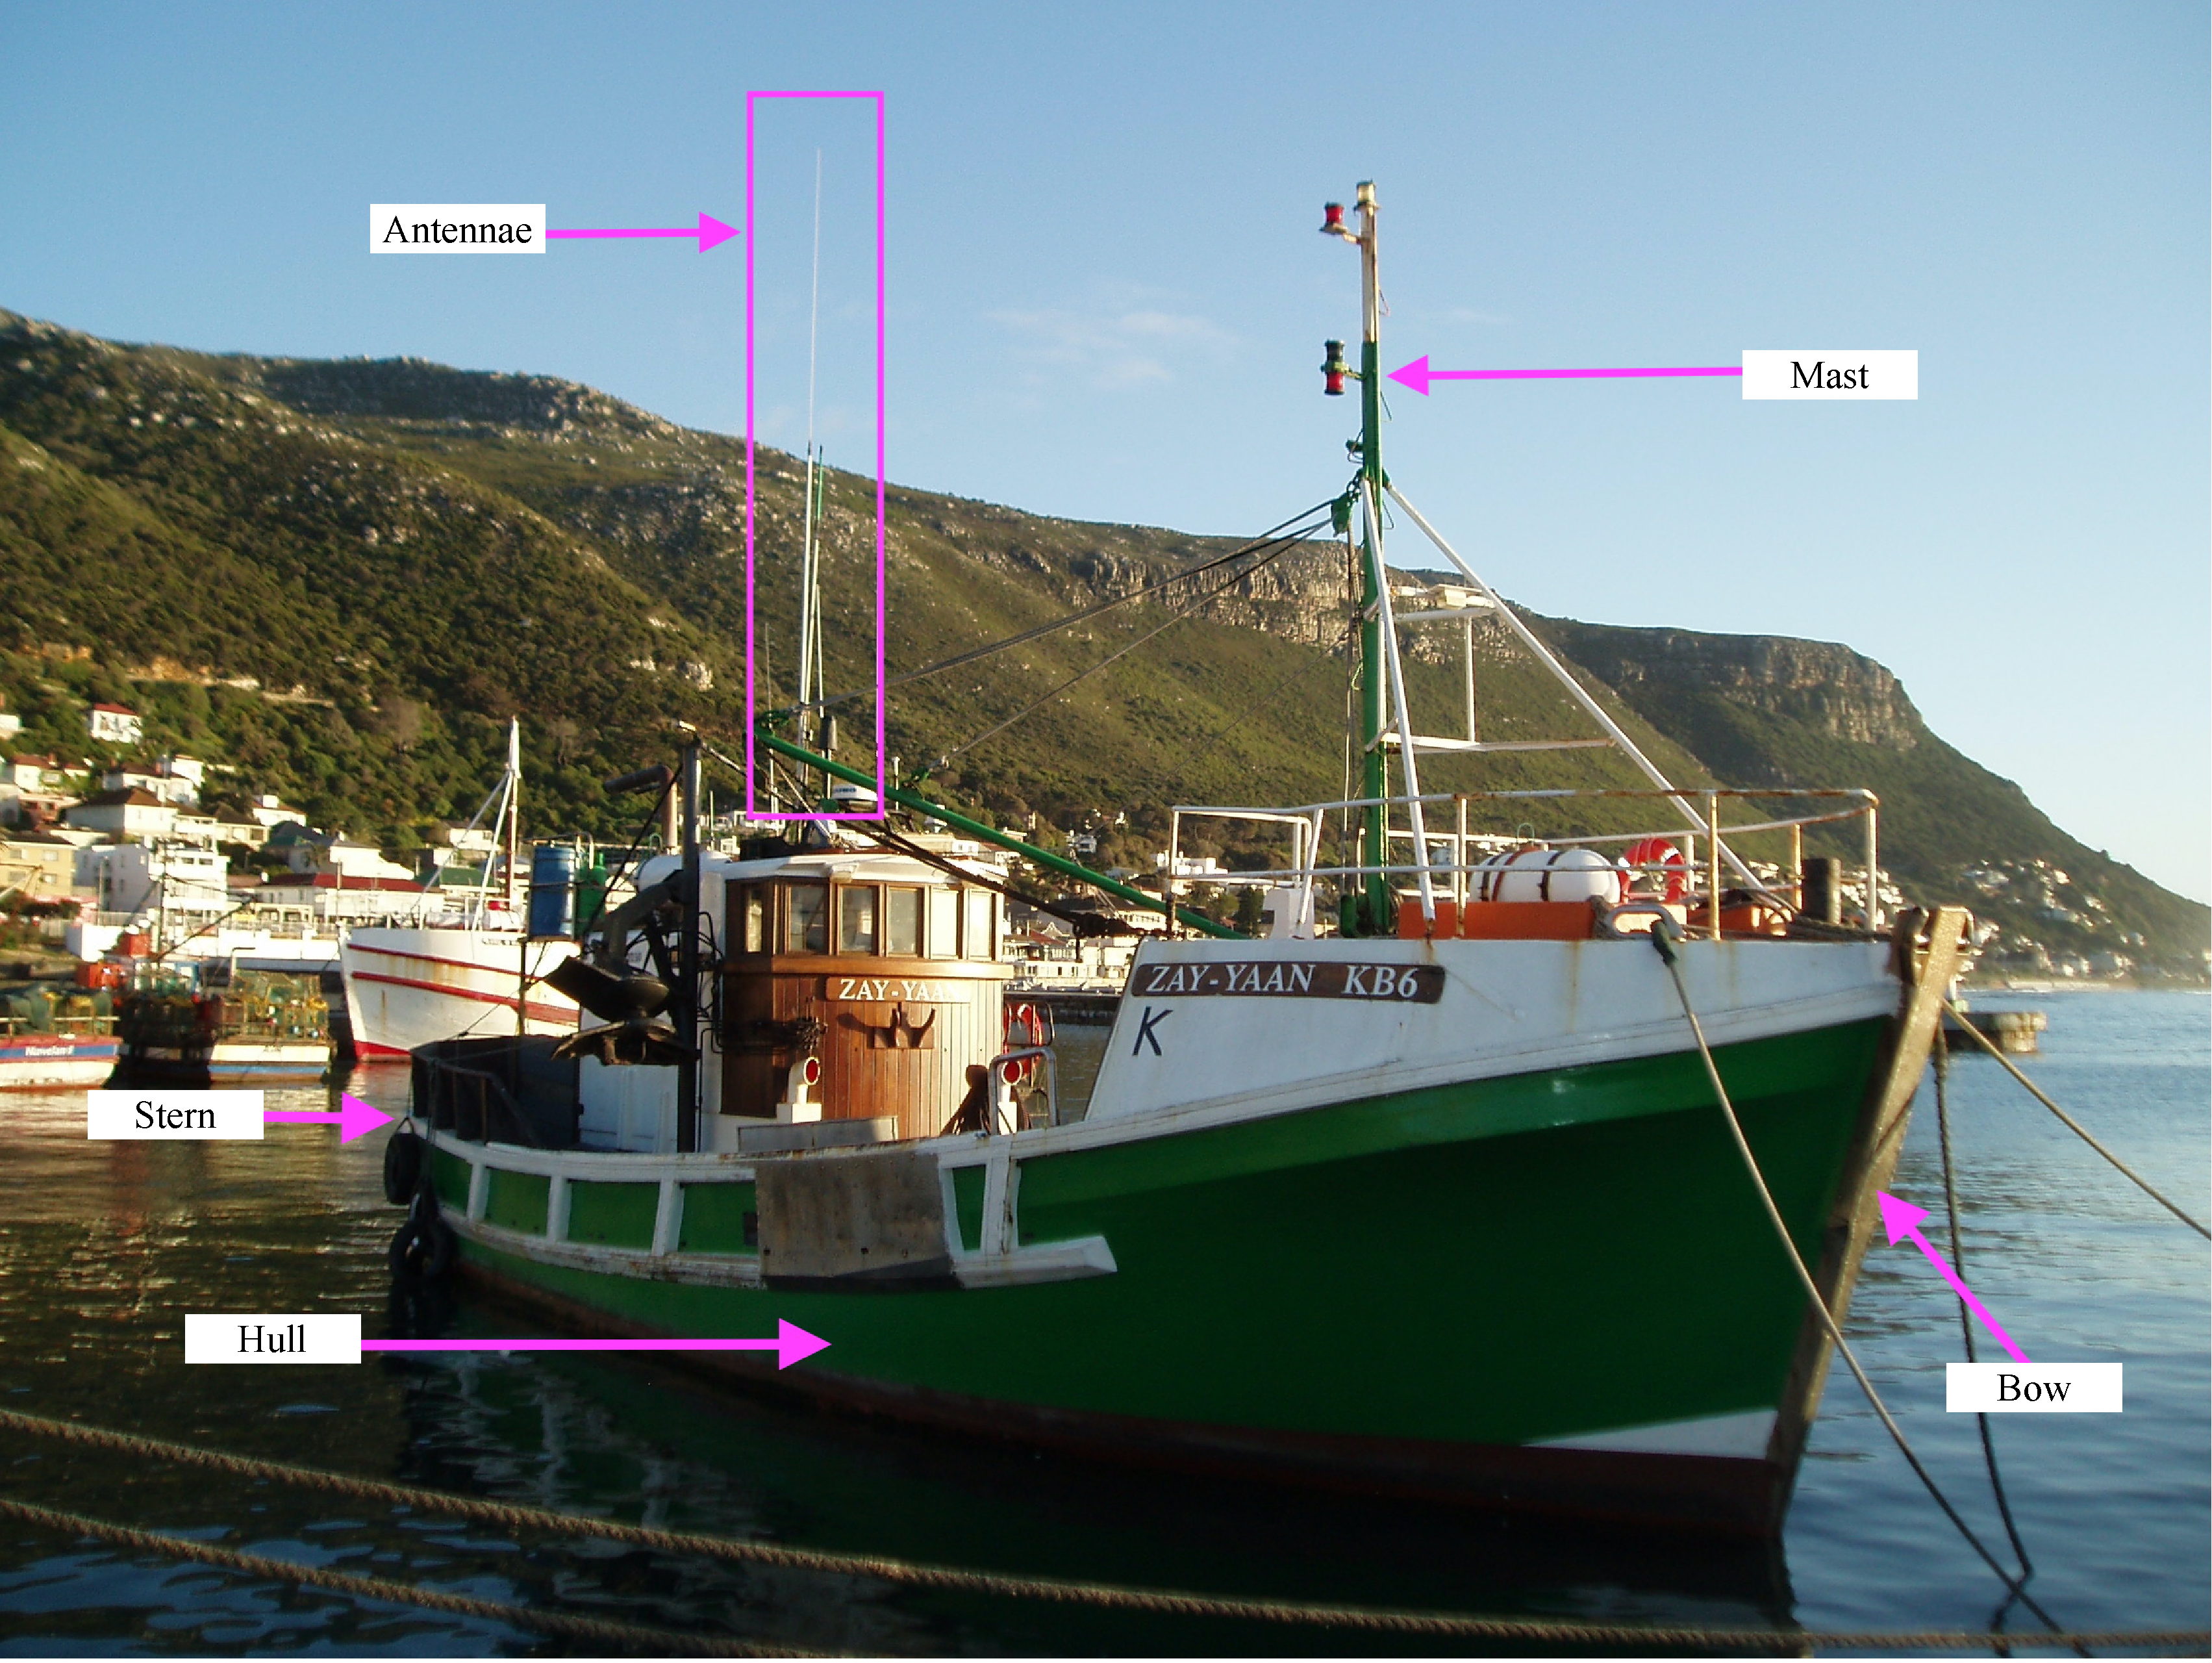
\includegraphics{Figures/04AlgoV&V/Measured/zayyaan.pdf}}
        \caption{Zay-Yaan KB6 boat structure. Adapted from \cite{zayyaan_data}.}
        \label{fig:hayAF_zayyaan}
        \vspace*{-\baselineskip}
    \end{wrapfigure}
    accurate characterisation of the object's features. After \gls{ra}, the antennae were longer and thinner than the mast, and the angular bow was more pronounced. However, there was significant spreading of the object's features over the Doppler axis, which was attributed to the effects of phase errors in the range-aligned profiles and sidelobes in the data. As discussed in \autoref{theory:af}, \gls{af} is used to correct the phase errors introduced by \gls{ra}. \autoref{subfig:hayAF_corrRA_measured_AF_1} shows that after \gls{af} was applied, the Doppler spreading was reduced; however, the shape of the bow and mast were not an accurate representation of the features in \autoref{fig:hayAF_zayyaan}. Notably, the spectral spreading caused by sidelobes was still present as previously discussed. The \gls{ic} values of each image were \textbf{7.0534}, \textbf{8.1803}, and \textbf{10.4345} for the unfocused, range-aligned, and autofocused images, respectively. Although there was a \(\frac{10.4345-7.0534}{7.0534} = 47.94\%\) improvement on the image contrast after \gls{ra} and \gls{af} was applied, the features of the object in \autoref{subfig:hayAF_corrRA_measured_AF_1} were not a satisfactory representation of those in \autoref{fig:hayAF_zayyaan}.

    Importantly, in measured data there often exists more than one \gls{ds}. A limitation of the \gls{sdsaf} algorithm is that it uses only one \gls{ds} to phase correct all profiles. The poor quality of \autoref{subfig:hayAF_corrRA_measured_AF_1} was attributed to the \gls{ds} selected by the \gls{sdsaf} algorithm. As explained in \autoref{theory:noise}, the \gls{snr} of a scatterer is influenced by noise, which subsequently impacts the performance of \gls{af} algorithms. \autoref{fig:hayAF_SCRA_measured_power_1} shows that a low power \gls{ds} was selected when producing \autoref{subfig:hayAF_corrRA_measured_AF_1}. 
    \begin{figure}[H]
        \centering
        \resizebox{0.4\linewidth}{!}{% This file was created by matlab2tikz.
%
%The latest updates can be retrieved from
%  http://www.mathworks.com/matlabcentral/fileexchange/22022-matlab2tikz-matlab2tikz
%where you can also make suggestions and rate matlab2tikz.
%
\definecolor{mycolor1}{rgb}{0.00000,0.44700,0.74100}%
%
\begin{tikzpicture}

\begin{axis}[%
width=6.028in,
height=4.754in,
at={(1.011in,0.642in)},
scale only axis,
xmin=0,
xmax=100,
xlabel style={font=\color{white!15!black}},
xlabel={Range Bin},
ymin=0,
ymax=450000000,
ylabel style={font=\color{white!15!black}},
ylabel={Power},
axis background/.style={fill=white},
title style={font=\bfseries},
title={Power of Scatterers},
legend style={legend cell align=left, align=left, draw=white!15!black}
]
\addplot [color=mycolor1, mark=asterisk, mark options={solid, mycolor1}]
  table[row sep=crcr]{%
1	861234.796275547\\
2	461974.086744226\\
3	212662.339773961\\
4	246092.798143225\\
5	577332.97113036\\
6	729796.050856513\\
7	285852.065768088\\
8	155361.175530255\\
9	136416.432899122\\
10	302947.017025261\\
11	380000.674236901\\
12	179786.527703499\\
13	90055.7061709671\\
14	134545.234798792\\
15	398767.920619562\\
16	294854.48094652\\
17	122705.065492897\\
18	158683.861429191\\
19	408318.951663835\\
20	743554.316483603\\
21	347829.42936103\\
22	213310.002614624\\
23	167223.526227361\\
24	220103.740306779\\
25	394848.395645618\\
26	204227.984290759\\
27	219002.288935564\\
28	190089.498926234\\
29	626846.49285405\\
30	1444945.06603732\\
31	3650263.95712096\\
32	11938621.9610267\\
33	44349992.8398528\\
34	58349363.7747511\\
35	110256789.005583\\
36	86307739.1322255\\
37	21485572.091045\\
38	23974523.3237539\\
39	20142931.4452402\\
40	10755159.5336766\\
41	11884190.0771573\\
42	14600825.1484434\\
43	128804982.972008\\
44	422629109.972909\\
45	154510209.337695\\
46	13638038.8013476\\
47	10474902.5022089\\
48	8795290.35070148\\
49	6149892.63456373\\
50	4530666.55097104\\
51	6218830.29546932\\
52	6627613.6289192\\
53	7702172.06942866\\
54	5670379.25198555\\
55	6029111.47245567\\
56	11146504.1938552\\
57	40973089.3177811\\
58	234197171.492459\\
59	261043993.014117\\
60	94038567.4996435\\
61	81074726.8044155\\
62	21215941.4722665\\
63	16843830.1409221\\
64	37411098.7126583\\
65	33057887.9061113\\
66	15025385.2684402\\
67	7620191.15082092\\
68	27270568.1058131\\
69	28803870.4548784\\
70	16286339.9782475\\
71	7778188.25426342\\
72	4043469.61373697\\
73	2202210.07194016\\
74	884615.743242843\\
75	636807.413944679\\
76	601554.468385522\\
77	547068.603506823\\
78	893601.681393332\\
79	506093.525588289\\
80	247064.291213952\\
81	187083.5266876\\
82	661330.807635752\\
83	688854.084561109\\
84	247028.312680993\\
85	173529.477201299\\
86	277910.276689611\\
87	440341.293104714\\
88	365167.084965798\\
89	162743.493973739\\
90	114180.84957851\\
91	243478.842305658\\
92	443347.004440988\\
93	394435.59230442\\
94	207066.130743798\\
95	204547.634516275\\
96	432162.614055562\\
};
\addlegendentry{Scatterer power}

\addplot [color=orange]
  table[row sep=crcr]{%
0	22499787.3670263\\
100	22499787.3670263\\
};
\addlegendentry{Average power of all scatterers}

\addplot [color=black, only marks, mark size=4.0pt, mark=o, mark options={solid, black}]
  table[row sep=crcr]{%
33	44349992.8398528\\
34	58349363.7747511\\
35	110256789.005583\\
36	86307739.1322255\\
38	23974523.3237539\\
43	128804982.972008\\
44	422629109.972909\\
45	154510209.337695\\
57	40973089.3177811\\
58	234197171.492459\\
59	261043993.014117\\
60	94038567.4996435\\
61	81074726.8044155\\
64	37411098.7126583\\
65	33057887.9061113\\
68	27270568.1058131\\
69	28803870.4548784\\
};
\addlegendentry{Candidate scatterers}

\addplot [color=red, only marks, mark size=7.5pt, mark=o, mark options={solid, red}]
  table[row sep=crcr]{%
65	33057887.9061113\\
};
\addlegendentry{Dominant scatterer}

\end{axis}

\begin{axis}[%
width=7.778in,
height=5.833in,
at={(0in,0in)},
scale only axis,
xmin=0,
xmax=1,
ymin=0,
ymax=1,
axis line style={draw=none},
ticks=none,
axis x line*=bottom,
axis y line*=left
]
\end{axis}
\end{tikzpicture}%}
        \caption{Scatterer power for the selection of a \gls{ds} in \gls{sdsaf} applied to correlation range-aligned measured \gls{hrr} profiles}
       \label{fig:hayAF_SCRA_measured_power_1}
    \end{figure}

    Consequently, whilst multiple \gls{ds}s cannot be selected, a different approach was taken to improve the performance of the algorithm. A \gls{sf} was introduced into line 10 of \autoref{alg:haywood_AF} to ensure that a higher power \gls{ds} was selected. The aim was to improve the quality of the autofocused image by selecting a \gls{ds} that was less affected by noise. This was implemented as shown in \autoref{code:scaling_factor}.
% !!!!!!!!!!!!!! DO NOT INDENT IT MESSES UP THE LATEX !!!!!!!!!!!!!!!!!!!!!!!!!!!!!!!!!
\begin{lstlisting}[caption={\textsc{MATLAB} code for scaling factor in candidate \gls{ds} selection.},label={code:scaling_factor}]
scaling_factor = 10;
candidate_scatterers_idx = find(power_scatterer>scaling_factor*average_power_scatterer);
\end{lstlisting}

    Two scaling factors, namely 5 and 10, were used to test the effect of the improved implementation on the performance of \gls{sdsaf}. \autoref{subfig:hayAF_SCRA_measured_power_sf5} and \autoref{subfig:hayAF_SCRA_measured_power_sf10} show that as the \gls{sf} increased, a higher power \gls{ds} was selected as expected.
    \begin{figure}[H]
        \centering
        \begin{subfigure}{0.4\linewidth}
            \resizebox{\linewidth}{!}{% This file was created by matlab2tikz.
%
%The latest updates can be retrieved from
%  http://www.mathworks.com/matlabcentral/fileexchange/22022-matlab2tikz-matlab2tikz
%where you can also make suggestions and rate matlab2tikz.
%
\definecolor{mycolor1}{rgb}{0.00000,0.44700,0.74100}%
%
\begin{tikzpicture}

\begin{axis}[%
width=6.028in,
height=4.754in,
at={(1.011in,0.642in)},
scale only axis,
xmin=0,
xmax=100,
xlabel style={font=\color{white!15!black}},
xlabel={Range Bin},
ymin=0,
ymax=450000000,
ylabel style={font=\color{white!15!black}},
ylabel={Power},
axis background/.style={fill=white},
legend style={legend cell align=left, align=left, draw=white!15!black}
]
\addplot [color=mycolor1, mark=asterisk, mark options={solid, mycolor1}]
  table[row sep=crcr]{%
1	861234.796275547\\
2	461974.086744226\\
3	212662.339773961\\
4	246092.798143225\\
5	577332.97113036\\
6	729796.050856513\\
7	285852.065768088\\
8	155361.175530255\\
9	136416.432899122\\
10	302947.017025261\\
11	380000.674236901\\
12	179786.527703499\\
13	90055.7061709671\\
14	134545.234798792\\
15	398767.920619562\\
16	294854.48094652\\
17	122705.065492897\\
18	158683.861429191\\
19	408318.951663835\\
20	743554.316483603\\
21	347829.42936103\\
22	213310.002614624\\
23	167223.526227361\\
24	220103.740306779\\
25	394848.395645618\\
26	204227.984290759\\
27	219002.288935564\\
28	190089.498926234\\
29	626846.49285405\\
30	1444945.06603732\\
31	3650263.95712096\\
32	11938621.9610267\\
33	44349992.8398528\\
34	58349363.7747511\\
35	110256789.005583\\
36	86307739.1322255\\
37	21485572.091045\\
38	23974523.3237539\\
39	20142931.4452402\\
40	10755159.5336766\\
41	11884190.0771573\\
42	14600825.1484434\\
43	128804982.972008\\
44	422629109.972909\\
45	154510209.337695\\
46	13638038.8013476\\
47	10474902.5022089\\
48	8795290.35070148\\
49	6149892.63456373\\
50	4530666.55097104\\
51	6218830.29546932\\
52	6627613.6289192\\
53	7702172.06942866\\
54	5670379.25198555\\
55	6029111.47245567\\
56	11146504.1938552\\
57	40973089.3177811\\
58	234197171.492459\\
59	261043993.014117\\
60	94038567.4996435\\
61	81074726.8044155\\
62	21215941.4722665\\
63	16843830.1409221\\
64	37411098.7126583\\
65	33057887.9061113\\
66	15025385.2684402\\
67	7620191.15082092\\
68	27270568.1058131\\
69	28803870.4548784\\
70	16286339.9782475\\
71	7778188.25426342\\
72	4043469.61373697\\
73	2202210.07194016\\
74	884615.743242843\\
75	636807.413944679\\
76	601554.468385522\\
77	547068.603506823\\
78	893601.681393332\\
79	506093.525588289\\
80	247064.291213952\\
81	187083.5266876\\
82	661330.807635752\\
83	688854.084561109\\
84	247028.312680993\\
85	173529.477201299\\
86	277910.276689611\\
87	440341.293104714\\
88	365167.084965798\\
89	162743.493973739\\
90	114180.84957851\\
91	243478.842305658\\
92	443347.004440988\\
93	394435.59230442\\
94	207066.130743798\\
95	204547.634516275\\
96	432162.614055562\\
};
\addlegendentry{Scatterer power}

\addplot [color=orange]
  table[row sep=crcr]{%
0	112498936.835131\\
100	112498936.835131\\
};
\addlegendentry{Average power of all scatterers}

\addplot [color=black, only marks, mark size=4.0pt, mark=o, mark options={solid, black}]
  table[row sep=crcr]{%
43	128804982.972008\\
44	422629109.972909\\
45	154510209.337695\\
58	234197171.492459\\
59	261043993.014117\\
};
\addlegendentry{Candidate scatterers}

\addplot [color=red, only marks, mark size=7.5pt, mark=o, mark options={solid, red}]
  table[row sep=crcr]{%
43	128804982.972008\\
};
\addlegendentry{Dominant scatterer}

\end{axis}

\begin{axis}[%
width=7.778in,
height=5.833in,
at={(0in,0in)},
scale only axis,
xmin=0,
xmax=1,
ymin=0,
ymax=1,
axis line style={draw=none},
ticks=none,
axis x line*=bottom,
axis y line*=left
]
\end{axis}
\end{tikzpicture}%}
            \caption{\gls{sf} = 5. \label{subfig:hayAF_SCRA_measured_power_sf5}}
        \end{subfigure}
        \hspace{0.5cm}
        \begin{subfigure}{0.4\linewidth}
            \resizebox{\linewidth}{!}{% This file was created by matlab2tikz.
%
%The latest updates can be retrieved from
%  http://www.mathworks.com/matlabcentral/fileexchange/22022-matlab2tikz-matlab2tikz
%where you can also make suggestions and rate matlab2tikz.
%
\definecolor{mycolor1}{rgb}{0.00000,0.44700,0.74100}%
%
\begin{tikzpicture}

\begin{axis}[%
width=6.028in,
height=4.754in,
at={(1.011in,0.642in)},
scale only axis,
xmin=0,
xmax=100,
xlabel style={font=\color{white!15!black}},
xlabel={Range Bin},
ymin=0,
ymax=450000000,
ylabel style={font=\color{white!15!black}},
ylabel={Power},
axis background/.style={fill=white},
title style={font=\bfseries},
title={Power of Scatterers},
legend style={legend cell align=left, align=left, draw=white!15!black}
]
\addplot [color=mycolor1, mark=asterisk, mark options={solid, mycolor1}]
  table[row sep=crcr]{%
1	861234.796275547\\
2	461974.086744226\\
3	212662.339773961\\
4	246092.798143225\\
5	577332.97113036\\
6	729796.050856513\\
7	285852.065768088\\
8	155361.175530255\\
9	136416.432899122\\
10	302947.017025261\\
11	380000.674236901\\
12	179786.527703499\\
13	90055.7061709671\\
14	134545.234798792\\
15	398767.920619562\\
16	294854.48094652\\
17	122705.065492897\\
18	158683.861429191\\
19	408318.951663835\\
20	743554.316483603\\
21	347829.42936103\\
22	213310.002614624\\
23	167223.526227361\\
24	220103.740306779\\
25	394848.395645618\\
26	204227.984290759\\
27	219002.288935564\\
28	190089.498926234\\
29	626846.49285405\\
30	1444945.06603732\\
31	3650263.95712096\\
32	11938621.9610267\\
33	44349992.8398528\\
34	58349363.7747511\\
35	110256789.005583\\
36	86307739.1322255\\
37	21485572.091045\\
38	23974523.3237539\\
39	20142931.4452402\\
40	10755159.5336766\\
41	11884190.0771573\\
42	14600825.1484434\\
43	128804982.972008\\
44	422629109.972909\\
45	154510209.337695\\
46	13638038.8013476\\
47	10474902.5022089\\
48	8795290.35070148\\
49	6149892.63456373\\
50	4530666.55097104\\
51	6218830.29546932\\
52	6627613.6289192\\
53	7702172.06942866\\
54	5670379.25198555\\
55	6029111.47245567\\
56	11146504.1938552\\
57	40973089.3177811\\
58	234197171.492459\\
59	261043993.014117\\
60	94038567.4996435\\
61	81074726.8044155\\
62	21215941.4722665\\
63	16843830.1409221\\
64	37411098.7126583\\
65	33057887.9061113\\
66	15025385.2684402\\
67	7620191.15082092\\
68	27270568.1058131\\
69	28803870.4548784\\
70	16286339.9782475\\
71	7778188.25426342\\
72	4043469.61373697\\
73	2202210.07194016\\
74	884615.743242843\\
75	636807.413944679\\
76	601554.468385522\\
77	547068.603506823\\
78	893601.681393332\\
79	506093.525588289\\
80	247064.291213952\\
81	187083.5266876\\
82	661330.807635752\\
83	688854.084561109\\
84	247028.312680993\\
85	173529.477201299\\
86	277910.276689611\\
87	440341.293104714\\
88	365167.084965798\\
89	162743.493973739\\
90	114180.84957851\\
91	243478.842305658\\
92	443347.004440988\\
93	394435.59230442\\
94	207066.130743798\\
95	204547.634516275\\
96	432162.614055562\\
};
\addlegendentry{Scatterer power}

\addplot [color=orange]
  table[row sep=crcr]{%
0	224997873.670263\\
100	224997873.670263\\
};
\addlegendentry{Average power of all scatterers}

\addplot [color=black, only marks, mark size=4.0pt, mark=o, mark options={solid, black}]
  table[row sep=crcr]{%
44	422629109.972909\\
58	234197171.492459\\
59	261043993.014117\\
};
\addlegendentry{Candidate scatterers}

\addplot [color=red, only marks, mark size=7.5pt, mark=o, mark options={solid, red}]
  table[row sep=crcr]{%
59	261043993.014117\\
};
\addlegendentry{Dominant scatterer}

\end{axis}

\begin{axis}[%
width=7.778in,
height=5.833in,
at={(0in,0in)},
scale only axis,
xmin=0,
xmax=1,
ymin=0,
ymax=1,
axis line style={draw=none},
ticks=none,
axis x line*=bottom,
axis y line*=left
]
\end{axis}
\end{tikzpicture}%}
            \caption{\gls{sf} = 10. \label{subfig:hayAF_SCRA_measured_power_sf10}}
        \end{subfigure}
        \caption{Scatterer power for the selection of a \gls{ds} in \gls{sdsaf} using various threshold \gls{sf}s applied to correlation range-aligned measured \gls{hrr} profiles} \label{fig:hayAF_SCRA_measured_power_2}
    \end{figure}

    Subsequently, introducing the \gls{sf} produced the images in \autoref{subfig:hayAF_corrRA_measured_2}. \autoref{subfig:hayAF_corrRA_measured_SF1} shows the focused image before the \gls{sf} was introduced which inherently means that the \gls{sf} was 1. The \gls{ic} values for each image were calculated to provide a quantitative evaluation of the \gls{sf}'s effect on the performance of \gls{sdsaf}. The values for images (a),(b) and (c) in \autoref{subfig:hayAF_corrRA_measured_2} were calculated as \textbf{10.4345}, \textbf{15.1049} and \textbf{15.2911} respectively. The improvement of the \gls{ic} values as the \gls{sf} increased, indicated that introducing the \gls{sf} improved the performance of \gls{sdsaf}.
    
    Although the \gls{ic} values indicated that \autoref{subfig:hayAF_corrRA_measured_SF5} and \autoref{subfig:hayAF_corrRA_measured_SF10} were similarly focused, the visual results did not reflect his result. In \autoref{subfig:hayAF_corrRA_measured_SF5}, the Doppler spreading, was reduced compared to \autoref{subfig:hayAF_corrRA_measured_SF1} however, the features of the boat were less recognisable. Whilst the antennae were well represented as a long, thin regtangular cluster, the bow and stern were taller than expected. In contrast, when a \gls{sf} of 10 was used, \autoref{subfig:hayAF_corrRA_measured_SF5} showed the most accurate representation of the boat's features. There was a distinct long, thin rectangular cluster of scatterers representing the antennae and the angular bow and round stern were clearly identifiable. Additionally, there was a clear cluster of scatterers at the bow of the ship which accurately represented the front end of the ship shown in \autoref{fig:zayyaan}.

    \begin{figure}[H]
        \centering
        \begin{subfigure}{0.3\linewidth}
            \resizebox{\linewidth}{!}{% This file was created by matlab2tikz.
%
%The latest updates can be retrieved from
%  http://www.mathworks.com/matlabcentral/fileexchange/22022-matlab2tikz-matlab2tikz
%where you can also make suggestions and rate matlab2tikz.
%
\begin{tikzpicture}
\begin{axis}[%
width=5.554in,
height=4.754in,
at={(0.932in,0.642in)},
scale only axis,
point meta min=-40,
point meta max=0,
axis on top,
xmin=0,
xmax=29.6578125,
xlabel style={font=\fontsize{25}{14}\selectfont\color{black}, yshift=-10pt},
xlabel={Range (m)},
ymin=-88.0034,
ymax=86.6175,
ylabel style={font=\fontsize{25}{14}\selectfont\color{black}},
ylabel={Doppler frquency (Hz)},
axis background/.style={fill=white},
tick label style={font=\fontsize{20}{11}\selectfont\color{black}},
xtick distance= 4,             % Set the spacing between x-axis ticks
ytick distance = 10,
colormap/jet,
colorbar
]
\addplot [forget plot] graphics [xmin=0, xmax=29.6578125, ymin=-88.0034, ymax=86.6175] {Figures/04AlgoV&V/Measured/04HayAF/CorrRA/HayAF_SCRA_Measured_ISAR.png};
\end{axis}

\end{tikzpicture}%}
            \caption{\gls{sf} = 1. \label{subfig:hayAF_corrRA_measured_SF1}}
        \end{subfigure}
        \hspace{0.5cm}
        \begin{subfigure}{0.3\linewidth}
            \resizebox{\linewidth}{!}{% This file was created by matlab2tikz.
%
%The latest updates can be retrieved from
%  http://www.mathworks.com/matlabcentral/fileexchange/22022-matlab2tikz-matlab2tikz
%where you can also make suggestions and rate matlab2tikz.
%
\begin{tikzpicture}
\begin{axis}[%
width=5.554in,
height=4.754in,
at={(0.932in,0.642in)},
scale only axis,
point meta min=-40,
point meta max=0,
axis on top,
xmin=0,
xmax=29.6578125,
xlabel style={font=\fontsize{25}{14}\selectfont\color{black}, yshift=-10pt},
xlabel={Range (m)},
ymin=-88.0034,
ymax=86.6175,
ylabel style={font=\fontsize{25}{14}\selectfont\color{black}},
ylabel={Doppler frquency (Hz)},
axis background/.style={fill=white},
tick label style={font=\fontsize{20}{11}\selectfont\color{black}},
xtick distance= 4,             % Set the spacing between x-axis ticks
ytick distance = 10,
colormap/jet,
colorbar
]
\addplot [forget plot] graphics [xmin=0, xmax=29.6578125, ymin=-88.0034, ymax=86.6175] {Figures/04AlgoV&V/Measured/04HayAF/ScalingFactor/ISAR/HayAF_SCRA_Measured_ISAR_SF5.png};
\end{axis}

\end{tikzpicture}%}
            \caption{\gls{sf} = 5. \label{subfig:hayAF_corrRA_measured_SF5}}
        \end{subfigure}
        \hspace{0.5cm}
        \begin{subfigure}{0.3\linewidth}
            \resizebox{\linewidth}{!}{% This file was created by matlab2tikz.
%
%The latest updates can be retrieved from
%  http://www.mathworks.com/matlabcentral/fileexchange/22022-matlab2tikz-matlab2tikz
%where you can also make suggestions and rate matlab2tikz.
%
\begin{tikzpicture}
\begin{axis}[%
width=5.554in,
height=4.754in,
at={(0.932in,0.642in)},
scale only axis,
point meta min=-40,
point meta max=0,
axis on top,
xmin=0,
xmax=29.6578125,
xlabel style={font=\fontsize{25}{14}\selectfont\color{black}, yshift=-10pt},
xlabel={Range (m)},
ymin=-88.0034,
ymax=86.6175,
ylabel style={font=\fontsize{25}{14}\selectfont\color{black}},
ylabel={Doppler frquency (Hz)},
axis background/.style={fill=white},
tick label style={font=\fontsize{20}{11}\selectfont\color{black}},
xtick distance= 4,             % Set the spacing between x-axis ticks
ytick distance = 10,
colormap/jet,
colorbar
]
\addplot [forget plot] graphics [xmin=0, xmax=29.6578125, ymin=-88.0034, ymax=86.6175] {Figures/04AlgoV&V/Measured/04HayAF/ScalingFactor/ISAR/HayAF_SCRA_Measured_ISAR_SF10.png};
\end{axis}

\end{tikzpicture}%}
            \caption{\gls{sf} = 10.\label{subfig:hayAF_corrRA_measured_SF10}}
        \end{subfigure}
        \caption{\gls{isar} images of after \gls{sdsaf} using different scaling factors applied to Correlation range-aligned measured \gls{hrr} profiles.} \label{subfig:hayAF_corrRA_measured_2}
    \end{figure}

    Therefore, the \gls{sf} improved the performance of \gls{sdsaf}, resulting in a more focused image. Using a \gls{sf} of 10 produced an image which more accurately represented the features on the boat than the image produced when no \gls{sf} was used. However, when a scaling factor of 5 was used, the image appeared less focused. This was attributed to the selection of an unsuitable \gls{ds}. Importantly, this does not imply that a \gls{sf} of 5 is inherently less desirable than a \gls{sf} of 1. Rather, it was a consequence of the characteristics of the dataset and could occur regardless of the chosen \gls{sf}. 

    Overall, the improved \gls{sdsaf} implementation produced a focused \gls{isar} image when using a \gls{sf} of 10 and was validated for use in this report. This \gls{sf} of 10 was used for all following experimentation which involved \gls{sdsaf}.

%%%%%%%%%%%%%%%%%%%%%%%%%%%%%%%%%%%%%%%%%%%%%%%%%%%%%%%%%%%%%%%%%%%%%%%%%%%%%%%%%%%%%%%%%%%%%%%%%%%%
\section{Multiple Dominant Scatterer Autofocus Algorithm}\label{subsec:yuanAF}
The \gls{mdsaf} algorithm is a type of \gls{dsa} that uses a set of scatterers to phase correct \gls{hrr} profiles. The \gls{ds}s are selected as those with the least dispersion\footnote{Dispersion describes the spread of the scatterer across all \gls{hrr} profiles}. The \gls{mdsaf} algorithm, as described in \cite{yuan_AF}, was outlined in \autoref{alg:yuan_AF}.
 
    %***************************************************************************************%
    \subsection{Pseudo Code and Implementation}
    % Yuan AF Pseudo code
    \begin{figure}[H]
        \vspace{0.25cm}
        \centering
        \captionsetup{type=figure}
        \begin{minipage}{.8\linewidth}
            \begin{algorithm}[H]
            \caption{Haywood \gls{ra} Algorithm.\label{alg:yuan_AF}}
        
            \LinesNumbered % NUMBER THE LINES
            \DontPrintSemicolon
            \SetAlgoLined
            \SetKwInOut{Input}{input}\SetKwInOut{Output}{output}\SetKwInOut{Parameter}{parameter}
        
            \Input{All \gls{hrrp}s, matrix $hrrp_{all}$}
            \Output{Range-aligned \gls{hrrp}s, matrix $hrrp_{RA}$}
            \Parameter{Reference \gls{hrrp} number, $refIndex$}
        
            \BlankLine
            \Begin{
                $scattererAmplitudes \leftarrow 0$\;
               \For(){$k$ in 1 to rows($hrrp_{RA}$)}{
                    \For(){$n$ in 1 to $columns(hrrp_{RA})$}{
                        $scattererAmplitudes \leftarrow scattererAmplitudes + |hrrp_{RA}[k][n]|^2 $\;
                    }
                    $mean[n] \leftarrow mean(scattererAmplitudes) $\;
                    $variance[n] \leftarrow var(scattererAmplitudes) $\;
                }

                $a \leftarrow 0$\;
                \For(){$b$ in 1 to length($mean$)}{
                    $dispersion[b] \leftarrow variance[b]/(variance[b] + mean[b]^2)$\;
                    \If{$dispersion>0.16$}{
                        $candidateIndices[a] \leftarrow b$\;
                        $a \leftarrow a + 1$\;
                    } 
                }
                $candidateIndices_{sorted} \leftarrow$ indices of ascending sort $dispersion(candidateIndices)$\;
                \gls{ds}$indices \leftarrow candidateIndices_{sorted}[1$ to $11]$\;
                \For(){$b$ in 1 to length(\gls{ds}$indices$)}{
                    \For(){$k$ in 1 to rows($hrrp_{RA}$)}{
                        $product[k][b] = conjugate(hrrp_{RA}[refIndex][b]) \cdot hrrp_{RA}[k][b] $\;
                    }
                }
                \For(){$k$ in 1 to rows($product$)}{
                    $angle \leftarrow angle(mean(product[k]))$\;
                    $phaseShift[k] \leftarrow exp(-1i \cdot angle)$
                }
                \For(){$k$ in 1 to rows($hrrp_{RA}$)}{
                    \For(){$n$ in 1 to $columns(hrrp_{RA})$}{
                        $hrrp_{AF}[k][n] \leftarrow hrrp_{RA}[k][n] \cdot phaseShift[k] $
                    }
                }
            }
          \vspace{0.25cm}
        \end{algorithm}
      \end{minipage}
    \end{figure}

    The \gls{mdsaf} algorithm was implemented as a stand-alone \textsc{MATLAB} function. The implemented function, \href{}{yuanAF.m}, was validated and verified in this section.
    %***************************************************************************************%
    \subsection{Algorithm Verification}
    Correlation range-aligned simulated \gls{hrr} profiles were used to verify that \autoref{alg:yuan_AF} was implemented correctly in \textsc{MATLAB}.
    
    \begin{figure}[H]
        \centering
        \resizebox{0.45\linewidth}{!}{% This file was created by matlab2tikz.
%
%The latest updates can be retrieved from
%  http://www.mathworks.com/matlabcentral/fileexchange/22022-matlab2tikz-matlab2tikz
%where you can also make suggestions and rate matlab2tikz.
%
\definecolor{mycolor1}{rgb}{0.00000,0.44700,0.74100}%
%
\begin{tikzpicture}

\begin{axis}[%
width=6.028in,
height=4.754in,
at={(1.011in,0.642in)},
scale only axis,
xmin=0,
xmax=256,
xlabel style={font=\color{white!15!black}},
xlabel={Range Bin Number},
ymin=0,
ymax=0.5,
ylabel style={font=\color{white!15!black}},
ylabel={Scatterer Dispersion},
axis background/.style={fill=white},
scaled y ticks=base 10:2,
legend style={legend cell align=left, align=left, draw=white!15!black},
grid=both,  % Enables major grids
minor tick num=10,  % Sets the number of minor grid lines between major lines
grid style={dashed,gray!50},  % Style for major grids
minor grid style={dotted,gray!50} % Style for minor grids
]
\addplot [color=mycolor1, mark=asterisk, mark options={solid, mycolor1}]
  table[row sep=crcr]{%
1	0.242472205217314\\
2	0.228281680133261\\
3	0.231867172082767\\
4	0.228775674189814\\
5	0.23464878333725\\
6	0.233684497631805\\
7	0.237893676771172\\
8	0.233454924867458\\
9	0.233326386311942\\
10	0.231932030869612\\
11	0.234228631756231\\
12	0.229842334073289\\
13	0.225779380733206\\
14	0.236329732203914\\
15	0.225816565245521\\
16	0.216822562098859\\
17	0.233145224088875\\
18	0.23217811901606\\
19	0.234993965750433\\
20	0.235859973978951\\
21	0.226765218407584\\
22	0.247921923456442\\
23	0.234597113225547\\
24	0.232588695232995\\
25	0.237919910277263\\
26	0.229533102700051\\
27	0.238780503823198\\
28	0.241787608706607\\
29	0.229596968240643\\
30	0.236801410503842\\
31	0.228106913500198\\
32	0.228400631086744\\
33	0.237057297145007\\
34	0.221898331936325\\
35	0.227875425095176\\
36	0.234329704994029\\
37	0.231380518743503\\
38	0.219303125480171\\
39	0.224549022289551\\
40	0.224769369624797\\
41	0.229650852349172\\
42	0.230733599999139\\
43	0.226443942847752\\
44	0.222394278823108\\
45	0.219042430421739\\
46	0.218558490604716\\
47	0.209642279097181\\
48	0.227668896325328\\
49	0.210325848634692\\
50	0.2053955114873\\
51	0.203772134745206\\
52	0.199333180186502\\
53	0.187484706860977\\
54	0.185402187726268\\
55	0.178709390577263\\
56	0.185260232471041\\
57	0.220905162097239\\
58	0.370968488963322\\
59	0.0289303355595124\\
60	0.227970227818047\\
61	0.161322424091703\\
62	0.152463234748674\\
63	0.167659423566796\\
64	0.20590533514098\\
65	0.38612766823177\\
66	0.0937365632924775\\
67	0.140945969418004\\
68	0.111889092323688\\
69	0.100784436936498\\
70	0.114999411585905\\
71	0.160162574209326\\
72	0.293222653477795\\
73	0.207303431433959\\
74	0.207639132730067\\
75	0.197238489537171\\
76	0.197433177941712\\
77	0.199927007198841\\
78	0.188629440649179\\
79	0.142414806679571\\
80	0.311817640521416\\
81	0.187670721484078\\
82	0.184106324395026\\
83	0.209789732481713\\
84	0.212946974703568\\
85	0.205126326259905\\
86	0.0581494846332972\\
87	0.357520544664959\\
88	0.275557589628519\\
89	0.289410098276132\\
90	0.257426154413877\\
91	0.21145629399713\\
92	0.302771518734655\\
93	0.0219589657442006\\
94	0.300759614620267\\
95	0.226083722192232\\
96	0.209455309084562\\
97	0.197648774865582\\
98	0.185896767812167\\
99	0.343891576282424\\
100	0.0362616501041142\\
101	0.0942409855812491\\
102	0.0611214936583683\\
103	0.0723897025212124\\
104	0.105214261266935\\
105	0.195567642788944\\
106	0.32738415803834\\
107	0.445157198740854\\
108	0.361740088708386\\
109	0.288226768263629\\
110	0.185655340762208\\
111	0.113426808252149\\
112	0.0786262475796283\\
113	0.284385059709277\\
114	0.257702818228682\\
115	0.171250688881076\\
116	0.155516967808048\\
117	0.150093565502611\\
118	0.13855628680634\\
119	0.12287471008334\\
120	0.0288547944841395\\
121	0.177828531118732\\
122	0.122030409190687\\
123	0.132892894567406\\
124	0.139308286522478\\
125	0.147464481906852\\
126	0.206610226052194\\
127	0.0307897653287673\\
128	0.341963722974923\\
129	0.227452362873925\\
130	0.203644831017871\\
131	0.193602372188\\
132	0.180872203076216\\
133	0.142835870142669\\
134	0.0100156959522264\\
135	0.195430849539596\\
136	0.169114348260267\\
137	0.175018101234761\\
138	0.180626500418335\\
139	0.183607831819772\\
140	0.318223997655442\\
141	0.111581548335891\\
142	0.126469393267596\\
143	0.132918493756276\\
144	0.156504682764636\\
145	0.180197399821355\\
146	0.231815762311855\\
147	0.330804596108636\\
148	0.454648539271111\\
149	0.441450313730432\\
150	0.396818621037509\\
151	0.333367297196587\\
152	0.267777223710883\\
153	0.189890475514711\\
154	0.149718607674286\\
155	0.256352537885644\\
156	0.18702167687421\\
157	0.180448395459312\\
158	0.180773961421034\\
159	0.174895065804231\\
160	0.151566081229615\\
161	0.0535988422408038\\
162	0.343921535183397\\
163	0.221514160217016\\
164	0.254401560766594\\
165	0.263857532214145\\
166	0.230549786049896\\
167	0.255249728408107\\
168	0.0265727358298932\\
169	0.336630970867553\\
170	0.252682408432889\\
171	0.22142928568783\\
172	0.208119263005641\\
173	0.230742339195327\\
174	0.382712561292207\\
175	0.028930305134853\\
176	0.186229292767029\\
177	0.134448680881612\\
178	0.133353239137988\\
179	0.136167277670959\\
180	0.176034304145401\\
181	0.36212657846718\\
182	0.0940660152368044\\
183	0.154232280126883\\
184	0.146471856590351\\
185	0.148736107544247\\
186	0.168091116462152\\
187	0.201801119430621\\
188	0.290133245429613\\
189	0.217266669735228\\
190	0.186382909293824\\
191	0.163575356653549\\
192	0.159550231613122\\
193	0.159843373717936\\
194	0.151317825487919\\
195	0.143026220152161\\
196	0.313501210154127\\
197	0.216817705114098\\
198	0.207098118116082\\
199	0.208756340965032\\
200	0.230772059728579\\
201	0.240927334163293\\
202	0.249267848775455\\
203	0.268095915875369\\
204	0.268892382836204\\
205	0.29545615467547\\
206	0.295810330467397\\
207	0.308180394647989\\
208	0.297151656960574\\
209	0.301103428787389\\
210	0.300906970850329\\
211	0.295737085843697\\
212	0.298733154714701\\
213	0.30172333845887\\
214	0.287747828223305\\
215	0.281871527440154\\
216	0.275300161428793\\
217	0.280357424776904\\
218	0.281093354293528\\
219	0.266768550164441\\
220	0.272832854088091\\
221	0.269565051889486\\
222	0.269012671554915\\
223	0.270337036688436\\
224	0.266573723338601\\
225	0.26060581095721\\
226	0.25858910852522\\
227	0.247779657962507\\
228	0.251670613641895\\
229	0.263575998169665\\
230	0.262167290684185\\
231	0.26151225106329\\
232	0.25537192703796\\
233	0.259133697441164\\
234	0.247508066403123\\
235	0.254948069023678\\
236	0.258459453111456\\
237	0.248504831530959\\
238	0.252989818827077\\
239	0.24780379641046\\
240	0.248815297157452\\
241	0.251570682327941\\
242	0.232846155682828\\
243	0.24139138966315\\
244	0.241416290377392\\
245	0.24937004708173\\
246	0.238255146349482\\
247	0.260105540504784\\
248	0.237514586938131\\
249	0.242318664755976\\
250	0.234372854781482\\
251	0.251208449826304\\
252	0.236969868048282\\
253	0.246767431720478\\
254	0.241944202304333\\
255	0.233412684169844\\
256	0.231620330103364\\
};
\addlegendentry{Criteria}

\addplot [color=orange]
  table[row sep=crcr]{%
0	0.16\\
300	0.16\\
};
\addlegendentry{Threshold}

\addplot [color=black, only marks, mark size=4.0pt, mark=o, mark options={solid, black}]
  table[row sep=crcr]{%
59	0.0289303355595124\\
62	0.152463234748674\\
66	0.0937365632924775\\
67	0.140945969418004\\
68	0.111889092323688\\
69	0.100784436936498\\
70	0.114999411585905\\
79	0.142414806679571\\
86	0.0581494846332972\\
93	0.0219589657442006\\
100	0.0362616501041142\\
101	0.0942409855812491\\
102	0.0611214936583683\\
103	0.0723897025212124\\
104	0.105214261266935\\
111	0.113426808252149\\
112	0.0786262475796283\\
116	0.155516967808048\\
117	0.150093565502611\\
118	0.13855628680634\\
119	0.12287471008334\\
120	0.0288547944841395\\
122	0.122030409190687\\
123	0.132892894567406\\
124	0.139308286522478\\
125	0.147464481906852\\
127	0.0307897653287673\\
133	0.142835870142669\\
134	0.0100156959522264\\
141	0.111581548335891\\
142	0.126469393267596\\
143	0.132918493756276\\
144	0.156504682764636\\
154	0.149718607674286\\
160	0.151566081229615\\
161	0.0535988422408038\\
168	0.0265727358298932\\
175	0.028930305134853\\
177	0.134448680881612\\
178	0.133353239137988\\
179	0.136167277670959\\
182	0.0940660152368044\\
183	0.154232280126883\\
184	0.146471856590351\\
185	0.148736107544247\\
192	0.159550231613122\\
193	0.159843373717936\\
194	0.151317825487919\\
195	0.143026220152161\\
};
\addlegendentry{Candidate scatterers}

\addplot [color=red, only marks, mark size=7.5pt, mark=o, mark options={solid, red}]
  table[row sep=crcr]{%
134	0.0100156959522264\\
93	0.0219589657442006\\
168	0.0265727358298932\\
120	0.0288547944841395\\
175	0.028930305134853\\
59	0.0289303355595124\\
127	0.0307897653287673\\
100	0.0362616501041142\\
161	0.0535988422408038\\
86	0.0581494846332972\\
102	0.0611214936583683\\
};
\addlegendentry{Dominant Scatterers}

\end{axis}

\begin{axis}[%
width=7.778in,
height=5.833in,
at={(0in,0in)},
scale only axis,
xmin=0,
xmax=1,
ymin=0,
ymax=1,
axis line style={draw=none},
ticks=none,
axis x line*=bottom,
axis y line*=left
]
\end{axis}
\end{tikzpicture}%}
        \caption{\gls{mdsaf} \gls{ds} selection for Correlation range-aligned simulated \gls{hrr}  profiles.}
        \label{fig:yuanAF_candidates}
    \end{figure}

    \autoref{fig:yuanAF_candidates} shows the candidate dominant scatterers selected based on the criterion outlined in lines 11-16 of \autoref{alg:yuan_AF}. All scatterers that had a dispersion value below the 0.16 threshold (indicated by the orange line) were selected as candidate scatterers, while those above the threshold line were not chosen. Therefore, the candidate scatterer selection was implemented correctly. 

    In \autoref{alg:yuan_AF}, lines 17 and 18 outline the process for selecting the dominant scatterers as the 11 scatterers with the smallest dispersion value. The larger red circles in \autoref{fig:yuanAF_candidates} show that the smallest 11 dispersion-valued candidate scatterers were chosen as the dominant scatterers as expected. This verifies that the \gls{ds} selection was implemented correctly.

    \begin{figure}[H]
        \centering
        \resizebox{0.45\linewidth}{!}{% This file was created by matlab2tikz.
%
%The latest updates can be retrieved from
%  http://www.mathworks.com/matlabcentral/fileexchange/22022-matlab2tikz-matlab2tikz
%where you can also make suggestions and rate matlab2tikz.
%
\definecolor{mycolor1}{rgb}{0.00000,0.44700,0.74100}%
%
\begin{tikzpicture}

\begin{axis}[%
width=6.028in,
height=4.754in,
at={(1.011in,0.642in)},
scale only axis,
xmin=0,
xmax=32,
xlabel style={font=\color{white!15!black}},
xlabel={Range Bin Number},
ymin=200000,
ymax=1100000,
ylabel style={font=\color{white!15!black}},
ylabel={Profile Power},
axis background/.style={fill=white},
title style={font=\bfseries},
title={Reference Profile Selection},
xmajorgrids,
xminorgrids,
ymajorgrids,
yminorgrids,
legend style={legend cell align=left, align=left, draw=white!15!black},
grid=both,  % Enables major grids
minor tick num=10,  % Sets the number of minor grid lines between major lines
grid style={dashed,gray!50},  % Style for major grids
minor grid style={dotted,gray!50} % Style for minor grids
]
\addplot [color=mycolor1, mark=asterisk, mark options={solid, mycolor1}]
  table[row sep=crcr]{%
1	831185.539518532\\
2	633864.250314736\\
3	436238.753021045\\
4	657394.800585388\\
5	846499.871242152\\
6	995116.991605179\\
7	1077805.94331287\\
8	1076955.90662755\\
9	1005819.30408566\\
10	863679.047018865\\
11	663297.592540156\\
12	464284.710035903\\
13	287680.456701133\\
14	819479.164789327\\
15	975651.825050774\\
16	1066786.70259429\\
17	1085210.73267415\\
18	1024918.37981066\\
19	892916.50904671\\
20	696839.541250627\\
21	493795.495739035\\
22	314739.149608884\\
23	789676.860067498\\
24	952126.981690866\\
25	1053681.66506891\\
26	1095675.2631541\\
27	1041046.60432393\\
28	911603.69240643\\
29	733401.321389709\\
30	526457.768694816\\
31	338945.216329738\\
32	759939.557988735\\
};
\addlegendentry{Sum of DS Power in each profile}

\addplot [color=violet, only marks, mark size=5.3pt, mark=square, mark options={solid, violet}]
  table[row sep=crcr]{%
26	1095675.2631541\\
};
\addlegendentry{Selected Profile}

\addplot [color=white!15!black, forget plot]
  table[row sep=crcr]{%
26	200000\\
26	1100000\\
};
\end{axis}

\begin{axis}[%
width=7.778in,
height=5.833in,
at={(0in,0in)},
scale only axis,
xmin=0,
xmax=1,
ymin=0,
ymax=1,
axis line style={draw=none},
ticks=none,
axis x line*=bottom,
axis y line*=left
]
\end{axis}
\end{tikzpicture}%}
        \caption{Reference \gls{hrr} profile selected for use in \gls{mdsaf} using Correlation range-aligned simulated \gls{hrr} profiles.}
        \label{fig:yuanAF_refProfile}
    \end{figure}

    In line 22 of \autoref{alg:yuan_AF} a reference profile is used, \cite{yuan_AF} does not clarify how to choose this profile. Rather than selecting it as an arbitrary value, a step was introduced to select the reference profile as the profile in which the sum of powers from all the selected dominant scatterers was the greatest. The reasoning behind this was that thee reference profile would be selected as the profile where the scatterers are the most concentrated and likely their original position so any spreading from that point would be due to motion and should be shifted back to that original position. The implementation of this selection is shown in  \autoref{code:ref_profile}.
% !!!!!!!!!!!!!! DO NOT INDENT IT MESSES UP THE LATEX !!!!!!!!!!!!!!!!!!!!!!!!!!!!!!!!!
\begin{lstlisting}[caption={\textsc{MATLAB} code for selecting reference profile.},label={code:ref_profile}]
[~,ref_HRRP_num] = max(sum(abs(RA_HRRP(:,DS_idx)).^2,2));
\end{lstlisting}
% !!!!!!!!!!!!!!!!!!!!!!!!!!!!!!!!!!!!!!!!!!!!!!!!!!!!!!!!!!!!!!!!!!!!!!!!!!!!!!!!!!!!!!!!!!!!!!!!!!!
    \autoref{fig:yuanAF_refProfile} shows that the profile with the highest collective \gls{ds} power was the selected reference profile. Therefore, the reference profile selection was implemented correctly.

     \begin{figure}[H]
        \centering
        \begin{subfigure}{0.45\linewidth}
            \resizebox{\linewidth}{!}{% This file was created by matlab2tikz.
%
%The latest updates can be retrieved from
%  http://www.mathworks.com/matlabcentral/fileexchange/22022-matlab2tikz-matlab2tikz
%where you can also make suggestions and rate matlab2tikz.
%
\definecolor{mycolor1}{rgb}{0.00000,0.44700,0.74100}%
%
\begin{tikzpicture}

\begin{axis}[%
width=6.028in,
height=4.754in,
at={(1.011in,0.642in)},
scale only axis,
xmin=0,
xmax=32,
xlabel style={font=\color{white!15!black}},
xlabel={Profile Number},
ymin=-4,
ymax=3,
ylabel style={font=\color{white!15!black}},
ylabel={Phase Angle},
axis background/.style={fill=white},
xtick distance = 4,
tick label style={font=\fontsize{20}{11}\selectfont\color{black}},
grid=both,  % Enables major grids
minor tick num=3,  % Sets the number of minor grid lines between major lines
grid style={dashed,gray!50},  % Style for major grids
minor grid style={dotted,gray!50} % Style for minor grids
]
\addplot [color=mycolor1, forget plot]
  table[row sep=crcr]{%
1	-0.716265231052245\\
2	-1.26410211576931\\
3	-1.79871096972774\\
4	2.1178498132034\\
5	1.52966646458847\\
6	0.930577514316408\\
7	0.344413996726414\\
8	-0.258187073384467\\
9	-0.831919000106794\\
10	-1.32818690477692\\
11	-1.89702264428304\\
12	-2.4527411038223\\
13	-2.90868665953111\\
14	0.918161982491754\\
15	0.364321681709173\\
16	-0.235250682767282\\
17	-0.810510913057777\\
18	-1.35067444361491\\
19	-1.85446154374816\\
20	-2.4465755981621\\
21	-3.02778735556127\\
22	2.81325041697061\\
23	0.375209215401821\\
24	-0.145628513702361\\
25	-0.737727795062156\\
26	-1.24031417234582\\
27	-1.76471726963225\\
28	-2.3304267141661\\
29	-2.85580845606686\\
30	2.81875033653432\\
31	2.3109179697173\\
32	-0.056833052316994\\
};
\end{axis}
\end{tikzpicture}%}
            \caption{Phase angle before correction.} \label{subfig:yuanAF_SCRA_sim_DS1angle_before}
        \end{subfigure}
        \hspace{1cm}
        \begin{subfigure}{0.45\linewidth}
            \resizebox{\linewidth}{!}{% This file was created by matlab2tikz.
%
%The latest updates can be retrieved from
%  http://www.mathworks.com/matlabcentral/fileexchange/22022-matlab2tikz-matlab2tikz
%where you can also make suggestions and rate matlab2tikz.
%
\definecolor{mycolor1}{rgb}{0.00000,0.44700,0.74100}%
%
\begin{tikzpicture}

\begin{axis}[%
width=6.028in,
height=4.754in,
at={(1.011in,0.642in)},
scale only axis,
xmin=0,
xmax=32,
xlabel style={font=\color{white!15!black}},
xlabel={Profile Number},
ymin=-3,
ymax=3,
ylabel style={font=\color{white!15!black}},
ylabel={Phase Angle},
axis background/.style={fill=white},
xtick distance = 4,
tick label style={font=\fontsize{20}{11}\selectfont\color{black}},
grid=both,  % Enables major grids
minor tick num=3,  % Sets the number of minor grid lines between major lines
grid style={dashed,gray!50},  % Style for major grids
minor grid style={dotted,gray!50} % Style for minor grids
]
\addplot [color=mycolor1, forget plot]
  table[row sep=crcr]{%
1	-1.95901355646046\\
2	-2.07795876275664\\
3	-2.18194091915065\\
4	-1.00885370792138\\
5	-1.16648604326535\\
6	-1.33484748317824\\
7	-1.49072642757486\\
8	-1.66209549584548\\
9	-1.80339251699049\\
10	-1.87234511913683\\
11	-2.01448973310725\\
12	-2.13530221258532\\
13	-2.1612228750763\\
14	-1.08128874689433\\
15	-1.20616593247558\\
16	-1.37372990597741\\
17	-1.51627876424536\\
18	-1.6249057055567\\
19	-1.70232015215579\\
20	-1.86700518337915\\
21	-2.00819536904579\\
22	-2.01406360729894\\
23	-0.929356037681109\\
24	-1.01982297293104\\
25	-1.17315913437421\\
26	-1.24031417234582\\
27	-1.33425589410965\\
28	-1.46399043617345\\
29	-1.55816774231316\\
30	-1.7316676438449\\
31	-1.79779187210691\\
32	-0.655754855397727\\
};
\end{axis}
\end{tikzpicture}%}
            \caption{Phase angle after correction} \label{subfig:yuanAF_SCRA_sim_DS1angle_after}
        \end{subfigure}
        \caption{\gls{ds} 1's phase angle before and after \gls{mdsaf} phase correction.\label{subfig:yuanAF_SCRA_sim_DS1angle}}
    \end{figure}
    
    Furthermore, \autoref{subfig:yuanAF_SCRA_sim_DS1angle} shows the phase of one of the eleven selected \gls{ds}s before and after phase correction. \autoref{subfig:yuanAF_SCRA_sim_DS1angle_after} shows that the angle was reduced after phase correction but was not zero. A similar result was seen for all dominant scatterers. As discussed in \cite{yuan_AF}, \autoref{alg:yuan_AF} does not expect the phase to be removed but rather to be reduced. Therefore, since the angles of all the dominant scatterers were smaller after phase correction, the phase correction in lines 25-28 in \autoref{alg:yuan_AF} was implemented correctly. 

    % Grid of the HRRP and ISAR images
    \begin{figure}[H]
        \centering
        \begin{subfigure}{0.3\linewidth}
            \resizebox{\linewidth}{!}{% This file was created by matlab2tikz.
%
%The latest updates can be retrieved from
%  http://www.mathworks.com/matlabcentral/fileexchange/22022-matlab2tikz-matlab2tikz
%where you can also make suggestions and rate matlab2tikz.
%
\begin{tikzpicture}

\begin{axis}[%
width=5.554in,
height=4.754in,
at={(0.932in,0.642in)},
scale only axis,
point meta min=-35,
point meta max=0,
axis on top,
xmin=-0.0732421875,
xmax=37.4267578125,
xlabel style={font=\color{white!15!black}},
xlabel={Range (m)},
ymin=-32.2265625,
ymax=30.2734375,
ylabel style={font=\color{white!15!black}},
ylabel={Doppler frquency (Hz)},
axis background/.style={fill=white},
title style={font=\bfseries},
title={Range-aligned ISAR image},
colormap/jet,
colorbar
]
\addplot [forget plot] graphics [xmin=-0.0732421875, xmax=37.4267578125, ymin=-32.2265625, ymax=30.2734375] {SCRA_Sim_ISAR_1mps_6deg-1.png};
\end{axis}

\begin{axis}[%
width=7.778in,
height=5.833in,
at={(0in,0in)},
scale only axis,
point meta min=0,
point meta max=1,
xmin=0,
xmax=1,
ymin=0,
ymax=1,
axis line style={draw=none},
ticks=none,
axis x line*=bottom,
axis y line*=left
]
\end{axis}
\end{tikzpicture}%}
            \caption{Range-aligned image. \label{subfig:yuanAF_SCRA_sim_isar_RA}}
        \end{subfigure}
        \hspace{0.5cm}
        \begin{subfigure}{0.3\linewidth}
            \resizebox{\linewidth}{!}{% This file was created by matlab2tikz.
%
%The latest updates can be retrieved from
%  http://www.mathworks.com/matlabcentral/fileexchange/22022-matlab2tikz-matlab2tikz
%where you can also make suggestions and rate matlab2tikz.
%
\begin{tikzpicture}
\begin{axis}[%
width=5.554in,
height=4.754in,
at={(0.932in,0.642in)},
scale only axis,
point meta min=-40,
point meta max=0,
axis on top,
xmin=-0.0732421875,
xmax=37.4267578125,
xlabel style={font=\fontsize{25}{14}\selectfont\color{black}, yshift=-10pt},
xlabel={Range (m)},
ymin=-32.2265625,
ymax=30.2734375,
ylabel style={font=\fontsize{25}{14}\selectfont\color{black}},
ylabel={Doppler frquency (Hz)},
axis background/.style={fill=white},
tick label style={font=\fontsize{20}{11}\selectfont\color{black}},
xtick distance= 4,             % Set the spacing between x-axis ticks
ytick distance = 10,
colormap/jet,
colorbar
]
\addplot [forget plot] graphics [xmin=-0.0732421875, xmax=37.4267578125, ymin=-32.2265625, ymax=30.2734375] {Figures/04AlgoV&V/Simulation/05YuanAF/ISAR/YuanAF_SCRA_Sim_ISAR.png};

% Labels
\draw[white, thick] (7,0.5) -- (7,-5) -- (29,-1.5) -- (29,3.5) -- (7,0.5);
\draw[->, white, line width=1.5pt] (30, -10) -- (28, -3);
\node[right] at (30, -10) {\tikz[baseline] \node[fill=white,inner sep=2pt] {Hull};};

\draw[<-, white, line width=1.5pt] (22, 15) -- (26, 15);
\draw[<-, white, line width=1.5pt] (16, 20) -- (26, 15);
\node[right] at (26, 15) {\tikz[baseline] \node[fill=white,inner sep=2pt] {Masts};};

\draw[->, white, line width=1.5pt] (6, 15) -- (12, 8);
\draw[->, white, line width=1.5pt] (6, 15) -- (15, 25);
\node[left] at (6, 15) {\tikz[baseline] \node[fill=white,inner sep=2pt] {Shadows};};

\end{axis}
\end{tikzpicture}%}
            \caption{Autofocused \gls{isar} image. \label{subfig:yuanAF_SCRA_sim_isar_AF}}
        \end{subfigure}
        \hspace{0.5cm}
        \begin{subfigure}{0.3\linewidth}
            \resizebox{\linewidth}{!}{% This file was created by matlab2tikz.
%
%The latest updates can be retrieved from
%  http://www.mathworks.com/matlabcentral/fileexchange/22022-matlab2tikz-matlab2tikz
%where you can also make suggestions and rate matlab2tikz.
%
\begin{tikzpicture}

    \begin{axis}[%
    width=5.554in,
    height=4.754in,
    at={(0.932in,0.642in)},
    scale only axis,
    point meta min=-40,
    point meta max=0,
    axis on top,
    xmin=-0.0732421875,
    xmax=37.4267578125,
    xlabel style={font=\color{white!15!black}},
    xlabel={Range (m)},
    ymin=-32.2265625,
    ymax=30.2734375,
    ylabel style={font=\color{white!15!black}},
    ylabel={Doppler frquency (Hz)},
    axis background/.style={fill=white},
    colormap/jet,
    colorbar
    ]
    \addplot [forget plot] graphics [xmin=-0.0732421875, xmax=37.4267578125, ymin=-32.2265625, ymax=30.2734375] {Sim_ISAR_0mps_6deg.png};
    \end{axis}
    
    \begin{axis}[%
    width=7.778in,
    height=5.833in,
    at={(0in,0in)},
    scale only axis,
    point meta min=0,
    point meta max=1,
    xmin=0,
    xmax=1,
    ymin=0,
    ymax=1,
    axis line style={draw=none},
    ticks=none,
    axis x line*=bottom,
    axis y line*=left
    ]
    \end{axis}
    \end{tikzpicture}%}
            \caption{'Focused' image.\label{subfig:yuanAF_sim_isar_0mps}}
        \end{subfigure}
        \caption{(a) Correlation range-aligned \gls{isar} image, (b) \gls{mdsaf} autofocused \gls{isar} image, (c) \gls{isar} image of simulated object with no translation motion. \label{fig:hayAF_sim}}
    \end{figure}

    The scatterer coordinates in \autoref{fig:sim_scatterers} illustrate that the simulated ship consisted of a single, thin hull and two masts. However, in \autoref{subfig:yuanAF_SCRA_sim_isar_RA}, there are two prominent groups of scatterers, labelled A and B, giving the false impression of two hull-like features on the simulated object. The duplication of the hull in \autoref{subfig:yuanAF_SCRA_sim_isar_RA} was caused by phase errors in the \gls{hrr} profiles. To address this, \gls{mdsaf} was applied to the Correlation range-aligned profiles. 
    
    \autoref{subfig:yuanAF_SCRA_sim_isar_AF} shows a single prominent group of scatterers centered at zero-Doppler which correctly represents the hull. The missing duplication of the hull shows that the image was more focused after applying \gls{mdsaf}. To quantitatively analyse the focus of the image, the \gls{ic} was calculated. Before \gls{af} the \gls{ic} was \textbf{24.73} and after \gls{af} it was \textbf{38.42}. The improvement of the \gls{ic} after \gls{mdsaf} further confirms that the image focus improved. Therefore, \autoref{alg:yuan_AF} was implemented correctly.

    While the implementation was correct, comparing \autoref{subfig:yuanAF_SCRA_sim_isar_AF} to \autoref{subfig:yuanAF_SCRA_sim_isar_0mps} shows that the hull of the ship remained defocused after \gls{af}. In \autoref{subfig:yuanAF_SCRA_sim_isar_AF} the ship's hull and masts appear to have faint scatterer sidelobes which indicate that \gls{mdsaf} did not perfectly correct the scatterer phases. This is attributed to the use of misaligned \gls{hrr} profiles. Nevertheless, the image was more focused after \gls{ra} and \gls{mdsaf} was implemented correctly.
    
    %***************************************************************************************%
    \subsection{Algorithm Validation}
    In this subsection, measured Correlation range-aligned \gls{hrr} profiles were used to validate that \autoref{alg:yuan_AF} produced a focused \gls{isar} image. 
    
    In \autoref{alg:yuan_AF}, 11 \gls{ds}s are selected, however it was found that not all \gls{hrr} profiles contained enough \gls{ds}s to fulfill this requirement. In these cases, the number of \gls{ds}s was chosen as the maximum number possible. To this effect, the implementation was improved as shown in \autoref{code:num_DS_selected}.
% !!!!!!!!!!!!!! DO NOT INDENT IT MESSES UP THE LATEX !!!!!!!!!!!!!!!!!!!!!!!!!!!!!!!!!
\begin{lstlisting}[caption={\textsc{MATLAB} code for selecting number of \gls{ds}s.},label={code:num_DS_selected}]
if(size(candidate_scatterers_idx,2)>11)
    num_scatterers = 11;
else % use maximum number of scatterers available
    num_scatterers = size(candidate_scatterers_idx,2); 
end
\end{lstlisting}   
% !!!!!!!!!!!!!!!!!!!!!!!!!!!!!!!!!!!!!!!!!!!!!!!!!!!!!!!!!!!!!!!!!!!!!!!!!!!!!!!!!!!!!!!!!!!!!!!!!!!

    Additionally, it was found that scatterers outside the object were chosen as candidate \gls{ds}s. The aim of \gls{af} is to focus the object within the image. Selecting scatterers that do not appear on the object can result in degradation of the focus of the image. Scatterers that appear outside of the object are referred to as noisy scatterers. An improvement was made to the implemented algorithm to ensure that only object scatterers were considered for candidate \gls{ds} selection. This was implemented as a filtering technique; first scatterers above the average power were found and then the minimum and maximum values were used find the range of scatterers that represented the image. The implementation is shown in \autoref{code:yuanAF_noise_filter}.
% !!!!!!!!!!!!!! DO NOT INDENT IT MESSES UP THE LATEX !!!!!!!!!!!!!!!!!!!!!!!!!!!!!!!!!
\begin{lstlisting}[caption={\textsc{MATLAB} code for filtering scatterers used in candidate \gls{ds} selection.},label={code:yuanAF_noise_filter}]
no_noise_scatterers_idx = find(amplitude_mean>0.5.*mean(amplitude_mean));
no_noise_scatterers_idx = min(no_noise_scatterers_idx):max(no_noise_scatterers_idx);
\end{lstlisting}

    \autoref{fig:yuanAF_noise_filtering} shows the noise filtering threshold introduced and that scatterers 31 to 72 are considered to be within the object.
    \begin{figure}
        \centering
        \resizebox{0.4\linewidth}{!}{% This file was created by matlab2tikz.
%
%The latest updates can be retrieved from
%  http://www.mathworks.com/matlabcentral/fileexchange/22022-matlab2tikz-matlab2tikz
%where you can also make suggestions and rate matlab2tikz.
%
\definecolor{mycolor1}{rgb}{0.00000,0.44700,0.74100}%
%
\begin{tikzpicture}

\begin{axis}[%
width=6.028in,
height=4.754in,
at={(1.011in,0.642in)},
scale only axis,
xmin=0,
xmax=100,
xlabel style={font=\color{white!15!black}},
xlabel={Range Bin Number},
ymin=0,
ymax=1800,
ylabel style={font=\color{white!15!black}},
ylabel={Scatterer Amplitudes},
axis background/.style={fill=white},
title style={font=\bfseries},
title={Filterered scatterers},
grid = both,
legend style={legend cell align=left, align=left, draw=white!15!black}
]
\addplot [color=mycolor1, mark=asterisk, mark options={solid, mycolor1}]
  table[row sep=crcr]{%
1	77.9819136825307\\
2	55.1912330339995\\
3	36.431513692398\\
4	39.2667124153477\\
5	61.510292754331\\
6	69.6596937486747\\
7	42.6411917468951\\
8	31.269067945003\\
9	29.2451693862829\\
10	43.3374734125564\\
11	49.2144821825671\\
12	33.4249299991568\\
13	23.8142013847261\\
14	28.2734775033662\\
15	49.8283878497396\\
16	43.2288741739398\\
17	26.9059333628956\\
18	30.9694973326604\\
19	50.5897426623379\\
20	70.3437933234186\\
21	48.2084073082612\\
22	35.5983694386206\\
23	31.5303894191103\\
24	36.8679361716197\\
25	50.3132989367472\\
26	35.4244612356364\\
27	37.7674127820792\\
28	34.6135508044729\\
29	63.6323937181272\\
30	95.1920721961272\\
31	144.205610864926\\
32	267.142905957469\\
33	530.595764162785\\
34	600.950550582846\\
35	851.061949805778\\
36	727.871799002325\\
37	347.903951143958\\
38	372.735169403199\\
39	360.564272200823\\
40	261.734495122662\\
41	274.858938098292\\
42	304.389773457206\\
43	893.110289457055\\
44	1689.24538022009\\
45	962.660138620392\\
46	287.032981482535\\
47	256.534274655172\\
48	228.73135347839\\
49	193.46433240952\\
50	165.538224254547\\
51	199.981994572567\\
52	200.179005926268\\
53	228.274266511784\\
54	194.166543249557\\
55	203.713336039826\\
56	249.30493039555\\
57	478.240157147006\\
58	1236.48802663149\\
59	1328.0171590634\\
60	743.764644550481\\
61	726.051354614047\\
62	355.791438437855\\
63	319.533669703059\\
64	504.667209804167\\
65	486.150394354317\\
66	311.218718939189\\
67	217.979676508371\\
68	424.867898314197\\
69	445.148755821226\\
70	312.292713580217\\
71	212.453684548291\\
72	154.856141638749\\
73	109.67516002712\\
74	70.742156112225\\
75	64.0696239844293\\
76	61.5024750903874\\
77	57.3408647170776\\
78	77.3403499871833\\
79	58.6613813779337\\
80	39.7981969834055\\
81	33.6719552497047\\
82	64.9914050478199\\
83	67.1293625823267\\
84	38.6296313708763\\
85	31.5190291469391\\
86	39.676636573086\\
87	52.3601166782432\\
88	48.8413339987726\\
89	31.7749687595431\\
90	26.4147415849175\\
91	39.1849581295552\\
92	54.6402672703941\\
93	51.3893948416296\\
94	35.800733541186\\
95	35.6937351753032\\
96	53.1162436634963\\
};
\addlegendentry{Scatterer Amplitudes}

\addplot [color=green]
  table[row sep=crcr]{%
0	113.852679532441\\
100	113.852679532441\\
};
\addlegendentry{Mean of Scatterer Amplitudes}

\addplot [color=red, only marks, mark=o, mark options={solid, red}]
  table[row sep=crcr]{%
31	144.205610864926\\
32	267.142905957469\\
33	530.595764162785\\
34	600.950550582846\\
35	851.061949805778\\
36	727.871799002325\\
37	347.903951143958\\
38	372.735169403199\\
39	360.564272200823\\
40	261.734495122662\\
41	274.858938098292\\
42	304.389773457206\\
43	893.110289457055\\
44	1689.24538022009\\
45	962.660138620392\\
46	287.032981482535\\
47	256.534274655172\\
48	228.73135347839\\
49	193.46433240952\\
50	165.538224254547\\
51	199.981994572567\\
52	200.179005926268\\
53	228.274266511784\\
54	194.166543249557\\
55	203.713336039826\\
56	249.30493039555\\
57	478.240157147006\\
58	1236.48802663149\\
59	1328.0171590634\\
60	743.764644550481\\
61	726.051354614047\\
62	355.791438437855\\
63	319.533669703059\\
64	504.667209804167\\
65	486.150394354317\\
66	311.218718939189\\
67	217.979676508371\\
68	424.867898314197\\
69	445.148755821226\\
70	312.292713580217\\
71	212.453684548291\\
72	154.856141638749\\
};
\addlegendentry{Object Scatterers}

\end{axis}
\end{tikzpicture}%}
        \caption{Scatterer amplitudes and object scatterers considered in \gls{mdsaf} of Correlation range-aligned measured \gls{hrr} profiles.} \label{fig:yuanAF_noise_filtering}
    \end{figure}

    \autoref{subfig:yuanAF_candidates_noise} shows the candidate \gls{ds}s selected before noise filtering was applied. Candidate scatterers outside of the object range of 31 to 72 were erroneously considered and selected as \gls{ds}s. \autoref{subfig:yuanAF_candidates_nonoise} shows the candidate \gls{ds}s selected after noise filtering was applied. Only scatterers within the object were considered as candidates and selected as \gls{ds}s. This indicates that the noise filtering was successful. 
    
    \begin{figure}[H]
        \centering
        \begin{subfigure}{0.3\linewidth}
            \resizebox{\linewidth}{!}{% This file was created by matlab2tikz.
%
%The latest updates can be retrieved from
%  http://www.mathworks.com/matlabcentral/fileexchange/22022-matlab2tikz-matlab2tikz
%where you can also make suggestions and rate matlab2tikz.
%
\definecolor{mycolor1}{rgb}{0.00000,0.44700,0.74100}%
%
\begin{tikzpicture}

\begin{axis}[%
width=6.028in,
height=4.754in,
at={(1.011in,0.642in)},
scale only axis,
xmin=0,
xmax=100,
xlabel style={font=\color{white!15!black}},
xlabel={Profile Number},
ymin=0.05,
ymax=0.35,
ylabel style={font=\color{white!15!black}},
ylabel={Scatterer Dispersion},
axis background/.style={fill=white},
title style={font=\bfseries},
title={Candidate DS selection.},
legend style={legend cell align=left, align=left, draw=white!15!black}
]
\addplot [color=mycolor1, mark=asterisk, mark options={solid, mycolor1}]
  table[row sep=crcr]{%
1	0.0961920051887498\\
2	0.15601923727821\\
3	0.201134227666939\\
4	0.19802625842968\\
5	0.161159873241925\\
6	0.148917653479479\\
7	0.185807115737127\\
8	0.194441019952715\\
9	0.19748794903397\\
10	0.206456999019368\\
11	0.184147887489021\\
12	0.204584888288996\\
13	0.193933676184802\\
14	0.239498448160662\\
15	0.203027330592823\\
16	0.18875863370815\\
17	0.244831958287642\\
18	0.226348232144566\\
19	0.197702622708961\\
20	0.148178026638718\\
21	0.144757621423888\\
22	0.239570493329459\\
23	0.239023471417302\\
24	0.209539448968494\\
25	0.179374175100305\\
26	0.213495473459649\\
27	0.166326905423491\\
28	0.193240384261726\\
29	0.173190818188221\\
30	0.197287187441697\\
31	0.270794364051964\\
32	0.234856204354612\\
33	0.187461453637557\\
34	0.207769935557229\\
35	0.159133641889126\\
36	0.214276005581422\\
37	0.278922789921004\\
38	0.258244570991556\\
39	0.173861851892513\\
40	0.184704508334414\\
41	0.186307882460614\\
42	0.187744455868205\\
43	0.207338999987691\\
44	0.135756658571007\\
45	0.232287225892678\\
46	0.226746931261234\\
47	0.195824614162365\\
48	0.238602952583016\\
49	0.22098780942108\\
50	0.225815532267575\\
51	0.176842280558464\\
52	0.226091095207532\\
53	0.134014410991225\\
54	0.148966490636774\\
55	0.118960098155682\\
56	0.286271529930835\\
57	0.285498178934764\\
58	0.16438129174122\\
59	0.135223979055726\\
60	0.247034591949402\\
61	0.167739743810676\\
62	0.236272115362514\\
63	0.224106040721198\\
64	0.128595732785455\\
65	0.0848839936456652\\
66	0.174882545184136\\
67	0.201865449425948\\
68	0.152726504242908\\
69	0.119418720643501\\
70	0.233503500298347\\
71	0.257220251665197\\
72	0.240876118176656\\
73	0.300854158887644\\
74	0.275877753394025\\
75	0.174900718278329\\
76	0.195140267336682\\
77	0.230698366869391\\
78	0.143202366145823\\
79	0.129670389224166\\
80	0.179408935040853\\
81	0.224269097483833\\
82	0.182471188081598\\
83	0.162648546363313\\
84	0.226777709535522\\
85	0.267205206621551\\
86	0.274938137989757\\
87	0.20306707939804\\
88	0.163832315017125\\
89	0.205897435761051\\
90	0.217815091817732\\
91	0.192788174440272\\
92	0.138030654280603\\
93	0.1429998862291\\
94	0.207708946712667\\
95	0.202740868045074\\
96	0.164363339418066\\
};
\addlegendentry{Scatterer Dispersion}

\addplot [color=orange]
  table[row sep=crcr]{%
0	0.16\\
100	0.16\\
};
\addlegendentry{Threshold}

\addplot [color=black, only marks, mark size=4.0pt, mark=o, mark options={solid, black}]
  table[row sep=crcr]{%
1	0.0961920051887498\\
2	0.15601923727821\\
6	0.148917653479479\\
20	0.148178026638718\\
21	0.144757621423888\\
35	0.159133641889126\\
44	0.135756658571007\\
53	0.134014410991225\\
54	0.148966490636774\\
55	0.118960098155682\\
59	0.135223979055726\\
64	0.128595732785455\\
65	0.0848839936456652\\
68	0.152726504242908\\
69	0.119418720643501\\
78	0.143202366145823\\
79	0.129670389224166\\
92	0.138030654280603\\
93	0.1429998862291\\
};
\addlegendentry{Candidate scatterers}

\addplot [color=red, only marks, mark size=7.5pt, mark=o, mark options={solid, red}]
  table[row sep=crcr]
            \caption{Before noise filtering. \label{subfig:yuanAF_candidates_noise}}
        \end{subfigure}
        \hspace{0.5cm}
        \begin{subfigure}{0.3\linewidth}
            \resizebox{\linewidth}{!}{% This file was created by matlab2tikz.
%
%The latest updates can be retrieved from
%  http://www.mathworks.com/matlabcentral/fileexchange/22022-matlab2tikz-matlab2tikz
%where you can also make suggestions and rate matlab2tikz.
%
\definecolor{mycolor1}{rgb}{0.00000,0.44700,0.74100}%
\definecolor{mycolor2}{rgb}{1.00000,0.00000,1.00000}%
%
\begin{tikzpicture}

\begin{axis}[%
width=6.028in,
height=4.754in,
at={(1.011in,0.642in)},
scale only axis,
xmin=0,
xmax=100,
xlabel style={font=\color{white!15!black}},
xlabel={Range Bin Number},
ymin=0.05,
ymax=0.4,
ylabel style={font=\color{white!15!black}},
ylabel={Scatterer Dispersion},
axis background/.style={fill=white},
title style={font=\bfseries},
title={Candidate DS selection.},
grid = both,
legend style={legend cell align=left, align=left, draw=white!15!black}
]
\addplot [color=mycolor1, mark=asterisk, mark options={solid, mycolor1}]
  table[row sep=crcr]{%
1	0.0961920051887498\\
2	0.15601923727821\\
3	0.201134227666939\\
4	0.19802625842968\\
5	0.161159873241925\\
6	0.148917653479479\\
7	0.185807115737127\\
8	0.194441019952715\\
9	0.19748794903397\\
10	0.206456999019368\\
11	0.184147887489021\\
12	0.204584888288996\\
13	0.193933676184802\\
14	0.239498448160662\\
15	0.203027330592823\\
16	0.18875863370815\\
17	0.244831958287642\\
18	0.226348232144566\\
19	0.197702622708961\\
20	0.148178026638718\\
21	0.144757621423888\\
22	0.239570493329459\\
23	0.239023471417302\\
24	0.209539448968494\\
25	0.179374175100305\\
26	0.213495473459649\\
27	0.166326905423491\\
28	0.193240384261726\\
29	0.173190818188221\\
30	0.197287187441697\\
31	0.270794364051964\\
32	0.234856204354612\\
33	0.187461453637557\\
34	0.207769935557229\\
35	0.159133641889126\\
36	0.214276005581422\\
37	0.278922789921004\\
38	0.258244570991556\\
39	0.173861851892513\\
40	0.184704508334414\\
41	0.186307882460614\\
42	0.187744455868205\\
43	0.207338999987691\\
44	0.135756658571007\\
45	0.232287225892678\\
46	0.226746931261234\\
47	0.195824614162365\\
48	0.238602952583016\\
49	0.22098780942108\\
50	0.225815532267575\\
51	0.176842280558464\\
52	0.226091095207532\\
53	0.134014410991225\\
54	0.148966490636774\\
55	0.118960098155682\\
56	0.286271529930835\\
57	0.285498178934764\\
58	0.16438129174122\\
59	0.135223979055726\\
60	0.247034591949402\\
61	0.167739743810676\\
62	0.236272115362514\\
63	0.224106040721198\\
64	0.128595732785455\\
65	0.0848839936456652\\
66	0.174882545184136\\
67	0.201865449425948\\
68	0.152726504242908\\
69	0.119418720643501\\
70	0.233503500298347\\
71	0.257220251665197\\
72	0.240876118176656\\
73	0.300854158887644\\
74	0.275877753394025\\
75	0.174900718278329\\
76	0.195140267336682\\
77	0.230698366869391\\
78	0.143202366145823\\
79	0.129670389224166\\
80	0.179408935040853\\
81	0.224269097483833\\
82	0.182471188081598\\
83	0.162648546363313\\
84	0.226777709535522\\
85	0.267205206621551\\
86	0.274938137989757\\
87	0.20306707939804\\
88	0.163832315017125\\
89	0.205897435761051\\
90	0.217815091817732\\
91	0.192788174440272\\
92	0.138030654280603\\
93	0.1429998862291\\
94	0.207708946712667\\
95	0.202740868045074\\
96	0.164363339418066\\
};
\addlegendentry{Scatterer Dispersion}

\addplot [color=green]
  table[row sep=crcr]{%
0	0.16\\
100	0.16\\
};
\addlegendentry{Threshold}

\addplot [color=black, only marks, mark size=4.0pt, mark=o, mark options={solid, black}]
  table[row sep=crcr]{%
35	0.159133641889126\\
44	0.135756658571007\\
53	0.134014410991225\\
54	0.148966490636774\\
55	0.118960098155682\\
59	0.135223979055726\\
64	0.128595732785455\\
65	0.0848839936456652\\
68	0.152726504242908\\
69	0.119418720643501\\
};
\addlegendentry{Candidate scatterers}

\addplot [color=red, only marks, mark size=7.5pt, mark=o, mark options={solid, red}]
  table[row sep=crcr]{%
65	0.0848839936456652\\
55	0.118960098155682\\
69	0.119418720643501\\
64	0.128595732785455\\
53	0.134014410991225\\
59	0.135223979055726\\
44	0.135756658571007\\
54	0.148966490636774\\
68	0.152726504242908\\
35	0.159133641889126\\
};
\addlegendentry{Dominant Scatterers}

\addplot [color=mycolor2]
  table[row sep=crcr]{%
31	0.05\\
31	0.35\\
};
\addlegendentry{Object Scatterer Boundary}

\addplot [color=mycolor2, forget plot]
  table[row sep=crcr]
            \caption{After noise filtering. \label{subfig:yuanAF_candidates_nonoise}}
        \end{subfigure}
        \caption{\gls{mdsaf} \gls{ds} selection for Correlation range-aligned measured \gls{hrr} profiles before and after noise filtering.} \label{subfig:hayAF_corrRA_measured_2}
    \end{figure}

    The selected \gls{ds}s shown in \autoref{subfig:yuanAF_candidates_nonoise} were used to correct the phase errors introduced by \gls{ra}. 
    \begin{wrapfigure}{l}{0.4\linewidth}
        \centering
        \vspace*{-\baselineskip}
        \resizebox{\linewidth}{!}{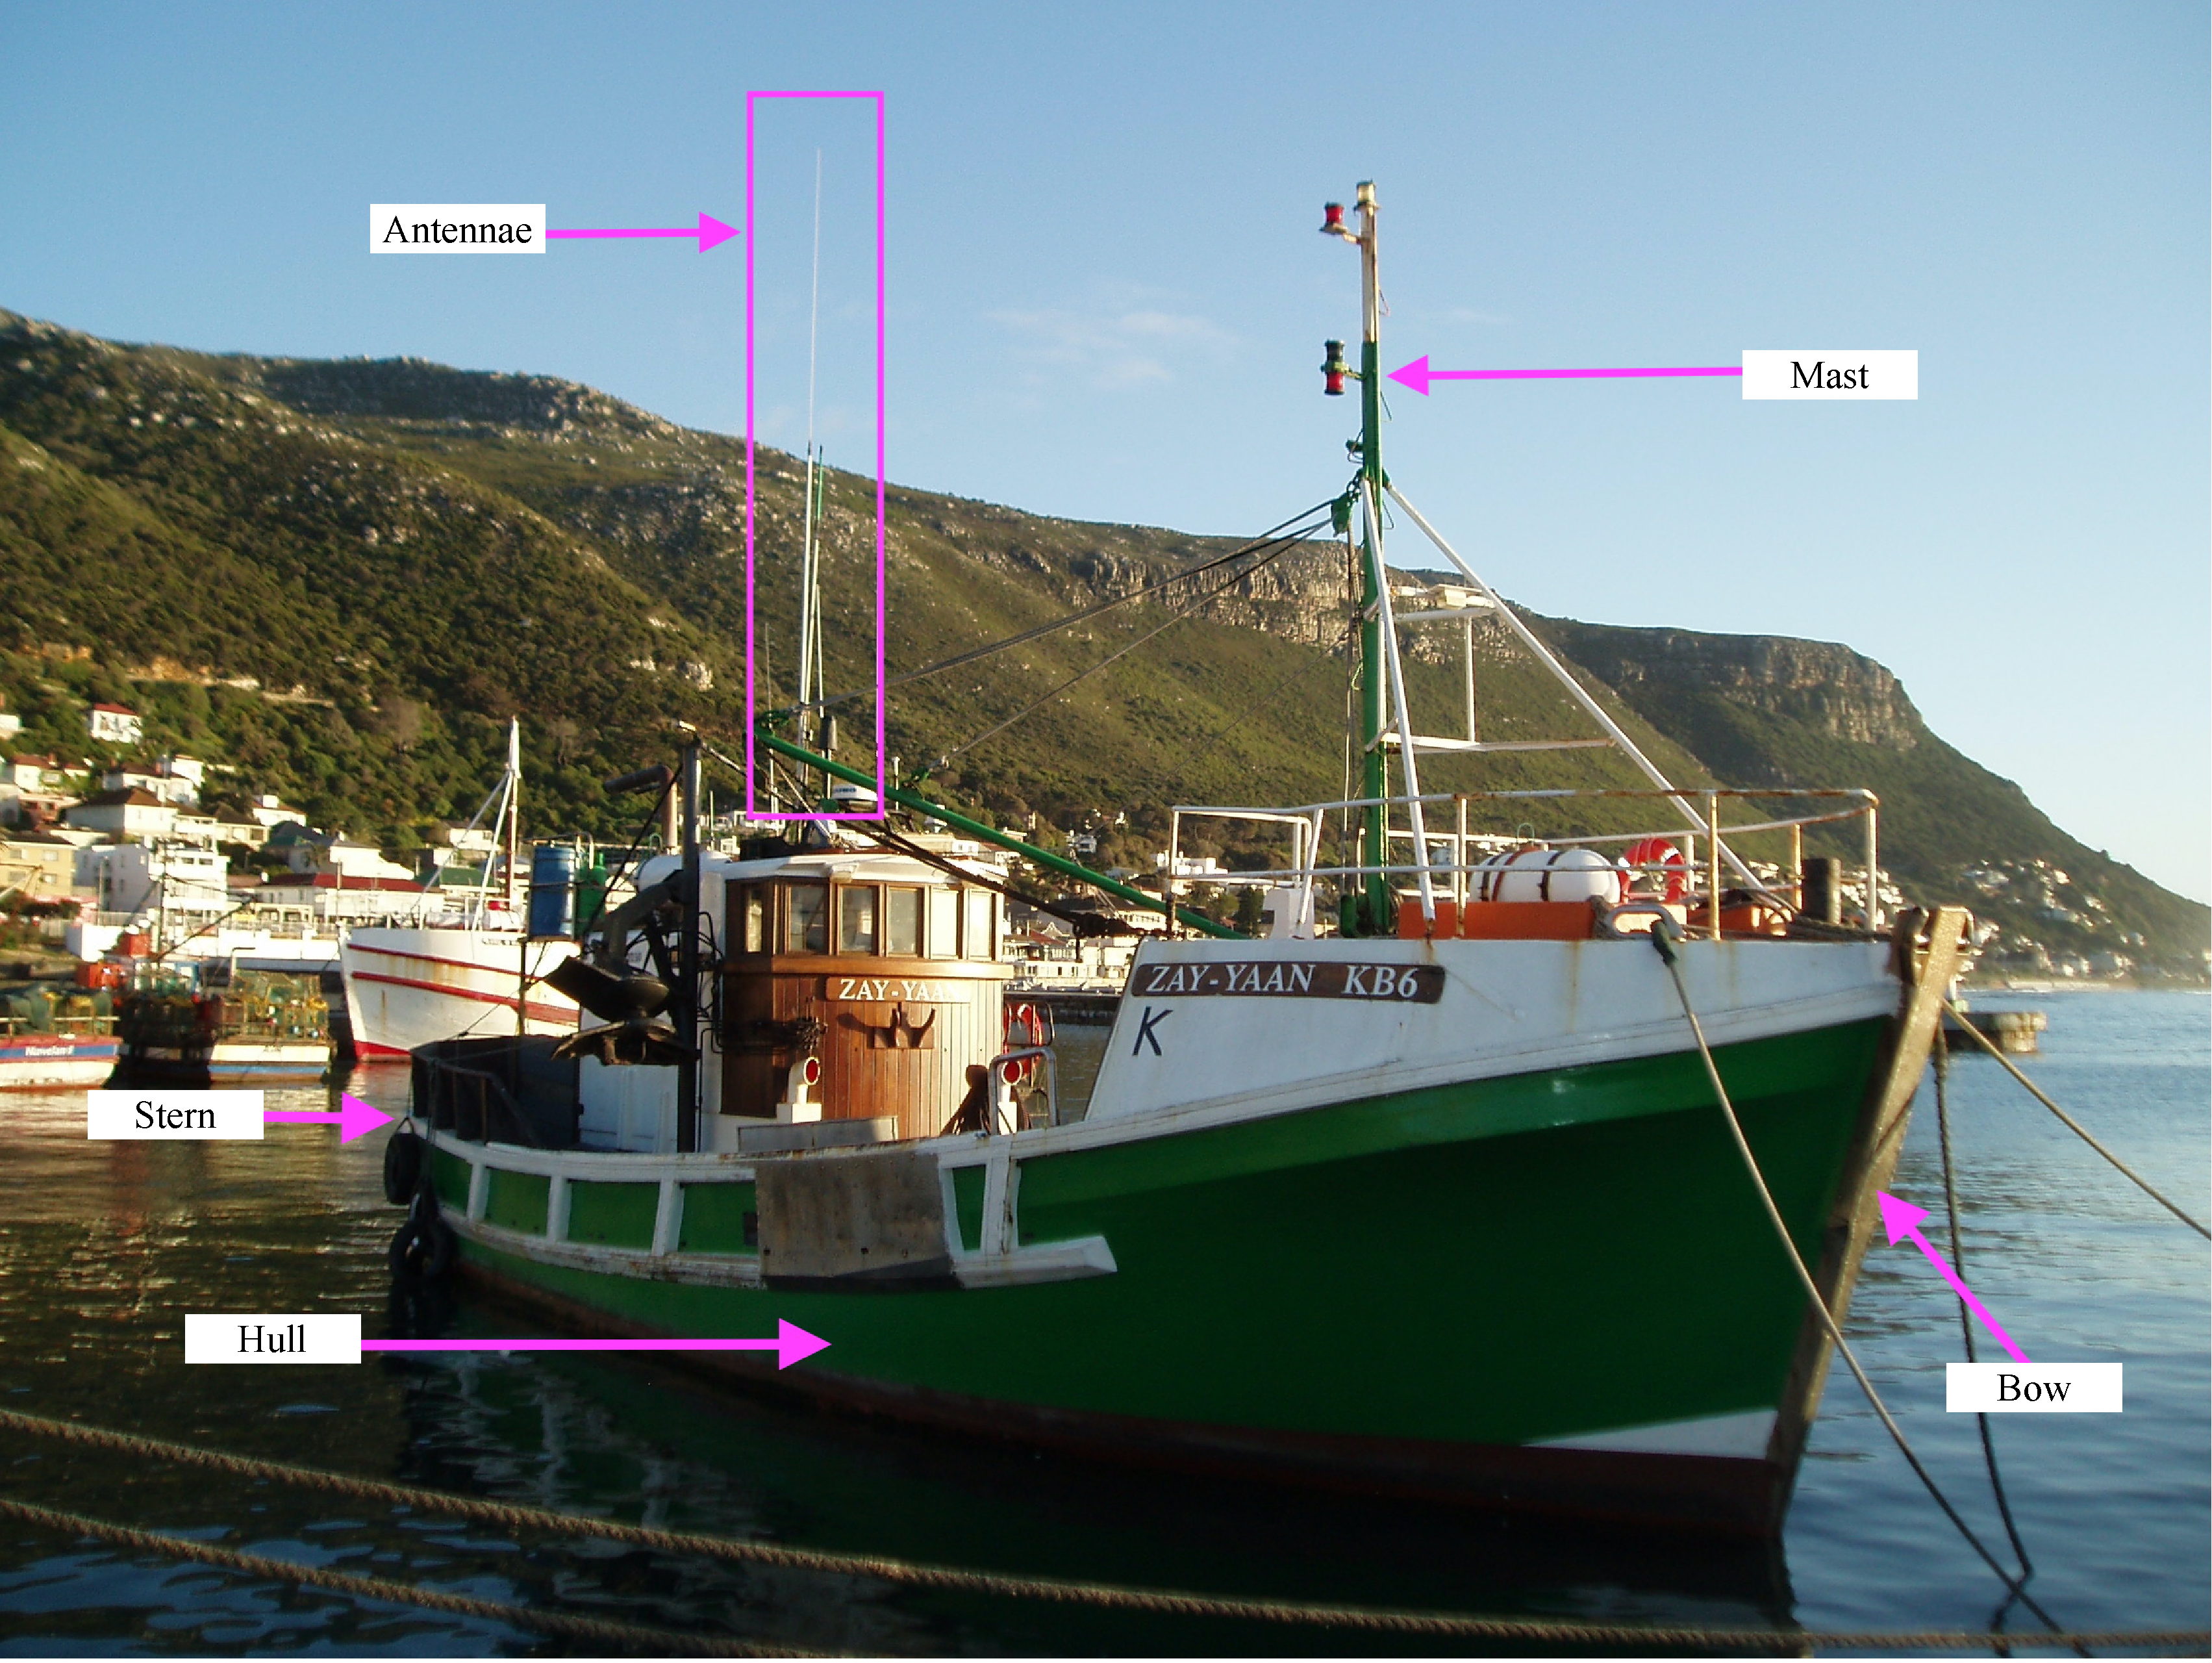
\includegraphics{Figures/04AlgoV&V/Measured/zayyaan.pdf}}
        \caption{Zay-Yaan KB6 boat structure. Adapted from \cite{zayyaan_data}.}
        \label{fig:yuanAF_zayyaan}
        \vspace*{-\baselineskip}
    \end{wrapfigure}
    \autoref{subfig:yuanAF_measured_original} shows the unfocused \gls{isar} image. Comparing it to the image of the \autoref{fig:yuanAF_zayyaan}, the mast and antennae features were poorly represented in the \gls{isar} image. Applying \gls{ra}, resulted in the \gls{isar} image in \autoref{subfig:yuanAF_corrRA_measured_RA} which more accurately represents the boat's features; a thin long rectangular cluster of scatterers clearly shows the antennae and the angular bow of the boat is well reflected. However, this image still exhibited Doppler spreading and sidelobes which could be improved by \gls{af}.

    \autoref{subfig:yuanAF_corrRA_measured_AF} exhibits reduced sidelobes which was attributed to the phase correction performed during \gls{mdsaf}. Additionally, the rectangular group of antennae and triangular shape of the mast represent the features in \autoref{fig:yuanAF_zayyaan}. Thus the image was visually more focused after \gls{mdsaf}.
    
    \begin{figure}[H]
        \centering
        \begin{subfigure}{0.3\linewidth}
            \resizebox{\linewidth}{!}{% This file was created by matlab2tikz.
%
%The latest updates can be retrieved from
%  http://www.mathworks.com/matlabcentral/fileexchange/22022-matlab2tikz-matlab2tikz
%where you can also make suggestions and rate matlab2tikz.
%
\begin{tikzpicture}
\begin{axis}[%
width=5.554in,
height=4.754in,
at={(0.932in,0.642in)},
scale only axis,
point meta min=-40,
point meta max=0,
axis on top,
xmin=0,
xmax=29.6578125,
xlabel style={font=\fontsize{25}{14}\selectfont\color{black}, yshift=-10pt},
xlabel={Range (m)},
ymin=-88.0034,
ymax=86.6175,
ylabel style={font=\fontsize{25}{14}\selectfont\color{black}},
ylabel={Doppler frquency (Hz)},
axis background/.style={fill=white},
tick label style={font=\fontsize{20}{11}\selectfont\color{black}},
xtick distance= 4,             % Set the spacing between x-axis ticks
ytick distance = 10,
colormap/jet,
colorbar
]
\addplot [forget plot] graphics [xmin=0, xmax=29.6578125, ymin=-88.0034, ymax=86.6175] {Figures/04AlgoV&V/Measured/01Original/Measured_ISAR_frame2464.png};
\end{axis}

\end{tikzpicture}%}
            \caption{Unfocused image. \label{subfig:yuanAF_measured_original}}
        \end{subfigure}
        \hspace{0.5cm}
        \begin{subfigure}{0.3\linewidth}
            \resizebox{\linewidth}{!}{% This file was created by matlab2tikz.
%
%The latest updates can be retrieved from
%  http://www.mathworks.com/matlabcentral/fileexchange/22022-matlab2tikz-matlab2tikz
%where you can also make suggestions and rate matlab2tikz.
%
\begin{tikzpicture}
\begin{axis}[%
width=5.554in,
height=4.754in,
at={(0.932in,0.642in)},
scale only axis,
point meta min=-40,
point meta max=0,
axis on top,
xmin=0,
xmax=29.6578125,
xlabel style={font=\fontsize{25}{14}\selectfont\color{black}, yshift=-10pt},
xlabel={Range (m)},
ymin=-88.0034,
ymax=86.6175,
ylabel style={font=\fontsize{25}{14}\selectfont\color{black}},
ylabel={Doppler frquency (Hz)},
axis background/.style={fill=white},
tick label style={font=\fontsize{20}{11}\selectfont\color{black}},
xtick distance= 4,             % Set the spacing between x-axis ticks
ytick distance = 10,
colormap/jet,
colorbar
]
\addplot [forget plot] graphics [xmin=0, xmax=29.6578125, ymin=-88.0034, ymax=86.6175] {Figures/04AlgoV&V/Measured/02CorrRA/SCRA_Measured_ISAR_frame2464.png};
\end{axis}

\end{tikzpicture}%}
            \caption{Range-aligned image. \label{subfig:yuanAF_corrRA_measured_RA}}
        \end{subfigure}
        \hspace{0.5cm}
        \begin{subfigure}{0.3\linewidth}
            \resizebox{\linewidth}{!}{% This file was created by matlab2tikz.
%
%The latest updates can be retrieved from
%  http://www.mathworks.com/matlabcentral/fileexchange/22022-matlab2tikz-matlab2tikz
%where you can also make suggestions and rate matlab2tikz.
%
\begin{tikzpicture}
\begin{axis}[%
width=5.554in,
height=4.754in,
at={(0.932in,0.642in)},
scale only axis,
point meta min=-40,
point meta max=0,
axis on top,
xmin=0,
xmax=29.6578125,
xlabel style={font=\fontsize{25}{14}\selectfont\color{black}, yshift=-10pt},
xlabel={Range (m)},
ymin=-88.0034,
ymax=86.6175,
ylabel style={font=\fontsize{25}{14}\selectfont\color{black}},
ylabel={Doppler frquency (Hz)},
axis background/.style={fill=white},
tick label style={font=\fontsize{20}{11}\selectfont\color{black}},
xtick distance= 4,             % Set the spacing between x-axis ticks
ytick distance = 10,
colormap/jet,
colorbar
]
\addplot [forget plot] graphics [xmin=0, xmax=29.6578125, ymin=-88.0034, ymax=86.6175] {Figures/04AlgoV&V/Measured/05YuanAF/YuanAF_SCRA_Measured_ISAR.png};
\end{axis}

\end{tikzpicture}%}
            \caption{Autofocused image.\label{subfig:yuanAF_corrRA_measured_AF}}
        \end{subfigure}
        \caption{\gls{isar} images formed using the original, Correlation range-aligned and \gls{mdsaf} autofocused \gls{hrr} profiles of a single measured data frame.} \label{subfig:yuanAF_corrRA_measured}
    \end{figure}

    Additionally, the \gls{ic} values were used to quantitively examine the improvement of image focus. The \gls{ic} values were \textbf{7.0534}, \textbf{8.1803} and \textbf{17.0869} for the images in \autoref{subfig:yuanAF_corrRA_measured}(a),(b) and (c), respectively. The \gls{ic} improvement factor after \gls{ra} and \gls{af} was calculated to be \(\frac{17.0869-8.1803}{8.1803}=108.88\%\) which further indicated that the \gls{mdsaf} improved the focus of the \gls{isar} image.

    Importantly, the focused image in \autoref{subfig:yuanAF_corrRA_measured_AF} still exhibited Doppler spreading which was attributed to sidelobes in the measured data, as discussed in \autoref{theory:sidelobes}. However, the image displayed a good characterisation of the boat's features despite the Doppler spreading.

    Therefore, the improved implementation of the \gls{mdsaf} algorithm produced a more focused image of measured data and was validated for use in this report.
    
%%%%%%%%%%%%%%%%%%%%%%%%%%%%%%%%%%%%%%%%%%%%%%%%%%%%%%%%%%%%%%%%%%%%%%%%%%%%%%%%%%%%%%%%%%%%%%%%%%%%
\section{Optimisation of Implementation to Reduce Runtime \label{sec:V&V_optimisation}}
The algorithms implemented in this chapter are designed for use in a \gls{qlp}. To decrease the runtime of the processor, the algorithm implementations were optimized.

\textsc{MATLAB} is designed to operate on arrays and matrices and has built-in functions that enable multithreaded processing of matrix operations. This eliminates the need for iterative loops required in other programming languages. The implementation of all algorithms used in this report leveraged these capabilities to achieve improved runtime performance.  Additionally, find() was replaced with \textsc{MATLAB} logical indexing \cite{MATLAB_logical_indexing} where possible. All optimisation changes and adjustments were carefully checked to ensure that the same results were produced. 

    %***************************************************************************************%
    \subsection{Correlation Range Alignment Algorithm}
    Cross-correlation can be performed in the time or frequency domain, \cite{ISARtextbook_Martorella} states that the frequency domain computation is faster. However, \textsc{MATLAB} has a built-in two-dimensional time domain cross-correlation function that is optimised for \textsc{MATLAB} use. This made the time domain calculation faster than performing multiple steps to do the frequency domain correlation in this \textsc{MATLAB} specific implementation. Notably, the final script achieved a x reduction in runtime compared to the initial version.
    
    %***************************************************************************************%
    \subsection{Haywood Range Alignment Algorithm}
    The initial implementation was revised for further optimisation. This process involved introducing global parameters to reduce the frequency of function calls.  In the initial version, the correlation \gls{ra} algorithm was used to perform cross-correlation, while in the revised script, this operation was directly integrated into the code. This revision not only reduced runtime but also removed the dependence on another algorithm. Notably, the final script achieved a x reduction in runtime compared to the initial version.
    
    %***************************************************************************************%
    \subsection{Haywood Autofocus Algorithm}
    Further optimisation was achieved by introducing global parameters to reduce the frequency of function calls. While this adjustment required the code to be restructured, it still yielded the same results. Notably, the final script achieved a x reduction in runtime compared to the initial version.

    %***************************************************************************************%
    \subsection{Yuan Autofocus Algorithm}
    The \textsc{MATLAB} functions used to calculate values in the algorithm were optimized to use faster alternatives that still yielded the correct results. For example, the mink() function, which returns the index of the smallest k values, was replaced by the the sort() function, and the returned array was then indexed. This change was made because sort() is multithreaded, and resulted in runtime improvements. Notably, the final script achieved a x reduction in runtime compared to the initial version.
    %***************************************************************************************
    \subsection{Runtime Testing}
    To ensure that the changes made to each algorithm resulted in runtime improvements, the algorithms before and after optimisation were timed.
    \subsubsection{Testing Setup}
    A \textsc{MATLAB} \href{}{timing script} was used to measure the runtime of each algorithm, before and after optimisation. This script was used to execute each algorithm 100 times and the raw timing results were recorded in a CSV file. The timing tests were performed on a single simulated \gls{isar} frame,  which had 32 profiles, each with 256 range bins. A folder containing the testing files is available on \href{}{GitHub}.

    The testing was conducted on a MacBook Pro (2016) with the following hardware specifications:
    \begin{itemize}
        \item Processor: 2.9GHz Dual-Core Intel Core i5
        \item Memory: 8GB 2133MHz LPDDR3
    \end{itemize}

    \subsubsection{Results}
    The raw timing results recorded in the \href{}{CSV file} were averaged to determine the effective runtime of each algorithm. \autoref{tab:optimisation_timing} contains the effective runtime of each algorithm before and after runtime optimisation. The runtime improvement was calculated as
    \begin{equation}
        Improvement = \frac{Original-Optimised}{Original}
    \end{equation}
    and is recorded in \autoref{tab:optimisation_timing}.

    \begin{table}
        \centering
        \begin{tabular}{|l|c|c|c|}
            \hline
            \multicolumn{1}{|c|}{\textbf{Algorithm}} & \textbf{Original Runtime (s)}&\textbf{Optimised Runtime (s)} &\textbf{Improvement (\%)} \\
            \hline
            Correlation \gls{ra}    & 0.009556872 & 0.002843406 & 70.24 \\
            \hline
            Haywood \gls{ra}        & 0.011963056 & 0.004136744 & 65.42  \\
            \hline
            \gls{sdsaf}             & 0.002407375 & 0.001363729 & 43.35  \\
            \hline
            \gls{mdsaf}             & 0.002260847 & 0.001801478 & 20.31 \\
            \hline
        \end{tabular}
        \caption{Algorithm runtime optimisation timing results. \label{tab:optimisation_timing}}
    \end{table}

    The results recorded in \ref{tab:optimisation_timing} show that for all algorithms the optimisation strategies resulted in improved runtimes.

%%%%%%%%%%%%%%%%%%%%%%%%%%%%%%%%%%%%%%%%%%%%%%%%%%%%%%%%%%%%%%%%%%%%%%%%%%%%%%%%%%%%%%%%%%%%%%%%%%%%
\section{Summary}
\begin{itemize}
    \item The integer bin shifting limitation of the Correlation \gls{ra} algorithm prevented perfect alignment of the \gls{hrr} profiles in both simulated and measured data.
    \item The Haywood \gls{ra} realised fractional bin shifts and produced range-aligned profiles in both simulated and measured data.
    \item In measured data, there was often more than one \gls{ds}. A limitation of the \gls{sdsaf} was that it used only one \gls{ds} to focus the \gls{isar} image. This limited how well the image could be focused when using measured data. A \gls{sf} was introduced to ensure a high-power \gls{ds} was selected. This subsequently improved the performance of the algorithm. \gls{sdsaf} produced satisfactorily focused images for measured data.
    \item \gls{mdsaf} realised the use of multiple \gls{ds}s to focus the image. The algorithm's performance was improved by adding noise filtering and a systematic way of selecting the reference profile. \gls{mdsaf} produced focused images for measured data.
    \item The processing time of all algorithms was successfully reduced through optimisation of the implementations.
\end{itemize}
% ----------------------------------------------------
\ifstandalone
\bibliography{../Bibliography/References.bib}
\printnoidxglossary[type=\acronymtype,nonumberlist]
\fi
\end{document}
% ----------------------------------------------------